%% 
%% Copyright 2007-2024 Elsevier Ltd
%% 
%% This file is part of the 'Elsarticle Bundle'.
%% ---------------------------------------------
%% 
%% It may be distributed under the conditions of the LaTeX Project Public
%% License, either version 1.3 of this license or (at your option) any
%% later version.  The latest version of this license is in
%%    http://www.latex-project.org/lppl.txt
%% and version 1.3 or later is part of all distributions of LaTeX
%% version 1999/12/01 or later.
%% 
%% The list of all files belonging to the 'Elsarticle Bundle' is
%% given in the file `manifest.txt'.
%% 
%% Template article for Elsevier's document class `elsarticle'
%% with numbered style bibliographic references
%% SP 2008/03/01
%% $Id: elsarticle-template-num.tex 249 2024-04-06 10:51:24Z rishi $
%%
\documentclass[preprint,review,11pt, authoryear]{elsarticle}
\usepackage[margin=1.2in]{geometry}  % 1-inch margins on all sides
\usepackage{lineno}
\usepackage{csquotes}\usepackage{url}
\usepackage[hyphens]{url}
\usepackage{xurl}   % better URL line breaking
\usepackage{multirow}
\usepackage[final]{changes}
\setlength{\parindent}{0pt}
\usepackage{booktabs}
\usepackage{longtable}
\usepackage{float}
\usepackage{booktabs}
\usepackage{soul,color}
\usepackage{empheq}
\usepackage{graphicx}
\usepackage{eurosym}
\usepackage[colorinlistoftodos]{todonotes}
\usepackage{longtable}
\usepackage{hyperref}
\usepackage{subcaption}
\usepackage{xcolor}
\usepackage{enumitem}
\usepackage{amssymb}  % For \checkmark
\usepackage{mdframed}
%\usepackage[printonlyused ]{acronym}
\usepackage{acronym}
\usepackage{xcolor} % For colored text
\usepackage{marginnote} % For margin notes
\definecolor{customblue}{HTML}{003049} % Replace with your preferred hex code
\newcommand{\newcontent}[2]{%
  \textcolor{customblue}{#1}% Highlight new content in blue
  \marginnote{\tiny\raggedright Edited: #2}% Add a margin note with the edit date
}
%% Use the option review to obtain double line spacing
%% \documentclass[authoryear,preprint,review,12pt]{elsarticle}
\usepackage{titlesec}

% Redefine \paragraph to look like a subsection
\titleformat{\paragraph}[block]   % block = line break, not run-in
  {\normalfont\normalsize\itshape} % font
  
  {\theparagraph} % label
  {1em}          % spacing between label and title text
  {}             % before-code
\titlespacing*{\paragraph}
  {0pt}{1ex plus .2ex}{0.3ex} % {left}{before}{after}

% Optional: remove numbering if you don't want it
\setcounter{secnumdepth}{4}  % keep numbered
% \setcounter{secnumdepth}{3}  % unnumber paragraph headings

\newcommand{\cmark}{\ding{51}}  % Checkmark
%% Use the options 1p,twocolumn; 3p; 3p,twocolumn; 5p; or 5p,twocolumn
%% for a journal layout:
%% \documentclass[final,1p,times]{elsarticle}
%% \documentclass[final,1p,times,twocolumn]{elsarticle}
%% \documentclass[final,3p,times]{elsarticle}
%% \documentclass[final,3p,times,twocolumn]{elsarticle}
%% \documentclass[final,5p,times]{elsarticle}
%% \documentclass[final,5p,times,twocolumn]{elsarticle}

%% For including figures, graphicx.sty has been loaded in
%% elsarticle.cls. If you prefer to use the old commands
%% please give \usepackage{epsfig}

%% The amssymb package provides various useful mathematical symbols
\usepackage{amssymb}
%% The amsmath package provides various useful equation environments.
\usepackage{amsmath}
%% The amsthm package provides extended theorem environments
%% \usepackage{amsthm}

%% The lineno packages adds line numbers. Start line numbering with
%% \begin{linenumbers}, end it with \end{linenumbers}. Or switch it on
%% for the whole article with \linenumbers.
%% \usepackage{lineno}

\journal{Transportation Research Part D: Transport and Environment}

\begin{document}
% without table print
\acrodef{CCGT}[CCGT]{Combined-cycle gas turbines}
\acrodef{CD}[CD]{charging demand}
\acrodef{CT}[CT]{charging types}
\acrodef{CP}[CP]{charging processes}
\acrodef{DC}[DC]{direct current}
\acrodef{DA}[DA]{day-ahead}
\acrodef{DSM}[DSM]{demand-side management}
\acrodef{EV}[EV]{electric vehicle}
\acrodef{ENTSOE}[ENTSO-E]{European network of transmission system operators}
\acrodef{FBMC}[FBMC]{flow based market coupling}
\acrodef{LP}[LP]{linear programming}
\acrodef{MBCM}[MBCM]{market-based congestion management}
\acrodef{MILP}[MILP]{mixed integer linear programming}
\acrodef{NT}[NT]{National Trends}
\acrodef{NECP}[NECP]{national energy and climate plans}
\acrodef{NSE}[NSE]{not supplied energy}
\acrodef{NTC}[NTC]{net transfer capacities}
\acrodef{OM}[O\&M]{operation and maintenance costs}
\acrodef{PHS}[PHS]{pumped hydro-power storage units}
\acrodef{PTDF}[PTDF]{power transfer distribution factor}
\acrodef{PV}[PV]{photovoltaic}
\acrodef{RESE}[RES-E]{renewable energy sources for electricity}
\acrodef{RoR}[RoR]{run-of-the-river hydroelectricity}
\acrodef{SEW}[SEW]{Socio-economic welfare}
\acrodef{SRMC}[SRMC]{short run marginal costs}
\acrodef{TSO}[TSO]{transmission system operator}
\acrodef{V2G}[V2G]{vehicle-to-grid}
\acrodef{VoLL}[VoLL]{value of lost load}
\acrodef{TSO}[TSO]{transmisison grid operator}
\acrodef{HDT}[HDT]{heavy-duty truck}
\acrodef{LDT}[LDT]{light-duty truck}

\begin{frontmatter}

%% Title, authors and addresses

%% use the tnoteref command within \title for footnotes;
%% use the tnotetext command for theassociated footnote;
%% use the fnref command within \author or \affiliation for footnotes;
%% use the fntext command for theassociated footnote;
%% use the corref command within \author for corresponding author footnotes;
%% use the cortext command for theassociated footnote;
%% use the ead command for the email address,
%% and the form \ead[url] for the home page:
%% \title{Spatial granularity matters: participation ofcommercial electric fleets for redispatch in congested transmission grids\tnoteref{label1}}
%% \tnotetext[label1]{}
%% \author{Name\corref{cor1}\fnref{label2}}
%% \ead{email address}
%% \ead[url]{home page}
%% \fntext[label2]{}
%% \cortext[cor1]{}
%% \affiliation{organization={},
%%             addressline={},
%%             city={},
%%             postcode={},
%%             state={},
%%             country={}}
%% \fntext[label3]{}

% \title{Dynamics in the vehicle turnover of passenger cars --- insights to the regional implementation of global energy system decarbonization pathways}
% \title{The importance of density and expansion speed in the rollout of public charging infrastructure and its potential to accelerate the electrification of the passenger car vehicle stock}
\title{Public Charger Expansion: Impacts Across Income Classes and Beyond Regional Borders}
%% use optional labels to link authors explicitly to addresses:
\author[label1]{Antonia Golab\footnote{Corresponding author. E-mail: golab@eeg.tuwien.ac.at}}
\author[label1,label2]{Sebastian Zwickl-Bernhard}
\author[label1,label2]{Hans Auer}

\affiliation[label1]{organization={Energy Economy Group (EEG), Technische Universität Wien},
            addressline={Gusshausstraße 25-29, E370-3},
            city={Vienna},
            postcode={1040},
            country={Austria}}

\affiliation[label2]{organization={Department of Industrial Economics and Technology Management, The Norwegian University of Science and Technology},
            addressline={Alfred Getz vei 3},
            city={Trondheim},
            postcode={7491},
            country={Norway}}

% \author{Antonia Golab} %% Author name

% %% Author affiliation
% \affiliation{organization={},%Department and Organization
%             addressline={}, 
%             city={},
%             postcode={}, 
%             state={},
%             country={}}

%% Abstract

%% Text of abstract
\begin{abstract}

Public charging infrastructure is crucial to meet the charging needs of diverse consumer groups, and anticipating future patterns is essential for electricity system planning. This study examines optimal infrastructure roll-out from two perspectives: (1) how spatial densification strategies influence consumer groups with varying adoption behaviors, and (2) how local charging expansion affects battery-electric vehicle (BEV) adoption in neighboring regions. A techno-economic optimization framework is applied, incorporating intangible costs from charging time across charger types. The method integrates long-term infrastructure planning, BEV adoption by consumer group, allocation of charging processes, and spatial interactions between regions. Using a case study of the Basque Country, results show that charger network density significantly shapes charging behavior across income classes. Additionally, rapid local expansion \added{(+30\% to a baseline expansion)} has a positive, though modest, spillover effect on BEV adoption in adjacent regions \added{(max. 2.1\%)}.
\end{abstract}

%%Graphical abstract
%\begin{graphicalabstract}
%
\includegraphics{grabs}
% \end{graphicalabstract}

%%Research highlights


\begin{highlights}
    \item Fueling detouring time results in improved service from network densification.
    \item Techno-economic optimization shows \added{moderate} spillovers of local roll-out on regional BEV adoption.
    \item Income-based consumer classes are key for planning charging networks by usage patterns.
\end{highlights}

%% Keywords
\begin{keyword}
       passenger BEV adoption, income classes, charger station distribution, charging infrastructure expansion, spillover effect, infrastructure expansion speed
\end{keyword}
% \hl{TODOs:}
% \begin{itemize}
%     \item highlights new
%     \item RQs nachschärfen / vor allem NUTS-2 regions vs NUTS-3 
%     \item qfuelinfr in methodenbeschreibung mit textrm nachkorrigieren
%     \item title 4.2 is wierd
%     \item results: make y title (electrification share) all same
%     \item figure 12: double info on scenario
%     \item think about extending also commuting charging behavior of origin bizkaia and betwen araba and gipuzkoa
%     \item appendix: validation vehicle stock sizing
% \end{itemize}
\end{frontmatter}

%% Add \usepackage{lineno} before \begin{document} and uncomment 
%% following line to enable line numbers
%% \linenumbers

%% main text
%%

%% Use \section commands to start a section
%\linenumbers  % Start line numbering
% \begin{acronym}
%     \acro{BEV}{battery-electric vehicle}
%     \acro{VoT}{value of time}
%     \acro{LoS}{Level of Service}
%     \acro{MILP}{Mixed-integer linear program}
% \end{acronym}
\section{Introduction} 

    With the decarbonisation targets set for the different sectors of the energy system approaching, the efficient allocation of investments to integrate low-carbon technologies becomes increasingly urgent. One important lever is the build-up of related infrastructures that enable the sustainable deployment of these technologies \citep{KLITKOU201522}. In the transport sector, these infrastructures include the public charging infrastructure supporting the deployment of battery-electric vehicles (BEVs) in \deleted{the} road transport \citep{STAJIC2023100658}. While in many European Union (EU) countries, the \replaced{build-up}{built-up} of the infrastructure is in-line with EU goals \citep{transport2024afir}, recent adoption numbers of BEVs in the passenger car sector (f.e. 15.4\% market share in May 2025 in EU countries \citep{acea2025may}) indicate that the BEV passenger car fleet is not growing in line with the EU's objective of 100\% market share of zero-emission vehicles in 2035 \citep{tmleuven2025zeroemission}. 

    The expansion of the public charging infrastructure has been a central part of the ``Sustainable \& Smart Mobility Strategy'' paper by the European Commission \deleted{(EU)} \citep{eu2021mobility}. The goal of the expansion plans is defined at \added{the} EU country level \citep{transport2024afir}, while the regional and local policies direct the demand-targeting allocation \citep{LAMONACA2022111733}. Scientific literature on charging infrastructure planning has focused largely on allocating public charging infrastructure to set up an initial network and meet the charging demand of early adopters \citep{METAIS2022111719, https://doi.org/10.1002/wene.306}. These early adopters are characterized as being of high-income classes and homeowners \citep{BRUCKMANN2021102615}. Currently, the significant majority of charging processes take place at home \citep{BARESCH2019388} and empirical case studies have found that there is a disparity in the availability for potential adopters of different income classes \citep{GAZMEH2024104222}. While in the long-term perspective, BEVs need to be adopted by passenger car owners of all socio-economic backgrounds \citep{HOPKINS2023113398}, this will also shift the current central role of home chargers to public chargers.
    
    This shift is accompanied by an increasingly better range, and therefore reduced range anxiety, allowing for higher flexibility in allocating individual charging demand \citep{SPAVEN2022133349}. Empirical studies have already shown that the local deployment of public charging infrastructure does not only impact BEV adoption rates within a region but the adoption rate in neighboring regions \citep{QIAN2024104400}. This has been observed on the country or state level and the neighborhood level \citep{SELENASHENG2022103256}. These cross-border interactions add an extra layer of complexity to the long-term charger roll-out.

    The aim of this paper is to gain \added{a} better understanding in the two following aspects: the impact of public charging infrastructure roll-out on the BEV adoption in different income classes, and, the cross-border (i.e., spill\deleted{-}over \footnote{\added{We use this term based on the assumption that the charging infrastructure is locally installed exclusively with the aim to serve exclusively the local charging demand.}}) of \deleted{a} local deployment strategy. Here\deleted{by}, two determining factors of\deleted{the } infrastructure roll-out are focused on: the spatial density and the speed of the deployment. 
    % These aspects are analysed on the scale of federal states (NUTS-2)\footnote{A detailed description of the NUTS nomenclature can be found in \citep{eurostat_nuts}} and provinces (NUTS-3). 
    Consequently, the research questions are as follows: 
    
    \begin{mdframed}
        \begin{itemize}
            \item[\textbf{RQ1:}] To what extent does the spatial \replaced{density}{distribution} of public charging infrastructure influence battery-electric vehicle adoption across consumers with different income levels?

            \item[\textbf{RQ2:}] How does a local rapid charging infrastructure expansion affect the adoption of battery-electric vehicles in neighboring regions with slower charging infrastructure expansion? 
        \end{itemize}
    \end{mdframed}
    
    These research questions together address the BEV adoption of two types of consumers: consumers of different income\deleted{-class} levels and consumers in neighboring regions. These questions are methodologically addressed from a system-cost-\replaced{optimization perspective}{optimal view} of the decarbonization of the passenger car fleet. We build on previous work that has used the measure of time to model the BEV adoption for consumers of different income levels \citep{TATTINI2018265} and connect this with work that considers \deleted{the }time consumption dependent on different charging patterns \citep{luh2022behavior}. We introduce the detouring time as an endogenous decision variable. This allows us to link the expansion of public charging infrastructure to the increase in spatial density of the charger network, and, therefore, to \deleted{the }decreased consumers' total travel time. To capture cross-regional interactions, we focus our analysis \replaced{at}{on} \replaced{the regional level (NUTS-2)}{the spatial scale of a European federal state} and use traffic flow and socio-economic data of the Basque Country, Spain. 
    
    % These research questions tackle the large-scale adoption by means of diverse consumer groups in two directions, i.e. first, the interaction between local charging infrastructure expansion and the BEV adoption of consumers of different income levels; second, the interaction BEV adoption of consumers in neighboring regions. 
    
    
    % \citet{luh2022behavior} and \citet{TATTINI2018265}. \citet{luh2022behavior} have considered the adoption of BEVs based on travel and charging times for different charging types, while \citet{TATTINI2018265} have considered the measure of time to 

    
    
    
    
    % The methodology of this paper is based on the formulation of a system-cost-minimizing mixed-integer-linear program (MILP) that models the technology change within the vehicle stock, charging infrastructure investments, and the allocation of charging activity between different charging opportunities. The core functionalities comprise the consideration of different consumer groups that vary by income level and the endogenous modeling of increased density of charging stations through the expansion of the public charging infrastructure network. Based on this, the impact of different deployment strategies is analysed, in particular the impact on the vehicle stock turnover towards a battery-electric vehicle stock fleet.
    
    % Already empirical research has found spillover effect ... of pubkic charging infrastrucur e on neighbouring 
    
    
    % It has been evident that local charging infrastructure not only has a positive impact on the BEV adoption in the 
    
    % A passenger BEV currently remains to be a luxory item that are mostly owned by households of high-income classes with home ownership \citet{BRUCKMANN2021102615}. The main barriers for the adoption include the high costs for the purchase of a BEV and a limited availibility of charging infrastructure \citet{STAJIC2023100658}. These two barriers have been addressed by a wide range of policies, f.e., by the subsidization, tax benefits and non-monetary benefits \citet{ANILAN2024104424}. Currently, most charging activity takes place at home chargers \citet{BARESCH2019388}. With the shift from early adopters to the large-scale adoption of BEVs, It is to be expected that the role of public charging infrastructure will gain significantly in importance \citep{engel2018charging}. 
    
    % On the geographically lower level, the exact placement of public charging stations is planed in alignment with the charging demand of early adopters and with the goal of enhancing the convenience for the charging process and decreasing range anxiety  \citep{Asensio2021}. This goes along with understanding the mobility patterns of BEV drivers and their charging behavior \citep{VISARIA2022120}. As the large-scale adoption is still ahead, the future re-charging behavior of is still unknown, which gives also potential to still shaping charging behavior, for example, by allocating charging infrastructure conveniently for potential BEV drivers, at origins or destinations points or en-route, while being able to also consider system optimality in regard to minimize the costs for the expansion of charging infrastructure \citep{METAIS2022111719}. This describes the functionality in most of proposed charging infrastructure planning tools that specifically plan charging infrastructure for early BEV adopters \citet{https://doi.org/10.1002/wene.306}. A diverse consumer group with varying income-levels, which goes along with large-scale BEV adoption, is rarely addressed in this context.
    
    % Another neglected aspect in region-level charging infrastructure planning is the consideration of cross-boarder effects.
    
    
    % where should we be? where are we? why are we there? (BEV still as luxory item, less increase as expected; multiple car brands not wanting to achieve the goals; slowing down rates; postponing of decarbonization goals) Main barriers for this are the still the high costs of technology + charging technology (speed) + infrastructure availibility.
    % What schemes are there for making evs affordable -> subsidization \dots. Current owners are rich and homeowners, with charging happening at home [REF]. this is changed and shifted with increase of BEV adoption. importance of public charging infrastructure grows 
    
    % On EU level, goal of continuously enhancing the public charging infrastructure availbility. translated to country level: policy making, f.e. subsidization/ausschreibungen \textit{find REF here} \dots Charging infrastructure is allocated to meet demand and enhance convenience of owning a BEV in terms of providing placing the charging infrastructure at POIs and providing a dense network [REF]. Goes along with understanding mobility patterns of BEV users and charging behavior. On the one hand, this is going to change and it still to be shaped by the deployment of charging infrastructure \dots 

    % Studies have shown spillover effect of local charging infrastructure, effecting bev adoption in neighbouring regions on \dots level (which geographic level?) which has not yet been addressed explicitly in the context of long-term public charging infrastructure planning.

    


    \newpage
% \section{Introduction} \label{ref:intro}

%     \hl{\textbf{TODO: the problem statement needs to be here more accurate/ WHAT IS THE PROBLEM STATEMENT??}}
%     \paragraph{Acceleration of the BEV fleet required}
%     where should we be? where are we? why are we there? (BEV still as luxory item, less increase as expected; multiple car brands not wanting to achieve the goals; slowing down rates; postponing of decarbonization goals)

%     \paragraph{The importance of time in transport}
%     time in service; people have been increasingly increasing the amount of travel distance by using transport services with more speed; convienence and time very relevant in the choice of travel mode; BEV in this regard: downside charging; a way to reduce it; large literature dedicated to allocation charging infrastructure in such a way that it is most convinient to charge; in comparison to conventional fossil fuel stations - these are allocated more to the needs of first adopters; 

%     also nb one: home charging; but in the long-term not possible in such a way when non-homeowners adopt vehicles; expansion and densification / charging infrastructure availability very relevant factor; reducing distance 
    
%     \paragraph{Regional planning of charging infrastructure}
%     EU goals for country level; rate of public charging infrastructure; \textit{Is it sufficient?}; translating these to the regional level; also interaction and impact between the regions 
    
%     % \citep{HOPKINS2023113398}: analyse in-equity of charging infrastructure roll-out; emphasizing also the lack of second-hand market as well as accessibility of affordable charging infrastructure/ uneven charging infrastructure distribution / availability 

%     \paragraph{Our work given this background}
%      We contribute to the existing literature by bridging the gap between the research on the adoption of battery-electric passenger cars by customers of different income classes and the roll-out strategies of public charging infrastructure. 
%     In the present work, we aim to tackle the question of effective investments in charging infrastructure, focusing on two dimensions: the spatial density of the public charging infrastructure and speed of build-up of public charging infrastructure. This is analyzed at the aggregation level of NUTS-2 regions with the consideration of long-term charging infrastructure investment paths and its impact on the vehicle adoption in different income classes. The research questions addressed here are as follows: 

%     \paragraph{Problem Statement:}
%     overarching: NUTS-2 level region roll-out strategies 
%     \begin{itemize}
%         \item no income classes are addressed 
%         \item the spillover effect is not addressed 
%     \end{itemize}
    
%     \subsection{Research questions}
    
%     \begin{mdframed}
%         \begin{itemize}
%             \item[1] \textit{(preliminary)} 
%             To what extent does the spatial distribution of public charging infrastructure (concentrated vs. distributed) influence battery-electric vehicle adoption across income groups within NUTS-2 regions?
%             %How do spatial density of public charging infrastructure—concentrated versus distributed—affect battery-electric vehicle adoption across income levels for the mobility within NUTS-2 regions?
%             %How do different approaches in charging infrastructure expansion related to the density of charging sites the adoption of battery-electric vehicles in different income classes? 

%             \item[2] \textit{(preliminary)} How does a local rapid charging infrastructure expansion affect the adoption of battery-electric vehicles in neighboring regions with slower charging infrastructure expansion within a NUTS-2 region? 
%         \end{itemize}
%     \end{mdframed}

%     We address these research questions by formulating a system-cost-minimizing mixed-linear-integer program that models the technology change within the vehicle stock, charging infrastructure investments and the allocation of charging activity between different charging opportunties. A core functionality is thereby the consideration of different consumer groups that vary by income level. Based on this, the impact of different strategies for the spatial densification and expansion speed are analysed, in specific their impact on the vehicle stock turnover towards a battery-electric vehicle stock fleet.
    % \begin{itemize}
    %     \item still slow adoption rates/ investment subsidies fall away; 
    %     \item passenger BEV still luxory item 
    %     \item Time is money. already fueling time is issue but then also the detouring
    %     \item Why federal states level? --- find sources!  / goals on country level defined by european commission; incentivization on country level; --- policies on region level ;\citep{JRC101040}; regional implementation of infrastructure projects; we are in the implementation phase for green technologies; investments have to be made; where decision making is happing on regional; 
    %     \item for international level/ highway infrastructure; policies of EU level target; 
    %     \item ein absatz mit wisseschaftlicher abgrenzung; vor allem was die geographische ebene betrifft
    %     %https://www.interregeurope.eu/policy-learning-platform/events/expanding-e-mobility-at-regional-level
    %     %  
    %     \item \textit{Detouring Time:} The extra time needed for reaching to the closest available charging station including the extra driving and walking to your destination
    % \end{itemize}
    %         \citep{TATTINI2018265}: representation of modal choice in energy systems via including VoT; income class based 
    %     \citep{LUO2024104733}: modelling technology adoption first, then long-term expansion planning on grid level; at high resolution / including VoT in objective function
            
    %         \citep{LAMONACA2022111733}: home charging has been convenient option; but will shift towards public charging infrastructure 
    % points to make: value of time is crucial component in the adoption of bev technology
    % \textbf{Problem statement:} Increasing BEV adoption in all income classes with strategic charging infrastructure planning; on a local level; and cross-boarder impacts in the adoption
    %     \citep{martiskainen2021vulnerability}: on energy and transport poverty; clean technologies are expensive 
    % \hl{\textbf{TODO:} \textit{what are nuts regions }}
    
    
    
    
%% Use \subsection commands to start a subsection.

\section{Literature review}

    

    \subsection{Role of income-class level in BEV adoption}

    The level of income has been proven to be a significant predictor for the purchase of a BEV in many studies \citep{AUSTMANN2021101846}. The amount of disposable income influences the frequency of the acquisition of a new passenger car and whether it is purchased on the first or second-hand market \citep{STAJIC2023100658, VALENZUELALEVI2021161}. There exists a wide range of choice models that relate the decision of BEV purchase to socio-economic variables and reveal the influence\deleted{s} of different factors, such as the income level, home ownership, household size, a person's attitude towards renewable technologies, and availability of charging infrastructure \citep{AUSTMANN2021101846, Liu2020}. \citet{GAZMEH2024104222} identify large disparities in the charging infrastructure roll-out in different neighborhoods and find that higher-income communities have significantly better access to public charging infrastructure than lower-income communities. One significant reason for this disparity is the lack of charging demand stemming from the lack of BEV ownership in lower-income areas, which makes the deployment of charging infrastructure there not profitable for charging point operators \citep{HOPKINS2023113398}. In the paper \citep{STEFANIEC2025101495}, the authors analyse such disparities for Ireland and conclude that, to effectively increase the adoption of BEVs in lower-income classes, prices of BEVs need to decrease and the deployment of public charging infrastructure in lower-income areas needs to be subsidized. 
    \citet{HOPKINS2023113398} give an overview of policy packages for enabling the equitable roll-out of public charging infrastructure. In their analysis, the authors map the dynamic relationships between EV uptake \replaced{among}{in} lower-income classes and charging infrastructure roll-out. Key levers for increasing BEV adoption \replaced{among}{in} lower-income classes include the availability of second-hand BEVs, together with supporting grants for the purchase of these. Further, they identify that another important lever is the allocation of public charging infrastructure with affordable tariffs close to homes. 
    \citet{Bhatt_2024} design a framework for assessing equity \replaced{in}{of} public charging infrastructure that, at its core, is based on the proximity of a slow or fast charging station to the home of a BEV owner. Within a discussion on the role of government and utilities, the authors emphasize the importance of national and regional infrastructure programs that aim to incentivize charging infrastructure deployment in low-income neighborhoods.
    
    In the modeling of optimal public charging infrastructure roll-out, there exist only a few studies that explicitly consider income class disparities: \replaced{\citet{BATIC2025135834} develop a graph neural network}{In the paper by \citet{BATIC2025135834}, a Graph-Neural Network is developed} to plan the public charging infrastructure deployment in urban areas on street grid level, while aiming to reduce the spatial inequity in charging infrastructure availability. \citet{LONI2023128796} introduce the maximization of social equity access to a multi-objective charging infrastructure planning optimization model at the neighborhood level. Next to the income level, they consider education level and healthcare access.  
    
     \subsection{Impact of public charging infrastructure roll-out on BEV adoption}

     In scientific literature, the particular impact of public charging infrastructure on the decision to purchase a BEV has not been fully clear \citep{WHITE2022102663}. \replaced{There exists evidence}{There is evidence} of \deleted{existing }range anxiety, which relates directly to the fear of the potential lack of available charging infrastructure \citep{RAINIERI202352}. Range anxiety causes the avoidance of trips of longer ranges with BEVs. Moreover, there exists an evident correlation between the available public charging infrastructure capacities and \deleted{the rate of }the share of BEVs in the passenger car fleet within a given area \citep{HAUSTEIN2021112096}. The analysis presented in \citep{ILLMANN2020102413} reveals the causality for German municipalities and finds this positive causality between the charging infrastructure and BEV adoption to \replaced{persist}{be also} in the long run. The authors of this paper emphasize that BEV adopters are not significantly influenced by the mere number of public charging infrastructure stations. \citet{WHITE2022102663} conduct a similar analysis for three metropolitan regions in the U.S. and find that range anxiety has a limited impact on the purchase decision. The most significant impact that public charging infrastructure has is on social norms. Therefore, a higher number of public chargers increases the social pressure to adopt a BEV. Range anxiety due to the lack of chargers does not impact the adoption intent. \replaced{However}{Though}, in one of the three analyzed urban areas, the authors find significance in the direct impact of public charging infrastructure expansion on the adoption decision.  

    The choice of mode for passengers is evidently influenced by the travel time, which can be monetized by measuring how time is subjectively perceived by a consumer group in the decision to use a mode \citep{TATTINI2018265}. The total travel time is impacted by the waiting time for e.g. a bus to arrive, the walking time to the closest bus station, and the driving time between the origin and destination. For passenger cars, this \replaced{includes}{encloses} the driving time, time to find parking, \added{time} walking to the parked car, and fueling\added{/charging} time. The charging time is often reported to be a barrier to BEV adoption and, therefore, levers for BEV adoption include technical improvements in charging speed and \deleted{the }convenient allocation of charging infrastructure \citep{BERKELEY2017320, PAMIDIMUKKALA2024100153}.

    In charging infrastructure roll-out planning, charging stations are placed with the objective of cost-optimality and meeting the charging demand; this charging demand is most of the time given exogenously \citep{METAIS2022111719}. \replaced{R}{The r}esearch analysing and modeling the optimal expansion, together with its impact on the adoption of BEVs can be categorized in\added{to} three strands of literature: first, system dynamics models which capture a high level of complexity of the interaction of different components in the system \citep{9706486, GAO2024103969}; second, agent-based models with a high spatial resolution in the allocation of charging stations and the mobility behavior of potential adopters or BEV drivers \citep{LIAO2023103645, WOLBERTUS2021262}; third, large-scale optimization approaches that aim to map cost-optimal decarbonization pathways for the transport sector, which is most of the time from the system perspective \citep{TATTINI2018265}. In the work of \citet{GAO2024103969}, a system dynamic model is used to forecast the development of BEV adoption in urban areas. The link between the adoption of BEVs and the deployment of public charging infrastructure is formed by optimizing their utility function, which is based on the average distance to reach a fueling station, the refueling time, driving range, and the costs associated with the purchase and operation of a passenger car. The agent-based approach by \citet{WOLBERTUS2021262} addresses a similar research topic, focusing also on the BEV adoption in urban areas. In contrast to the work of \citet{GAO2024103969}, the interaction between BEV adoption and public charging infrastructure deployment is modeled at a higher geographic resolution, namely on the district level. The choice to adopt a BEV is modeled as a function of the walking distance to the closest charging station. The consumer groups are differentiated by neighborhood, based on the assumption of a constant tendency to purchase an EV within a neighborhood. \citet{WOLBERTUS2021262} analyze single versus hub roll-out strategy. \textit{Single} indicates a distributed approach for the installation of new charging stations, while the \textit{hub} strategy aims to create charging sites with many charging points. The authors find that the single roll-out strategy has a positive effect on the BEV adoption, while in the hub roll-out scenario, the impact of the public charging infrastructure network on the BEV adoption is significantly smaller. 

    Concerning the third category of literature, there are many studies dedicated to compensating for the shortcomings of the total-cost-minimization approach \citep{TATTINI2018265, PATIL2023104265}. In particular, this relates to the behavioral aspects of consumers, i.e., technology choice, mode choice, and mobility patterns. As solutions for this, often the coupling of different models is performed or the model itself enhanced \citep{luh2022behavior}.  \replaced{In their review paper, \citet{Venturini2019}}{In a review paper \citep{Venturini2019}, the authors} describe different tools that are used to introduce behavioral aspects. For the choice of technology, they conclude that two effective tools are, on the one hand, the segmentation of consumers to introduce more realistic adoption and, on the other hand, the introduction of behavioral patterns, together with the inclusion of intangible costs, i.e. of non-monetary costs. A similar approach is implemented \replaced{by \citet{TATTINI2018265}}{in the modeling approach presented in \citep{TATTINI2018265}}. Consumer groups that differ based on their income level are \replaced{considered}{implemented} here. Further,\deleted{ the }monetization of the time consumption depending on mode and technology is introduced. The purchase behavior is reflected by constraints on the monetary expenses. \citet{luh2022behavior} introduce a segmentation of consumer groups by housing type and, further, include different types of charging infrastructure. They analyze the effects of different charging options on the BEV deployment and the passenger transport decarbonization. They find that the option to charge at home has a substantial impact on the BEV adoption. Public slow and fast charging play a vital role in the large-scale adoption, when private charging is limited. 
    A follow-up publication by the same authors \citep{LUH2024122412} includes the enhancement of this work by \replaced{considering}{the consideration of} the value of travel time, which also includes the time to recharge and detour time to reach the closest charging station. The focus of this follow-up paper is on the enhancement of the usage of public transport and the resulting travel time durations for the different trip types.
    
    
    
    

    

     
    %  \textbf{Core statements:}
    %  \begin{itemize}
    %      \item Unclear findings on impact of charging infrastructure on roll-out
    %      \item nevertheless: quantitative findings also on the interaction; 
    %      \item also accessibility influencing level of service
    %      \item 
    %      \item f.e. MOCHO TIMES has considers this, income level dependent, for mode choice 
    %      \item high resolution studies that consider the proximity/convenience/ agent-based 
    %      \item Wubertus \dots 
    %      \item lower resolution studies (NUTS-2/NUTS-1) neglect the spatial distribution of the 
    %      \item while high resolution focus on f.e. a neighborhood/ city/ district 
         
    %  \end{itemize}
    % \newpage 
    
    % Public charging infrastructure planning tools aim to identify the locations of demand, to enable ensure maximum accessibility for BEV drivers unders cost-optimality [REF, REF], with different representation of demand [REF, REF] and capacity planning on different scales of geographic detail [REF, REF]. Examples for these are: 1: Agent-based modeling/urban area/matsim. 2: Flow capturing approach for intercity travel based on traffic flow data. Methodology approaches that consider the charging infrastructure planning together with the endogenous modeling of BEV adoption are rather rare. An example for this is the agent-based model formulation by \citep{WOLBERTUS2021262} who have modeled BEV adoption on district level in an urban area. The agents are a CPO expanding public charging infrastructure network based on increasing charging demand and car owners adopting BEVs in the urban area and utilizing the public charging infrastructure network. The authors also analyse two contrasting roll-out strategies: The placement of singular charging stations versus the expansion of existing charging sites. A higher rate of BEV adoption is observed at the deployment of singular charging stations.

    % System dynamics models \dots 
    
    % The integrated modeling of charging infrastructure expansion and BEV adoption is often also an important component of energy system models. There exists a wide range in literature on various approaches considering f.e. soft coupling of detailed transport models and energy system models [PRIMES, TIMES] and simplified representations of the transport sector within the energy system models [Genesys, MOCHO]. [REF] \dots review the scope of different approaches on this. In contrast to the agent-based granular approaches, the geographic scope is mostly at the country level. 
    % Income level is rarely represented here \dots MOCHO times makes a differentiation here. How ? monetary budget + value of time 
    
    % \textit{Main message:} BEV adoption is income-class dependent / different values of time --- MOCHO

    %     ; 


    % \citep{STEFANIEC2025101495}: making EVs affordable enough for low income classes, subsidization also spatial layout dependencies; one of the most important levers: making affordable small car models.
     
    % \subsection{Impact of public charging infrastructure roll-out on BEV adoption}
    %     \citep{LEE2024100146}: importance of charging infrastructure excess + lower-cost models as well as second-hand vehicle model availibility; high upfrom costs and lack of charging infrastructure 
    % \citep{ILLMANN2020102413} \\
    % There exists empirical literature finding that as of now there has been no significant relation between the choice of purchasing vehicles and expansion of charging infrastructure found [REF some empirical research]. These studies have found rather, \dots, \dots \dots to be relevant;  The lack of sufficient charging infrastructure has been widely indentified to be a barrier to BEV adoption [REF, REF].

    % The relation between BEV adoption and the public charging infrastructure expansion has been modeled by \dots \hl{\textit{Insert here five reference examples for how charging infrastructure and its impact on BEV adoption is modeled in research}}
    % \citep{MAIER2023103878}: describes the term \textit{social costs} of the costs of required assets, operation and time for travelling; value of time needs to be considered; based on willingess to pay; analyze entire passenger transport sector; considering cars fossil + cars electric; 
    % \citep{KEUCHEL2024255}: spatial effects on carbon pricing; how carbon pricing effects different economics status of housholds; + analyzing environmental bonus in germany among with different municipalicitires in germany; spatial layout: different region types have different travel lenghts; social costs pof low and very low income classes increase during transition; 
    % \citep{Gnann09082019}: Can public slow charging accelerate plug-in electric vehicle sales? A simulation of charging infrastructure usage and its impact on plug-in electric vehicle sales for Germany

    % Time an important factor in transport services; in the modeling of modal and technology shift (Transport sector mobility models; or energy-related models [PRIMES])
    %  monitization of time; \dots
    %  MOCHO TIMES; also differentiating VoT by income class; \dots 
    %  \begin{itemize}
    %      \item value of time: important factor
    %      \begin{itemize}
    %          \item \citep{AnsariEsfeh04032021}: valuing waiting time in urban transport, especially transfer time 
    %          \item 
    %      \end{itemize}
    %  \end{itemize}
    %   \citep{SIERZCHULA2014183}: evidence between charging infrastructure installation and likelihood for adoption of EVs 
    %  \citep{WOLBERTUS2021262}: agent-based model analysing different expansion strategies; high geographic resolution; including also purchase decision; including maximum walking distance to closest available charging station; assume hub vs single roll-out: analyse its impact on consumer charging station usage; because of different distances for walking to next charging station. income classes are not explicity considered but development of battery electric vehicles is considered differently on neighbourhood basis; five agents; high resolution in modeling of charging behaviour and charging decision on the agent-level and also deployment of charging infrastructure roll-out strategies from perspective of CPO; 

    %  \citep{WHITE2022102663}: why are charging stations associated with electric vehicle adoption? untangling effects in three USA metropolian states. urba areas! ; still: important for promotion 

    % \textit{Main message:} charging infrastructure density impacts charging vehicle adoption; via value of time
    
    % % \citep{9494818}: modeling spatial flexibility in the allocation of charging activity agent-based; as response to pricing strategies.   
    % \citep{WANG2025135452}: optimizing charging allocation; using vehicle commuting matrix; in Switzerland in coupling with electricity model also on federal state level.
    % \citep{LI2022103519}: analysis of existing spatial equity of usban charging services in chinese cities - 
    %  \citep{SCHMIDT2020114061}: evaluate the importance of destination charging (supermarket, work,..); evaluate the role of user behavior on this; formulating a user behavior model; with variation in usage patterns; 
    % \citep{CHEN2020109692}: analyze the Nordic adoption of evs; analyze among technical and behavioral factors also economic and socio-demographics; significant: income, age, number of children; while gender and type of area (urban/rural) had no significance

    % \citep{BRUCKMANN2021102615}: analyzed regions free of EV-related policies; also empirical study and found that high income, technology affinity and owning a house are important predictors for BEV ownership, while density of public charging infrastructure not so much; 
    % \citep{lee2021evadoption} analysed UK national survey; key indicators: income class for adoption time; 
    
    
    % what has been studied: high-resolution planning of charging infrastructure with externally determined demand at high GEOGRAPHIC resolution; the utilization of charging infrastructure (high resolution); also; flexible allocation of demand as in Swiss for commuting; empirical evidence found for interregional effects; but currently most charging allocated at home (80-90\%) but public charging infrastructure will grow in its importance at will have to play a central role in the growth of the BEV fleet
    
    %  \paragraph{Allocation of charging activity (Impact on BEV adoption)}
    % Currently most charging processes take place at home [REF]. The importance of public charging infrastructure is projected to grow. Both fast and slow public charging infrastructure are expected to play an increasingly important role with higher penetration of BEV. This is particularly because current owners of BEV are mostly of higher income classes with homeownership. 

    % The current average charging behavior is also projected to change with improvements in battery charging technology and driving range, making faster public charging more convenient due to quicker recharging processes. 

    % With this the concept of destination charging has been used to allocate charging infrastructure in such a way that the charging process would not be tied to time losses [REF].
    \subsection{Spill-over effects of public charging infrastructure roll-out}

    % spillover effect= positive/negative impact from semingly unrelated 
    There is evidence of the spatial spill\deleted{-}over effect of transport infrastructure investments, particularly on \deleted{the }economic\deleted{s} \added{activity}, beyond the regions where these investments are made \citep{Shevtsova31122025}. These \added{effects }occur mainly due to the network nature and interregional connectivity \deleted{given by the interregional }travel and trade of various goods. These spatial spillover effects are observed on various spatial resolutions: In the research of \citep{Shevtsova31122025}, the impact of road infrastructure investments on trade and GDP among all federal state regions within the EU is observed. \citet{SPORKMANN2023103851} analyze the relation between national transport infrastructure capacities in European countries of different modes (motorway, road, rail) and the carbon emissions in neighboring countries. In the work of \citet{MONTOLIO200999}, Spanish provinces are studied in regard to the impact of limited road transport capacity in neighboring regions on the local congestion.

    In terms of long-term adoption, studies have found a significant interaction between the rollout of public charging infrastructure and the BEV adoption in neighboring regions. \citet{QIAN2024104400} analyze this relationship retrospectively between neighboring US States. They find that the accessibility of slow chargers has a significant impact on the adoption in neighboring states. Further, they find that this impact is particularly attributed to the deployment of fast chargers, and this phenomenon is amplified for centrally allocated states.  In the work by \citet{SELENASHENG2022103256}, a similar empirical data analysis is conducted for the case of New Zealand, also proving significant interactions. This research finds that public charging infrastructure in neighboring areas has a more significant impact on the local BEV adoption than charging infrastructure that is installed locally. A possible reason for this is expected to be that the charger installation in distant areas reduces range anxiety and, with this, increases the willingness to purchase a BEV. 
    

    \subsection{Progress beyond state of the art}
   
    
    Building on this existing literature, we contribute to the progress beyond \replaced{state of the art}{state-of-the-art} in the following three aspects:
    \begin{itemize}
        % \item The fueling detour time, i.e., the extra walking/driving time to reach the closest charging station, is introduced as an endogenous variable. It is a function of the capacity expansion of public charging infrastructure. It impacts the level of service provided by a passenger car with a battery-electric drivetrain. 
        % \item The adoption of BEVs is modeled under the consideration of different income class levels. We consider this similarly to the research of \citep{TATTINI2018265}, by introducing constraints for the monetary budget of consumers and different values of time, leveraging the level of service depending on the income class level. In the present paper, we extend this approach by also considering the impact of charging infrastructure accessibility on the level of service.  
        \item In the context of long-term public charging infrastructure planning, we consider its impact on the BEV adoption \replaced{across}{by} consumer groups of different income classes. We do this beyond the neighborhood and municipality level, as \deleted{is the case }in existing studies, by addressing the charging infrastructure planning at the federal state level. This enables \replaced{capturing}{the capture of} the impact of pathways defined at the federal state level on the various income classes when planning charging capacities at this level of aggregation.
        
        
        \item We include the detour fueling time, i.e., the extra walking/driving time to reach the nearest charging station, at the federal state level to relate the impact of infrastructure roll-out decisions on the BEV adoption. This approach avoids the need for the integration of high-resolution geographic data while still capturing the interaction of spatial densification of public charging infrastructure and its impact on the BEV adoption. 
        
        \item We explicitly address a potential spill\deleted{-}over effect between local rapid charging infrastructure roll-out and \deleted{the }BEV adoption in neighboring regions. So far, spill\deleted{-}over effects from the expansion of charging infrastructure have been empirically proven, but not explicitly addressed in the context of modeling their long-term deployment. This will give us a better understanding of the potential cross-regional impact and effects of local charging infrastructure capacity roll-out. 
        % We address this by modeling the adoption of BEVs and charging infrastructure deployment in three neighboring NUTS-3 regions which are connected through passenger cars traveling between the regions and, thereby having the opportunity to recharge or refuel in different regions.  
    \end{itemize}
    


\section{Methodology and data}
    
    In this section, we first elaborate on the general formulation of the methodology (Sections \ref{sec:overview} and \ref{sec:math_model}) and later\deleted{,} the numerical case study and scenarios tailored to address the research questions (Sections \ref{sec:numerical_case_study} and \ref{sec:scenarios}).
    
    \subsection{Overview} \label{sec:overview}
    Figure \ref{fig:overview_method} \replaced{provides}{gives} a conceptual overview of the most relevant input and output parameters as well as the core functionalities of the method. The basis of the methodology follows the classic formulation of the Network Design Problem \citep{Yang01071998}. Table \ref{tab:state-of-the-art-method} provides an overview of the state-of-the-art \replaced{methods}{of the methodology} that \replaced{are}{is} integrated here, together with corresponding extensions for the present work. The core model is formulated as a linear program with the objective of minimizing the total costs related to the vehicle stock, fueling\added{,} and fueling infrastructure\footnote{To provide a general model formulation here in Sections \ref{sec:overview} and \ref{sec:math_model}, the general terminology \textit{fueling infrastructure} and \textit{fuel} include also charging infrastructure and electricity as a fuel.}, and other transportation costs, encompassing investments, operation and maintenance costs. This model is extended to a mixed-integer linear program to endogenously include the interaction between charging infrastructure expansion and the consumers' \replaced{detouring fueling}{fueling detouring} time.
    
    The core features and functionalities of this model are:
    
    \begin{itemize}
        \item \textbf{Network design and transport demand coverage:} The geographic relation between multiple neighboring regions is conceptualized based on a graph representation. Nodes represent regions and edges represent the connections between neighboring regions. The modeling frame\deleted{ }work is designed based on origin-destination data. The travel demand is given exogenously by a set of trips that are defined by their origin-destination pair, purpose, distance, and consumer group on an annual level. These trips can be covered using different vehicle types, drive\deleted{-}train technologies, and fuels. For trips that cross multiple geographic locations, i.e., for inter-regional trips that cross at least one other region, there can be a definition of multiple possible travel paths between the origin-destination pair.

        \item \textbf{Consumer groups by different income-class levels and level of service measure:} We introduce consumer-specific parameters that allow \deleted{the }differentiation between \deleted{different }income class levels in two dimensions: \replaced{t}{T}he value of time (VoT) and the monetary budget. The VoT relates to the monetary value of travel time as perceived by the consumer. The travel time is the level of service (LoS) that is provided by a drive-train technology, measured in hours. The value of time rises with the income level of a consumer. The monetary budget refers to the budget of a consumer that is spent on the purchase of a new vehicle and is defined together with a time horizon, reflecting the frequency of the purchase of a new vehicle.
                
        \item \textbf{Vehicle stock modeling:} The vehicle stock is modeled based on the numbers of different vehicle types and technologies. The \textit{generation} of a vehicle is \deleted{here }a particularly important dimension\added{ here}. It defines the year in which a vehicle was purchased on the market. Each generation is associated with different technological attributes which allows to capture the technological \replaced{improvements}{learnings} in the battery size and charging speed of BEVs while also modeling the presence of vehicles with variable technological attributes within the fleet.

        \item \textbf{Sizing of different types of fueling infrastructure:} Fueling infrastructure is sized based on the geographic allocation, and different types of fueling infrastructure, which may vary by the provided fueling power, maximum utilization rate, and availability. The expansion of fueling infrastructure capacity follows a defined set of investment periods.

        \item \textbf{Spatially flexible allocation of fueling activity:} For a given trip, there exists a set of different opportunities to fuel or charge, e.g., at work, at a public fueling station, or at home. The decision on whether the fueling demand is covered is endogenous and can change annually. 

        \item \textbf{Fueling detour time:} The detouring time that is needed to the closest fueling station is included as a decision variable that is tied to the expansion of the fueling infrastructure. This particular modeling aspect allows \deleted{for }linking the investments in\deleted{to} fueling infrastructure to an improved LoS.
    \end{itemize}

    \begin{figure}[h] \label{fig:overview_flowchart}
        \centering
        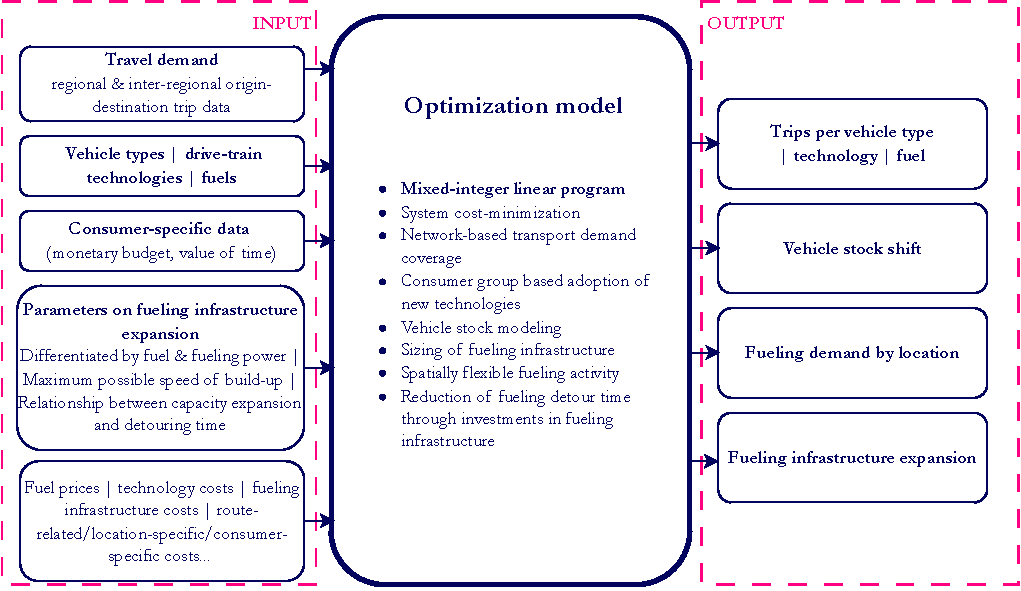
\includegraphics[width=\textwidth]{graphics/flowchart_sep25.drawio.pdf}
        \caption{Overview on the input and output parameters of the optimization model and its core functionalities} \label{fig:overview_method}
    \end{figure}
\begin{table}[H]
\caption{Overview of integrated model functionalities drawn from state-of-the-art methodology. \textit{Fueling detour time} is written in cursive letters to imply that this model feature is not based in the existing state-of-the-art, and is, therefore, a novel extension. `-' implies that the included modeling feature is integrated without significant adaptations from the initial concepts. The listed sources are references to research papers that describe or apply these modeling approaches. }
\label{tab:state-of-the-art-method}
\resizebox{\textwidth}{!}{%
\begin{tabular}{lll}
\hline
Modeling feature                                                                                                         & State-of-the art references & Adoption/extension in this work                                                                                                                                           \\ \hline
\begin{tabular}[t]{@{}l@{}}Network design and transport \\ demand coverage\end{tabular}                                 &                      \citep{Yang01071998}          &      -                                                                                                                                                                     \\
\begin{tabular}[t]{@{}l@{}}Consumer groups of different income-class levels\\ and level of service measure\end{tabular} &  \citep{TATTINI2018265}, \citep{LUH2024122412}                          & \begin{tabular}[t]{@{}l@{}}-\end{tabular}                                                            \\
Vehicle stock modeling                                                                                                  &    \citep{Fridstrom2016}, \citep{MARTIN2024132882}                        &                                        -                                                                                                                                   \\


\begin{tabular}[t]{@{}l@{}}Sizing of different types of fueling \\ infrastructure\end{tabular}                          &    \citep{BAKKER2025104076}, \citep{luh2022behavior}                           & \begin{tabular}[t]{@{}l@{}}-\end{tabular} \\
\begin{tabular}[t]{@{}l@{}}Spatially flexible allocation of \\ fueling activity\end{tabular}                            &  \citep{WANG2025135452}                         &      -                                                                                                                                                                     \\
\textit{Fueling detour time}                                                                                                     &                            &  \begin{tabular}[t]{@{}l@{}}Consideration of the time required to\\reach closest charging station\end{tabular}                                                                                                                                                       \\ \hline
\end{tabular}%
}
\end{table}   

        


    \subsection{Linear program} \label{sec:math_model}
    % Please add the following required packages to your document preamble:
% Please add the following required packages to your document preamble:

% Note: It may be necessary to compile the document several times to get a multi-page table to line up properly
% Please add the following required packages to your document preamble:
% \usepackage{longtable}
% Note: It may be necessary to compile the document several times to get a multi-page table to line up properly
 In the following, we elaborate on the mathematical formulation of the model functionalities that are extensions from state-of-the-art methodologies. The remaining constraints are to be found in the \ref{sec: extended_math_form}. Table \ref{tab:nomenclature_main_sel} contains the relevant nomenclature used in the following equations.
 \begin{scriptsize}
\begin{longtable}{llll}
\caption{Nomenclature (selection).}
\label{tab:nomenclature_main_sel}\\
\hline
Sets and indices                         & Description                                                          &         &               \\ \hline
\endfirsthead
%
\endhead
%
\hline
\endfoot
%
\endlastfoot
%
$y \in \mathcal{Y}$                      & year                                                                 &         &               \\

$u \in \mathcal{U}$                      & consumer group                                                           &         &               \\
$p \in \mathcal{P}$                      & trip purpose                                                         &         &               \\
$r \in \mathcal{R}_p$                      & trip between origin-destination (OD) pair for a specified purpose                                        &         &               \\
$k \in \mathcal{K}$                      & travel paths                                                         &         &               \\

$e \in \mathcal{E}$                      & geographic location                                                  &         &               \\
$v \in \mathcal{V}$                      & type of vehicle                                                      &         &               \\
$t \in \mathcal{T}_v$                      & drive-train technology fueled by a specific fuel                     &         &               \\
$g \in \mathcal{G}$                      & year that vehicle was introduced to market                           &         &               \\
$l \in \mathcal{L}$                      & types of fueling infrastructure (by capacity) &         &               \\
$i \in \mathcal{I}_l$ &  \multicolumn{3}{l}{index for detour time reduction potential for type of fueling infrastructure $l$ }\\
$\mathcal{Y}^{exp}$                      & set of years of investment decisions                                 &         &               \\
$\mathcal{K}_{e}$                      &   set of paths that go through edge $e$                               &         &               \\
$\mathcal{L}^{not home}$ &
  \multicolumn{3}{l}{fueling infrastructure that is not allocated at home of vehicle owner} 
   \\
   
   $\mathcal{L}^{home}$ &
  fueling infrastructure that is allocated at home of vehicle owner &
   &
   \\
   $\mathcal{L}_{tk}$ &  \multicolumn{3}{l}{types of infrastructure by drive-train technology and availability for travel path} \\
   $\mathcal{E}_{kl}$ & geographic location along travel path and available fueling type & & \\
   $S^u_j$ & \multicolumn{3}{l}{\begin{tabular}[t]{@{}l@{}}$ = \{ y_m \in Y | j \in [m, m + \tau_u -1]\}, m=1, ..., |Y| -\tau _u +1 $ \\ subsets of time periods for which a monetary budget is defined by consumer group\end{tabular}}   \\   
   \\\hline
Decision variables                       &                                                                      & Unit    &               \\ \hline
$f_{yurkvtg}$                           & number of person-trips                                                      &   -      & $[0,\infty[$  \\
\textbf{$h_{yurkvtg}$}                  & number of vehicles                                                   &      -   & $[0, \infty[$ \\
$h^{+}_{yurkvtg}$                       & newly purchased vehicles                                             &    -     & $[0,\infty[$  \\
$h^{-}_{yurkvtg}$                       & number of vehicles leaving the vehicle stock                         &   -      & $[0, \infty[$ \\
$s_{yurkvtgle}$                         & energy fueled                                                        & kWh     & $[0, \infty[$ \\
$n_{yurkvtgle}$               & number of fueling vehicles                                           &         & $[0, \infty[$ \\
\replaced{$b_{yurkvtle}$}{$b_{yiel}$} &
  \begin{tabular}[t]{@{}l@{}}fueling detour time to reach closest available public charging \\ infrastructure\end{tabular} &
  h &
  $[0, \infty[$ \\
$w_{yeli}$ &
  \begin{tabular}[t]{@{}l@{}}binary decision variable indicating whether detour reduction $i$ is\\ active\end{tabular} &
   - &
  $\{ 0, 1\}$ \\
$z_{yrkvtle,i}$ &
  decision variable substituting the multiplication $b* w$ &
  h &
  $[0, \infty[$ \\
$q^{+,\mathrm{fuel\_infr, home}}_{yrte}$ & added fueling infrastructure at home                                 & kW      & $[0,\infty[$  \\
$q^{+, \mathrm{fuel\_infr}}_ {ytle}$               & added fueling infrastructure                                         & kW      & $[0, \infty[$ \\
$q^{\Delta +, \mathrm{fuel\_infr}}_ {ytle}$               & \begin{tabular}[t]{@{}l@{}}relative difference of fueling capacity expansion to fixed capacity \\ size values $cap$\end{tabular}                                          & kW      & $[0, \infty[$ \\
$\mathrm{budget}^{+}_{yur}$              & budget overrun                                                       & \euro   & $[0, \infty[$ \\
$\mathrm{budget}^{-}_{yur}$              & budget underrun                                                      & \euro   & $[0, \infty[$ \\ \hline
Parameters                               &                                                                      &         &               \\ \hline
$\mathrm{LoS}$                           & level of service                                                     & h       &  $[0, \infty[$             \\
$\mathrm{VoT}$                           & value of time                                                        & \euro/h &  $[0, \infty[$             \\
$\gamma_l$                               & factor between annual peak hour and total annual demand                                                                &     \%    &   $[0, 100]$            \\
$Q^{\mathrm{fuel_infr, not home}}_{urte}$         & Initial fueling infrastructure at home                               & kW      &     $[0, \infty[$          \\
$Q^{\mathrm{fuel_infr, home}}_{urtle}$                       & Initial fueling infrastructure                                        & kW      &     $[0, \infty[$          \\
$\alpha_{iel}$                           & reduction $i = 1, \dots, I$ of detour time                           & \%      &        $[0, 100]$       \\
$cap_{iel}$                           & \begin{tabular}[t]{@{}l@{}}fixed lower bounds for capacity which tie to a reduction of\\ detour time of $\alpha_{i}$  \end{tabular}                         & kWh      &          $[0, \infty[$     \\
$\tau^u$                                 &  \begin{tabular}[t]{@{}l@{}}number of years between consecutive vehicle purchase decisions, \\representing the vehicle replacement period.       \end{tabular}                                  &   a      &        $[0, \infty[$        \\
$\beta$                                 & relative threshold for budget under- or overrun                                         &       \%  &   $[0, 100]$             \\

$B^{\mathrm{init}}_{el}$                          & initial detour time                                                  &      h   &   $[0, \infty[$           \\

$L_{k}$                                  & length of path                                                       & km      &     $[0, \infty[$          \\ 
$C^{\mathrm{CAPEX}}_{yvtg}$  & expenditure costs for vehicles & -&  $[0, \infty[$\\
$\mathrm{Budget}_u$ & monetary budget of consumer group&  \euro/trip & $[0, \infty[$\\ \hline
\end{longtable}
\end{scriptsize}

        \subsubsection*{Objective function}
        The objective function comprises costs for the vehicle stock (${C}^{\mathrm{vehicle\_stock, total}}$), required fueling (${C}^{\mathrm{fueling, total}}$), costs for fueling infrastructure (${C}^{\mathrm{infrastructure, total}}$), and intangible costs (${C}^{\mathrm{intangiblecosts, total}}$) as well as penalty costs (${C}^{\mathrm{\replaced{paneltycosts}{penaltycosts}, total}}$) that are introduced here to \replaced{penalize the}{leverage} overrun or the underrun of monetary budgets of consumers. The objective function is defined as follows: 
         \begin{flalign} \label{equ:obj_fun}
            \begin{split}
                \underset{f,h,h^{+}, h^{-},s,n,b,w, z,q^{+}, \textrm{budget}^+, \textrm{budget}^-}{minimize} z = {C}^{\mathrm{vehicle\_stock, total}} + {C}^{\mathrm{fueling, total}} \\\\ +  {C}^{\mathrm{infrastructure, total}} +{C}^{\mathrm{intangiblecosts, total}}  +{C}^{\mathrm{penaltycosts, total}}
            \end{split}
         \end{flalign}

        The vehicle stock is sized to cover all car trips and the required fueling activity is allocated among the visited geographic \replaced{locations}{features} of a car trip and different fueling infrastructure types. The latter may imply, for example, fueling infrastructure \deleted{that is }installed at home or work, or public fueling infrastructure. 
        
        \subsubsection*{Sizing of different types of fueling infrastructure} Fueling infrastructure is expanded for each investment period, $y' \in \mathcal{Y}^{exp}$, and sized based on an assumed factor which represents the ratio between the annual demand peak and the annual total demand, $\gamma_l$. We differentiate here between fueling infrastructure of which the availability is independent from the particular trip ($\mathcal{L}^{\mathrm{not home}}$) and those that are dependent on it as this fueling infrastructure is installed at home ($\mathcal{L^{\mathrm{home}}}$). 
            \begin{flalign} \label{equ:cap_fuel_e}
                \begin{split}
                        Q^{\mathrm{fuel\_infr}}_{tle} + \sum_{y' \in \mathcal{Y}^{\mathrm{exp}}_y} q^{+, \mathrm{fuel\_infr}}_{y'tle} \geq \gamma_l\sum_{r \in \mathcal{R}} \sum_{k \in \mathcal{K}_e} \sum_{u \in \mathcal{U}} \sum_{g \in \mathcal{G}}  s_{yurkvtgle} : \forall y,t,e,l \in \mathcal{L}^{\textrm{not home}} \\
                        Q^{\mathrm{fuel\_infr}, \textrm{home}}_{urtle}  + \sum_{y' \in \mathcal{Y}^{\textrm{exp}}_y} q^{+, \mathrm{fuel\_infr, home}}_{y'urtle} \geq \gamma_l\sum_{k \in \mathcal{K}_e} \sum_{g \in \mathcal{G}}  s_{yurkvtgle} : \forall y,u,t,r,e, l \in \mathcal{L}^{\mathrm{home}} \\
                \end{split}
            \end{flalign}
        $s$ refers to the annual fueling demand.

        \subsubsection*{Consumer groups by different income-class levels and level of service measure} The intangible costs (${C}^{\mathrm{intangiblecosts, total}}$) represent non-monetary costs that are monetized in the objective function by \replaced{weighting them}{being weighted} with the consumer-group-dependent VoT. The non-monetary costs refer \added{to }in particular \deleted{to }the total travel time associated with different vehicle types and drive\deleted{-}train technologies, i.e., the level of service:
        \begin{flalign}
            \begin{split}
                {C}^{\mathrm{intangiblecosts, total}} =  \sum_{y,u,r,k,v,t,g} \mathrm{VoT}_{u} * \bigg(\mathrm{LoS}^{f}_{ykvt} * f_{yurkvtg} + \sum_l b_{yurkvtle}\bigg)
            \end{split}
        \end{flalign}

        $f$ is the number of person-trips. The parameter $\mathrm{LoS}$ is the level of service, i.e\added{,} total travel time, associated with a vehicle type and drive\deleted{-}train technology for a trip\deleted{ is}:

        \begin{flalign}
            \begin{split}
                \mathrm{LoS}^f_{ykvt} = \frac{L_k}{\mathrm{speed}_{vt}} + \mathrm{fueling\_time}_{ykvt} \quad :\forall y,k,v,t
            \end{split}
        \end{flalign}

        Decision variable $b$ is the fueling detour time, \replaced{i.e.,}{being} the additional travel time.  

        Monetary budgets vary by consumer group. These are defined \replaced{by}{via} the temporal frequency of car purchases, i.e.\added{,} every $\tau$ years. The budget constrains expenditures for vehicles and fueling infrastructure installed at home, which is the left side of these constraints:  

        % \begin{flalign} \label{equ:monetary_budget_plus}
        %     \begin{split}
        %          \sum_{y \in \mathcal{Y}^i} \left( C^{\mathrm{CAPEX, vehicle}}_{yvtg} * h^{+}_{yr} + C^{\mathrm{CAPEX, fuel\_infr} }\sum_{y' \in \mathcal{Y}^{\textrm{exp}}_y} q^{+, fuel\_infr, \textrm{home}}_{yrte} \right) \leq Budget_{u} * f * \tau_j +  \sum_{y \in \mathcal{Y}^i} \mathrm{budget}^{+}_{yur}\\ \quad : \forall y,u,r,i
        %          \end{split}
        % \end{flalign}

        \begin{flalign} \label{equ:lower_constraint}
            \begin{split}
                \sum_{y \in \mathcal{S}^u_j} \left( \sum_{vtg}C^{\mathrm{CAPEX}}_{yvtg} * h^{+}_{yurvtg} + \sum_{tl}\sum_{y' \in \mathcal{Y}^{\textrm{exp}}_{y'}} q^{+, \mathrm{fuel\_infr, home}}_{yurtle} \right) \\ \leq \beta *\tau_u * \mathrm{Budget}_{u} * \sum_{kvtg} f_{yurkvtg}    + \sum_{y \in \mathcal{S}^u_j} \mathrm{budget}^{+}_{yur}  \quad : \forall y,u,r,j
            \end{split}
        \end{flalign}
        \begin{flalign} \label{equ:upper_constraint}
            \begin{split}
               \sum_{y \in \mathcal{S}^u_j} \left( \sum_{vtg}C^{\mathrm{CAPEX}}_{yvtg} * h^{+}_{yurvtg} + \sum_{tl}\sum_{y' \in \mathcal{Y}^{\textrm{exp}}_{y'}} q^{+, \mathrm{fuel\_infr, home}}_{yurtle} \right) \\ \geq \beta *\tau_u * \mathrm{Budget}_{u} * \sum_{kvtg} f_{yurkvtg}    - \sum_{y \in \mathcal{S}^u_j} \mathrm{budget}^{-}_{yur}  \quad : \forall y,u,r,j
            \end{split}
        \end{flalign}
        
        

        Equation \ref{equ:lower_constraint} expresses the lower limit for the expenditures, which relate to the investments in new vehicles (left \added{hand-}side of the equation). Equation \ref{equ:upper_constraint} imposes an upper limit on \replaced{these expenditures}{this}. A threshold for the budget is included with the factor $\beta$. Budget underrun and overrun, $\mathrm{budget}^{-}_{yur}$ and $\mathrm{budget}^{+}_{yur}$\added{,} are decision variables that are penalized in the objective function and leveraged with a factor in the term ${C}^{\mathrm{paneltycosts, total}}$ (Equation \ref{equ:obj_fun}).
        
        \subsubsection*{Mixed-integer extension: Fueling detour time} 
        We introduce lumpiness in the sizing of the infrastructure\added{,} which is expressed by: 

        \begin{flalign}
            \begin{split}
                Q^{\mathrm{fuel\_infr}}_{tle} + \sum_{y' \in \mathcal{Y}^{\mathrm{exp}}_y} q^{+, \mathrm{fuel\_infr}}_{y'tle} = \sum_i w_{yiel} * cap_{iel} + q^{\Delta+, \mathrm{fuel\_infr}}_{y'tle} : \forall y,t,e,l \in \mathcal{L}^{\textrm{not home}}\\
                \sum_i w_{yiel} = 1 \quad : \forall y, e, l  \in \mathcal{L}^{\textrm{not home}}
            \end{split}
        \end{flalign}
     
        $q^{\Delta+, \mathrm{fuel\_infr}}_{y'tle}$ is \deleted{here }a continuous variable that expresses the relative difference in capacity to the fixed capacity values\deleted{,} $cap_{iel}$. 
        The lumpiness is introduced via the binary variable $w$ and ties \deleted{the }fueling infrastructure expansion to the reduction of detour\deleted{ing} time. 
        
        The fueling detour time is explicitly defined only for fueling types \deleted{that are }not allocated at home, for $l \in \mathcal{L}^{\textrm{not home}}$. Based on an assumed fueling detour time $B^{\textrm{init}}$ that is initially needed to reach the nearest fueling station for refueling, we model the relative reductions \replaced{of}{in} the detour\deleted{ing} time that \replaced{directly result}{results directly} from the expansion of the fueling infrastructure capacities. The decision variable $b$ represents the total annual detour time of all vehicles by trip for this vehicle type, drive\deleted{-}train technology fueling using the type of fueling infrastructure $l$ at the geographic location $e$. \replaced{This expresses as follows:}{We express this in the following way:}
        \begin{empheq}[left={ b_{yiel} =\empheqlbrace}]{equation}
          \begin{aligned}
              & B^{init} * (1-\alpha_{iel}) * \sum_{u,r,v,g} \sum_{k \in \mathcal{K}^{e}}\sum_{t \in \mathcal{F}^e} n_{yurkvtge}& & \text{if } w_{yiel} = 1\\[1ex]
              & 0 & & \text{if }  w_{yiel} = 0
          \end{aligned}
        \end{empheq}


        $\alpha_i^{-}$ represents the $i$th reduction of the detour time in percentage at fueling capacity $cap_i$. 
        \added{For better understanding of the computation of this equation, we provide the following example: At location $e$, there are 1000 vehicles charges (expressed by $\sum_{u,r,v,g} \sum_{k \in \mathcal{K}^{e}}\sum_{t \in \mathcal{F}^e} n_{yurkvtge}$). Due to the total installed public charging capacity at location $e$, the reduction $\alpha_{(i=7)e}$ is active which reduces the initial detouring time, $B^{init}$ by 80\%. $B^{init}$ equals 60 minutes. Based on this, the total detouring time at this location is $b = 60\mathrm{min} * (1-0.8) * 1000 = 120,000 min$.}
    
        
        
    \subsection{Numerical case study} \label{sec:numerical_case_study}

        \subsubsection{Basque Country}

        The geographic extent of \replaced{this}{the} analysis of this paper is the autonomous community Basque Country (in Spanish: \textit{País Vasco}, NUTS code: ES21). This region is located in the North of Spain. The current passenger car vehicle stock is in the magnitude of 1\replaced{.}{,}08 Mio. (2022) \citep{eurostat_transport2024}. In 2023, the electrification rate of the passenger car fleet was at 0.05\% \citep{eurostat_zev_2024}. The Basque Country is classified as a NUTS-2 region in the EV NUTS classification scheme \citep{eurostat_nuts} and consists of three NUTS-3 regions: Araba/Álava\footnote{For the readability of the article, we\deleted{ will} refer to the region by its Basque language, Araba.} (ES211), Guipuzcoa (ES212), \replaced{Bizkaia}{Bizcaya} (ES213). Figure \ref{fig: scenario_design} displays the relative geographic allocation of the regions and of the capital cities. For RQ1, we represent the NUTS-2\added{ region} as one node.
        For RQ2, we \replaced{derive}{deduct} a graph-based conceptualization with three nodes representing each of the NUTS-3 regions and three edges representing the transport connections between neighboring regions.    

 

        \paragraph*{Pre-processing of travel demand data}
            \paragraph*{Origin-destination data}
            We use the modeled passenger car trips by ETISplus data\deleted{ }base \citep{ETISplus_233596} which hold\added{s} information about: origin, destination zones (NUTS-3 level \citep{eurostat_nuts}), trip purposes, as well as route lengths and shortest-path route information for trips between all regions. 
            A subset \replaced{including}{that includes} NUTS-3 regions of the Basque Country is extracted\deleted{ from this}. We further exclude all trips that go beyond the border of the case study area. This corresponds to the selection of 99\% of all trips \deleted{that }originat\replaced{ing}{e} from there. Based on this, we set the system boundaries of the analysis equal to the boundaries of the Basque Country.

            The ETISplus data \replaced{were}{has been} calibrated for transportation demand in 2010. To consider the growth in passenger car trips since then, we use the relative growth of the passenger car fleet since then \citep{arval2023fleet}. The subsequent growth of the travel demand until 2050 is extrapolated based on historic GDP growth since 2020 \citep{statistaGDPSpain}.
           
            Trips are categorized \replaced{by}{for} the following purposes: \textit{Business}, \textit{Private}, \textit{Vacation}, and \textit{Commuting}. Trip purposes of the category \textit{Business} are taken into account in the sizing of fueling infrastructure, but are not assigned to explicit consumer groups of different income levels. \textit{Private} trips are defined as non-business trips with a duration \added{of }up to four days, while \textit{Vacation} \replaced{refers to}{labels} trips that take more than four days. \textit{Commuting} includes daily trips for working and studying purposes. Figure \ref{fig:nb_trips} displays the initial data trip count by purpose for local trips, i.e. within a NUTS-3 region, and inter-regional trips between NUTS-3 regions within the Basque \replaced{C}{c}ountry.
            
            

            
            \begin{figure}[H]
                \centering
                    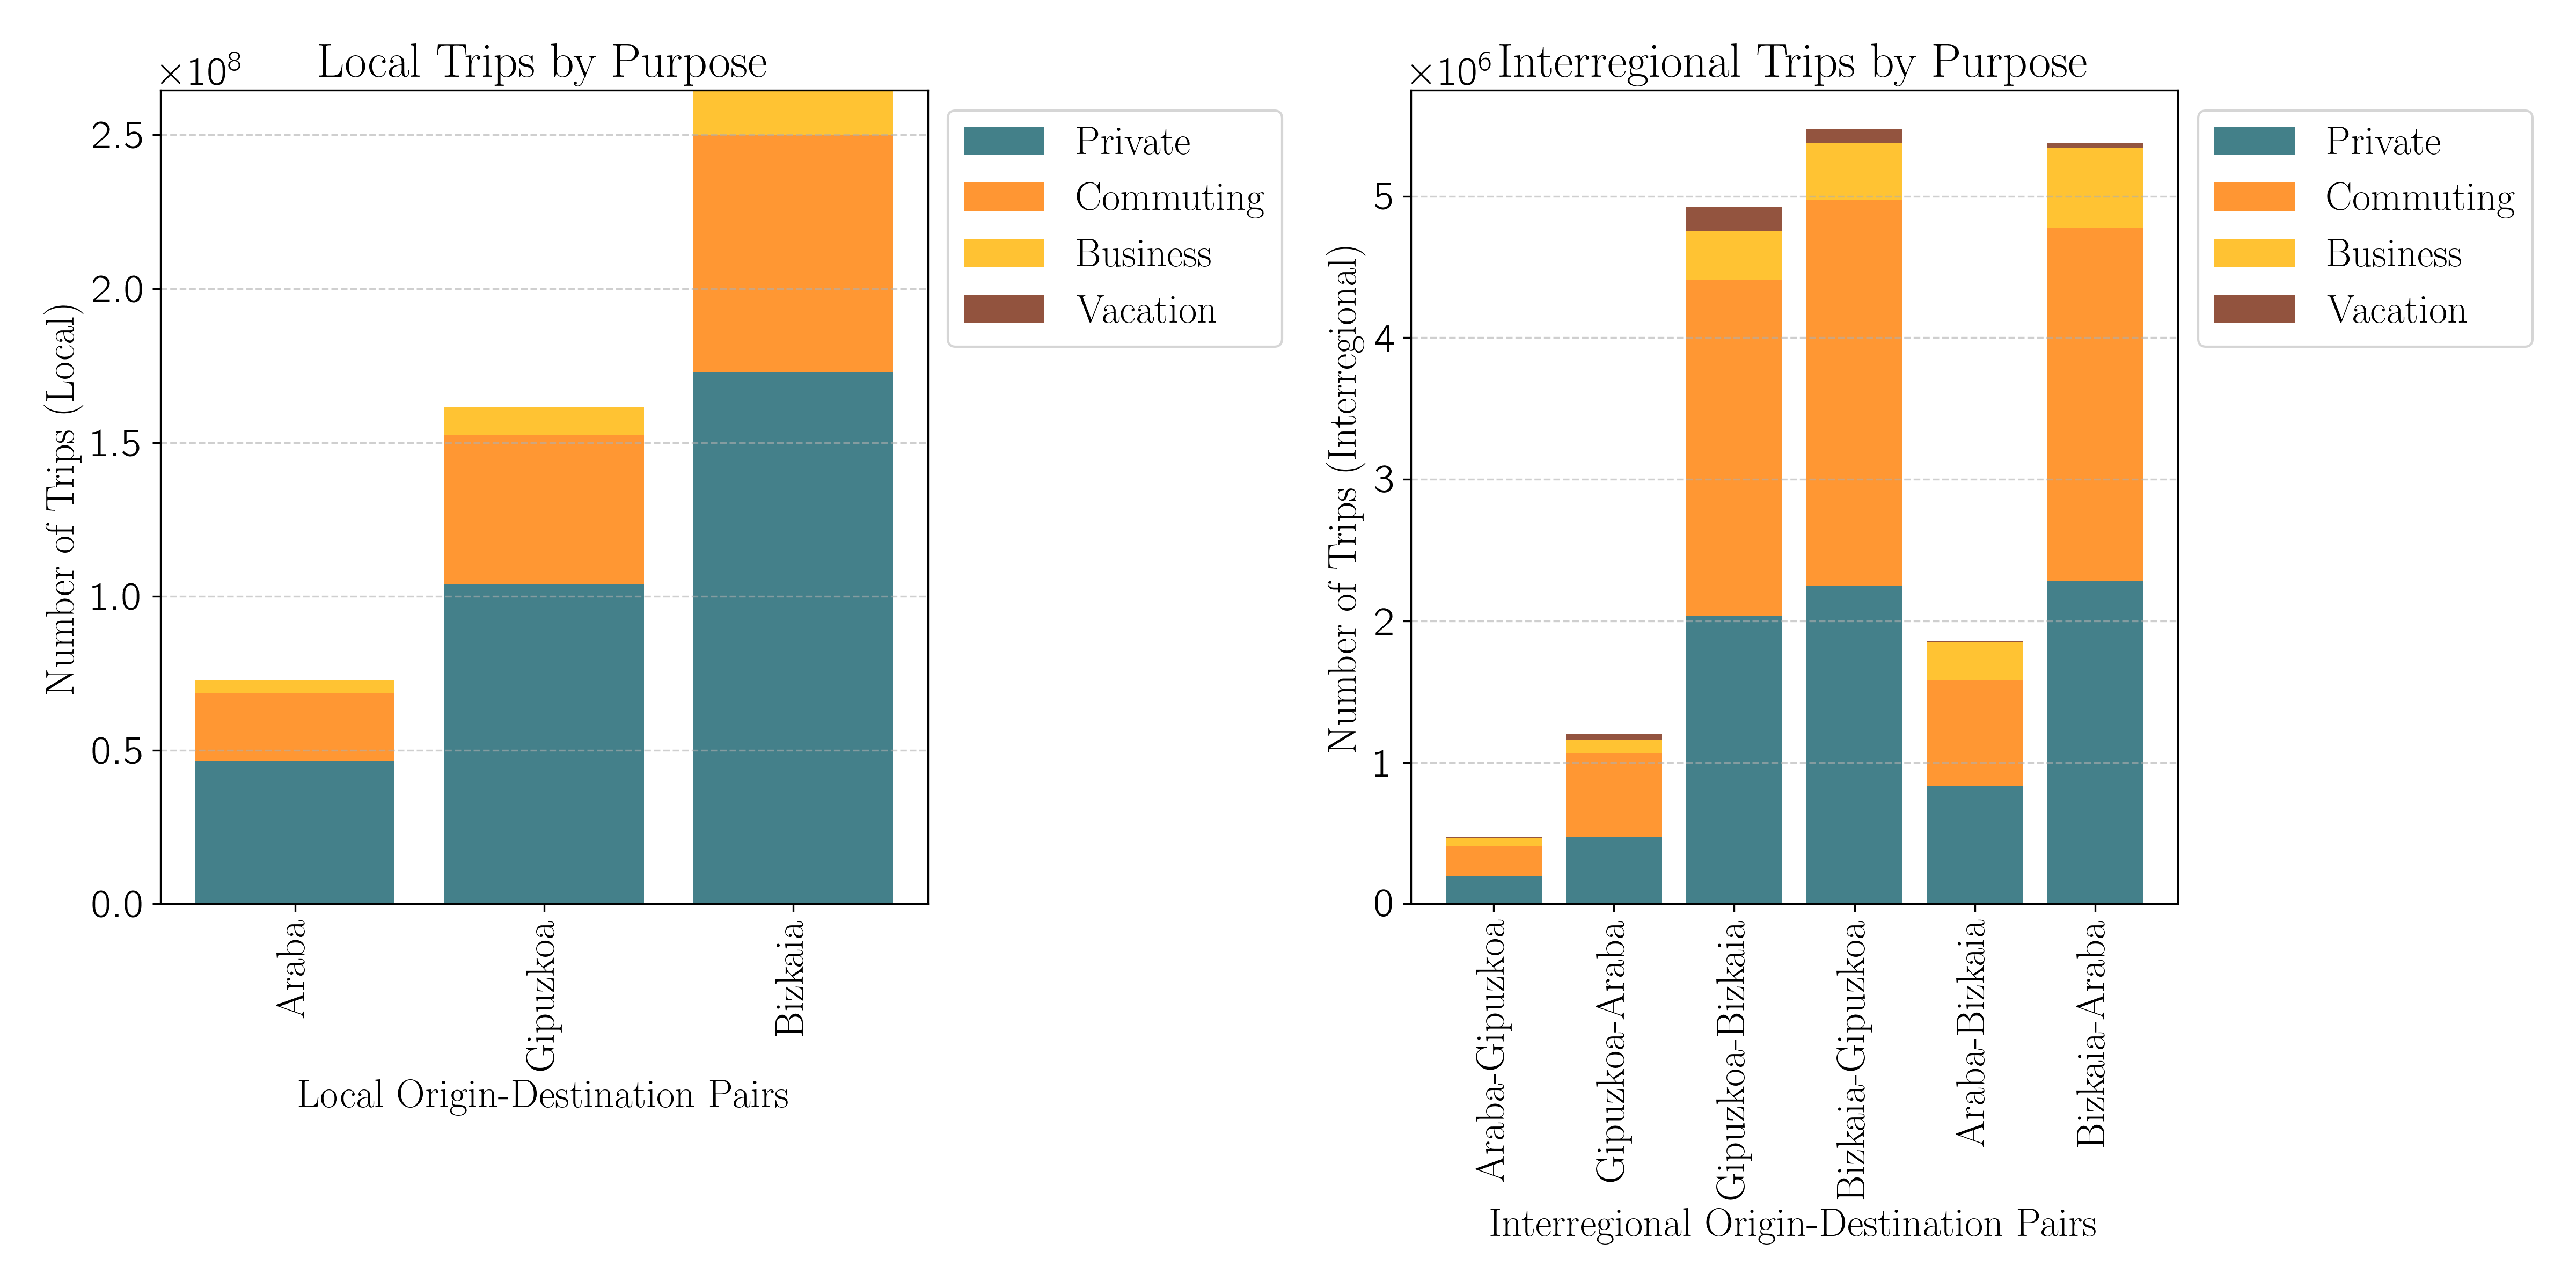
\includegraphics[width=\textwidth]{graphics/stacked_bar_plot_trips_subplots_with_separate_y_axes.png}
                    \caption{Passenger car trips by purpose: Within a NUTS-3 region (\textit{left}) and between NUTS-3 regions (\textit{right})}
                \label{fig:nb_trips}
            \end{figure}
       
            
        In the underlying data set by ETISplus, route lengths are given for the connections between NUTS-3 regions but not for trips within a region. To compensate for this missing information, we perform the assignment of route lengths (see Table \ref{tab:path_length_assumptions}). More details on the assumptions made in this process are in the Appendix of the manuscript (see Appendix \ref{sec: extended_math_form}). 
        
       \begin{longtable}{@{}llcrr@{}}
        \caption{Path lengths assigned to trips within a region (same origin and destination on NUTS-3 level)}
        \label{tab:path_length_assumptions}\\
        \toprule
              &                          & \multicolumn{3}{c}{Average trip length (km)} \\* \midrule
        \endfirsthead
        %
        \endhead
        %
        Region type & Share of total trips within a region & Private & \multicolumn{1}{c}{Commuting} & \multicolumn{1}{c}{Business} \\* \midrule
        Urban & \multicolumn{1}{r}{21\%} & \multicolumn{1}{r}{7.4}    & 10.4   & 13.0   \\
        Rural & \multicolumn{1}{r}{79\%} & \multicolumn{1}{r}{9.7}    & 17.1   & 23.2   \\* \bottomrule
        \end{longtable}
        \paragraph*{Introduction of income-class specific parameters}
            
            \added{The key assumptions in the introduction of the income-class specific parameters is that the central difference in travel patterns by income class is the motorization rate, by monetary budget and home ownership \citep{tikoudis2024oecd246, CHATTERTON201830}}. The income classes are characterized by having different monetary budgets for the purchase of vehicles and different VoT values. We consider five different income classes: \textit{Very high income}, \textit{High income}, \textit{Medium \replaced{l}{h}ow income}, \textit{Low income} and \textit{Very low income} class, mirroring the income class classification of EUROSTAT via five quintiles \citep{eurostat_icw_metadata}. The most important pre\deleted{-}processing steps related to the income classes include the distribution of trips among them, the determination of monetary budgets and limitations for home-based charging infrastructure. 
            We, therefore, characterize the five consumer groups by the motorization rate, VoT, average monetary budgets for new vehicles, the frequency of vehicle purchase, and the share of home ownership. Assumptions for these are summarized in Table \ref{tab:income_class_ass}.
            
            
            \citet{Mattioli2023} define a relation between motorization rate and purchasing power on NUTS-2 region level, derived from EUROSTAT data. 
            We use this as a proxy to determine a relationship between the purchasing power standard (PPS) of the income class and the motorization rate, together with the average motorization rate in the Basque \replaced{Country}{community}. \replaced{This relationship is}{Which is}: $\textrm{Motorization rate} = 0.02 \times \textrm{PPS} + 79$.  The $\mathrm{VoT}$ parameter is reported to vary significantly based on the monetary budgets. We use the value used in the case study by \citet{TATTINI2018265} who apply these values in the context of a Danish case study. Due to the lack of published data for VoT values calibrated for different income classes in Spain or the Basque Country, we assume similar values for the present case study as found for Denmark and adapt these based on relative purchase power numbers\added{, applying the factor $\times (92/139)$} \citep{Eurostat_ilc_di02_2025}.
            
            % \paragraph*{Assigning vehicle trips to households of different income classes}
            % \begin{itemize}
            %     \item Distribution of income levels
            %     \item motorization by income level
            % \end{itemize}
            % Methodology for assigning income classes:
            % \begin{itemize}
            %     \item Assumption: household size is assumed constant among all income classes
            %     \item Assumption: mobility behavior (trip length and frequencies) are also constant through the income classes
            %     \item EUROSTAT gives the average disposable income per household for each income class 
            %     \item 
            % \end{itemize}
            % The resulting motorization rate by income class is displayed in Table \ref{tab:income_class_ass}.

                % Please add the following required packages to your document preamble:
                % \usepackage{booktabs}
                % Please add the following required packages to your document preamble:
                % \usepackage{booktabs}
                % \usepackage{graphicx}
                \begin{table}[H]
                \centering
                \caption{Overview on assumptions between the income classes}
                \label{tab:income_class_ass}
                \resizebox{\textwidth}{!}{%
                \begin{tabular}{@{}lrrrrrr@{}}
                \toprule
                \textit{Income class} &
                \textit{Purchase Power Standard} &
                \begin{tabular}[c]{@{}c@{}}\textit{Motorization rate} \\ \textit{(nb. of veh/1000)}\end{tabular} &
                \begin{tabular}[c]{@{}c@{}}\textit{Value of Time} \\ \textit{(\euro/h)}\end{tabular} &
                \begin{tabular}[c]{@{}c@{}}\textit{Average monetary budget} \\ \textit{ over 10 years (\euro)}\end{tabular} &
                \textit{Purchase frequency (a)} &
                \textit{Assumed home ownership} \\ \midrule
                Very low    & 10081 & 338  & 6.60  & 4160  & 10 & 30\%  \\
                Low         & 19685 & 425  & 12.77 & 9282  & 8  & 55\%  \\
                Medium low & 27932 & 500  & 18.93 & 13910 & 6  & 85\%  \\
                High        & 37910 & 599 & 25.10 & 18824 & 4  & 100\% \\
                Very high   & 61086 & 800  & 31.27 & 26545 & 2  & 100\% \\ \bottomrule
                \end{tabular}%
                }
                \end{table}
                
                A statistic for \added{the }UK details expenditures for \deleted{the }purchases \citep{statista2023newcars} \citep{ons2024vehicle}, displaying an approximately linear relationship between level of income and expenditure for purchases, among with how much is spend on the primary market. Based on this, we determine the monetary budgets for a new vehicle from the primary market for the \textit{Very high}, \textit{High} and \textit{Medium High} income class, while we use the vehicle purchase price from the secondary market for the budget quantification of income class levels \textit{Low} and \textit{Very low}. \added{Home ownership is extrapolated from the average Spanish home ownership rate reported in \citep{statista_homeowners_spain}.} 


                



 \subsubsection{Drive\deleted{-}train technologies and fuels}
        
            When it comes to the selection of the drive\deleted{-}train technologies, we simplify it to two options: fossil-fueled vehicles and plug-in battery-electric vehicles. In contrast to this choice, studies in the literature have included larger technology portfolios by considering different electric car technologies, such as hydrogen fuel-cell or hybrid plug-in electric. The reason for the limitation to two technologies is twofold: Plug-in battery-electric vehicles have been largely proven to be \replaced{cost-wise and environmentally the most viable}{cost-wise and environmentally the most viable}, with a promising outlook on further cost decreases \citep{GRUBE2021103110}. Therefore, most policies focus on supporting this technology. We reduce the \deleted{used }fuels\added{ used} to \textit{fossil fuel}, including diesel and petrol, and electricity. Cost parameters for electricity are drawn from marginal costs for the energy system optimization for Spain performed with GENeSYS-MOD \citep{loffler2025european}. The average fuel price is based on \citep{MARTIN2023113637}. 
            Costs of the drive-train technologies are drawn from a detailed modeling of the manufacturing of all components by \citep{GRUBE2021103110}. We reduce the complexity of different car sizes to one representative vehicle type as related parameters to the choice of the car size - for example, household size, housing type \citep{jia2023preferences} - are not part of the modeling. Therefore, different sizes are excluded to avoid introducing a modeling bias due to insufficient complexity of the model. Table \ref{tab:assumptions_cost} summarizes all assumptions on cost parameters and sources. The cost assumptions are based on the work by \citet{GRUBE2021103110}  who have evaluated a wide range of different drive-train technologies for passenger cars and different passenger car sizes, including small, medium\added{,} and SUV. Here, we \replaced{derive}{deduct} the costs for an \textit{average}-sized vehicle by averaging the costs using weights that correspond to the magnitudes of the sizes in the current vehicle stock, assuming that this distribution would be constant throughout the optimization horizon. The data on different vehicle sizes represented in the statistic for different engine sizes in the Spanish vehicle stock \replaced{are}{is} retrieved from \citep{dgt2023}. 
            The costs for the maintenance are increased at a rate of 3\% per year for the first three years, and then by 10\% per year.
            

            To also allow for purchases from the second-hand vehicle market, purchasing options for vehicles of older generation are allowed for. For each technology, we introduce three groups of older vehicles with decreased investment costs but higher costs for maintenance and operation. The technological performance of vehicles available on the second-hand market is a function of their counterpart on the first-hand market and their average age. These three age-groups are: \textit{1-5}, \textit{6-10} and \textit{11\deleted{ }+ years}. The maximum lifetime of a vehicle is set to 25 years. An initial vehicle\added{ stock} with vehicles of different ages is assumed based on data from \citep{dgt2023}. The cost for vehicles on the second-hand market are calculated assuming a 65\% drop in resale price after the first year and after this, an annual 10\% cost decrease. The maintenance costs follow the annual increase in number as described above. 
            
            % Please add the following required packages to your document preamble:
% \usepackage{booktabs}
% Please add the following required packages to your document preamble:
% \usepackage{booktabs}
\begin{table}[]
\centering
\caption{Overview of a selection of assumed parametrization for passenger cars of battery-electric vehicles (BEV) and fossil-fueled internal-combustion engine vehicles (ICEV).}
\label{tab:assumptions_cost}
\begin{tabular}{@{}lrrrl@{}}
 \toprule
                                         & \multicolumn{1}{c}{2025} & \multicolumn{1}{c}{2035} & \multicolumn{1}{c}{2045} & Reference \\ \midrule
\multicolumn{5}{l}{\textbf{BEV (first-hand market)}}                                                                                  \\ \midrule
CAPEX (\euro)                                & 18,000                   & 16,100                   & 15,200                   &   \citep{GRUBE2021103110}        \\
fuel costs (\euro/kWh)                       & 0.05                     & 0.03                     & 0.03                     &    \citep{loffler2025european}       \\
Specific consumption (kWh/100km)         & 16.9                     & 13.4                     & 12.7                     &      \citep{GRUBE2021103110}     \\
Battery capacity (kWh)                   & 56                       & 69                       & 70                       &      \citep{GRUBE2021103110}     \\ \midrule
\multicolumn{5}{l}{\textbf{ICEV (first-hand market)}}                                                                                 \\ \midrule
CAPEX (\euro)                                & 12,000                   & 12,800                   & 13,200                   &   \citep{GRUBE2021103110}        \\
fuel costs (\euro/kWh)*                      & 0.08                     & 0.12                     & 0.18                     &      \citep{GRUBE2021103110}     \\
Specific consumption (kWh/100km)         & 58.1                     & 44.9                     & 36.9                     &      \citep{GRUBE2021103110}     \\
carbon price (\euro/tCO2) & 52                       & 113                      & 250                      &     \citep{loffler2017designing}      \\ \midrule
\multicolumn{5}{l}{\textbf{Charging infrastructure}}                                                                                  \\ \midrule
Level II: CAPEX (\euro/kW)                             & \multicolumn{3}{c}{108}                                                        &         \citep{Lanz2022}  \\
DCFC: CAPEX (\euro/kW)                             & \multicolumn{3}{c}{350}                                                        &  \citep{Lanz2022}         \\
OPEX                      & \multicolumn{3}{c}{30\% of CAPEX}                                                         &           \\ \midrule
\multicolumn{5}{l}{*without carbon pricing}                                                                                          
\end{tabular}
\end{table}
        \subsubsection{Types of charging infrastructure}
            For fossil-fueled vehicles, we assume that the fueling infrastructure with sufficient capacities has been established. Therefore, for combustion-engine passenger\added{ cars}, no expansion of the fueling infrastructure is required. 
    
            For charging infrastructure, we introduce four different types: Home (Level II), Workplace (Level II), Public slow (Level II)\added{,} and Public fast (DCFC) (based on \citep{LAMONACA2022111733}). Tables \ref{tab:charging_types} and \ref{tab:inits and restrictions} summarize relevant assumptions. The reduction \replaced{in}{for} fueling detour time is relevant for public infrastructure. In the case of fast charging (DCFC), the fueling time is considered \replaced{in addition}{additionally} to the level of service (similar as in the work by \citet{LUH2024122412}), while for the other types of infrastructure, we assume that there the charging is during typical down times of the vehicle and \deleted{is }therefore\added{ does} not impact\deleted{ing} the level of service. \added{Initial home charging capacity (40 MW in 2020) reflects the early adopter profile of BEV owners, who were predominantly homeowners with dedicated parking and charging infrastructure. This assumption is consistent with empirical findings that early BEV adopters had home charging access rates exceeding 90\% \citep{BARESCH2019388}.}

            
            

            \begin{table}[H]
            \caption{Overview on the introduced types of charging infrastructure and most important assumptions.}
            \label{tab:charging_types}
            \resizebox{\textwidth}{!}{%
            \begin{tabular}{lrlrcc}
            \hline
            Type of charging infrastructure & \multicolumn{1}{l}{Peak power level} & Location  & \multicolumn{1}{l}{Max. utilization rate}                                               & Fueling detour time  & Extra fueling time                                                                                                                                                                                                                                          \\ \hline
            Home (Level II)                & 11 kW                                & home      & 2\%    &                      &                                                                                                                             \\
            Workplace (Level II)           & 11 kW                                & workplace & 20\%            &   & \\                                             
            Public slow (Level II)              & 22 kW                                & public    & 25\%                                                           & $\times$                                                                               &                                                                                                                                                                       \\
            Public fast (DCFC)                            & 50 kW +                              & public    & 25\%                                                            & $\times$  & $\times$                                                                                                                                                                                                                                                              \\ \hline
            \end{tabular}%
            }
            \end{table}

            
            \begin{table}[H]
            \caption{Assumptions for the sizing of initial capacities and upper limits for the expansion of charging infrastructure.}
            \label{tab:inits and restrictions}
            \resizebox{\textwidth}{!}{%
            \begin{tabular}{lll}
            \hline
            Type of charging infrastructure & Sizing of initial charging infrastructure  & Limitation for capacity installation                                                                                                                                                                                                                                          \\ \hline
            Home (Level II)                 & \begin{tabular}[]{@{}l@{}} based on current observations in the share \\of charging processes at home chargers (88\%, \citep{BARESCH2019388}) \end{tabular} & \begin{tabular}[c]{@{}l@{}}Home charging infrastructure can be installed \\ in 30\% of owned homes.\end{tabular}                                                                                                                                                     \\
            Workplace (Level II)            & \begin{tabular}[]{@{}l@{}} based on current observations in the share \\of charging processes at workplace chargers (8.8\%, \citep{BARESCH2019388}) \end{tabular}& \begin{tabular}[c]{@{}l@{}}based on today's charging demand coverage at work \\and scaled by current total number of \\ passenger cars in the given region.\end{tabular} \\
            Public slow (Level II)              & current BEV-to-charging point ratio for public slow chargers \citep{eafo2024ev, eurostatZEV}                                                            & No upper limit                                                                                                                                                                                                                                                        \\
            Public fast (DCFC)                            & current BEV-to-charging point ratio for public fast chargers \citep{eafo2024ev, eurostatZEV}                                  & No upper limit                                                                                                                                                                                                                                                               \\ \hline
            \end{tabular}%
            }
            \end{table}

            \deleted{A maximum expansion of the entire charging capacity is imposed on basis of the planning power grid expansion for the Basque country (as reported in \citep{eve_basque_2025}). 6,000 MW additional grid capacity is planned to be installed by 2030 to meet the growing electricity demand in the industry, housing and e-mobility sector. We assume that 30\% of this capacity is reserved for e-mobility, which we derive from the relative share of total energy consumption \citep{eve_basque_energy_strategy_2030}}. \added{The maximum expansion speed of charging infrastructure is assumed to be 30\% which is in line with reported expansion speed by \cite{IEA2025GlobalEVOutlook}.} 

            To ensure that next to public slow charging, capacities for fast charging are installed to reduce range anxiety and enable recharge in cases of emergency (f.e. battery not sufficiently charged), we introduce a constraint imposing a minimum requirement for fast charging depending on the capacity installed for slow charging, which is set at the proportion of 2. This number is derived from the relative difference of the peak power level (the current value in Spain is 4.6 \citep{eafo2024ev}) .
            % These utilization of the infrastructure is introduced in the following way:
            %     \begin{itemize}
            %         \item $VoT \times \textrm{fueling time}$: The fueling time is only considered in the cases where fueling takes extra time. Here, this is considered when the charging needs to happen \textit{enroute} because of the travel distance being greater than the maximum driving distance.
            %         \item $VoT \times \textrm{detour timing}$. This gives a measure of the required extra time needed to reach the charging station; this refers to when the infrastructure is public. 
    
            %         \item \textbf{Availability (max. Cap.):} Home charging and work place charging have constraints on the maximum development of it. Home charging is mostly constrained by home ownership and workplace charging can be expanded to a certain limitation;
            %         \item \textbf{Cost allocation:} All capacities are leveraged with CAPEX and OPEX in the objective function. The home charging is a component that is added to the CAPEX of the vehicle purchase and is part of the budget constraint.
            %         \item \textbf{Capacity sizing:} This is part of the factor $\gamma$ which results from \textbf{peak hour assumption}, nb of vehicles that can be serviced a day. We assume that the relative number of minimum service is increasing for fast charging slightly throughout time. 
                    
            %     \end{itemize}
        
        


            % Please add the following required packages to your document preamble:
            % \usepackage{booktabs}
            % \usepackage{graphicx}
            % \begin{table}[H]
            
            % \begin{tabular}{@{}lllll@{}}\label{tab:cs_types}\caption{Considered charging infrastructure types varying by allocation and charging power.} 
            % \toprule
            % Type                 & Power  & Location  & Description of accessibility                   & Utilization \\ \midrule
            % Level II - home &
            %   10 kW &
            %   home &
            %   \begin{tabular}[c]{@{}l@{}}part of budget; only for homeownership possible/income class dependent?; \\ no detour time\end{tabular} &
            %   very low \\
            % Level II -public     & 22 kW  & public    & detour time;                                   & medium     \\
            % Level II - workplace & 10 kW  & workplace & no detour time; has limitation on installation & low        \\
            % DCFC                 & 50 kW+ & public    & detour time + time is money                    & medium     \\ \bottomrule
            % \end{tabular}%
            
            % \end{table}
            % Please add the following required packages to your document preamble:
% \usepackage{graphicx}


            % Initial public charging infrastructure is estimated based on the currently recorded charging-point-to-BEVs ratio which is \hl{\dots} [REF]. 
            % Initially existing charging infrastructure is estimated based on the following:
            % \begin{itemize}
            %     \item Public charging infrastructure is estimated based on the current charging-point-to-BEV ratio for Spain which is currently \hl{\dots} and is scaled for the Basque community based on the existing battery-electric vehicle stock. \hl{[REF]} gives information on the distribution for fast and slow charging.
            %     \item Home charging report a vehicle-to-point ratio for home chargers of 0.9. 
            %     \item Work place charging: No existing statistics on this can be found. We use the study of \citep{BARESCH2019388} as a baseline. It includes a current distribution of charging allocation between public, home and workplace charging - indicating an approx. 9\% of charging processes taking place at the workplace. We estimate the infrastructure based on this. 
            % \end{itemize}

            % \paragraph*{Restrictions of capacity expansion:}
            % \begin{itemize}
            %     \item Public charging infrastructure: no restriction
            %     \item Home charging: We constraint the maximum installation of home charging stations by the currently existing home ownership. We deduct this from EUROSTAT, and differ between urban and rural areas, assuming one charging station per house.
            %     \item Work place charging is assumed to be proportional to today's usage scaled by the future ev fleet. We assume it to be 50\%, based on that most workplaces do not have available charging stations and the charging station expansion would also be limited by the grid connection and parking place availability.
            %     %https://ec.europa.eu/eurostat/databrowser/view/ILC_LVHO01__custom_7139348/bookmark/table?lang=en&bookmarkId=82b32252-7125-4ec4-8a53-bf2d46622c4b
            % \end{itemize}
            

            
            % We assume an initial average detouring time by considering the following factors:
            % \textbf{Definition:} The average time that it takes to reach the closest not-occupied public charging station which is dependent on the following factors:
            % \begin{itemize}
            %     \item the type of charging station that is looked for (rapid/slow)
            %     \item existing infrastructure: rapid, slow, (possible assumption: this may be proportional to the available infrastructure); at workplace/POI/any public parking place; number of plugs per spot
            %     \item current utilization of the infrastructure (what are the chances that the very closest one is occupied?)
            % \end{itemize}
            
            % Potential sources for determining this are: 
            % \begin{itemize}
            %     \item Charging stations per vehicle ratio 
            %     \item EU directive: goal until 2030 to achieve ratio 1:10 (nb of charging stations to BEVs)
            % \end{itemize}
            
            % Under the assumption: urban situation is transferrable to sub-urban situation 
            
            % Assumptions:
            % \begin{itemize}
            %     \item Ratio between charging capacity and utilization is constant over all charging capacities
            %     \item 
            % \end{itemize}
            % The methodology of determining the current detouring time is the following:
            % \begin{enumerate}
            %     \item The number of existing public charging stations $N^{CS, public}$ is estimated via the ratio between exisiting number of charging points and the Number of BEVs ($N^{BEV}$), $\mu$:
            %         \begin{equation}
            %             N^{CP, public} = \mu \times N^{BEV}
            %         \end{equation}

            %     \item The number of vehicles charging at public charging stations is assumed via a known ratio $\rho$:
            %         \begin{equation}
            %             N^{BEV, public} = \rho \times N^{BEV}
            %         \end{equation}
            %     \item The vehicles serviced by one charging point a day is determined via the frequency of required recharging processes by number of days between the required charging processes, $N^{recharge}$:
            %     \begin{equation}
            %         N^{BEV\_day\_cp, public} = \frac{N^{BEV, public}}{N^{days, recharge}} 
            %     \end{equation}

            %     \item The probability that a charging station is occupied is then determined via the time of being typically serviced ($t^{service}$) and the time that one vehicle is serviced ($t^{session}$):
            %     \begin{equation}
            %         p_{occupied} = \frac{t^{session}}{t^{service}}
            %     \end{equation}

            %     \item To finally to determine the initial detouring time to the closest available charging station, we determine the number of charging points to ensure that changes are higher than 50\% that one is available:
            %         \begin{equation}
            %             n^{available} = \frac{\ln{0.5}}{\ln{p_{occupied}}}
            %         \end{equation}

            %     This is then multiplied by the average distance between two charging stations, $\overline{d^{cs}}$:
            %     \begin{equation}
            %         detour\_distance^{init} = \overline{d^{cs}} \times n^{available} 
            %     \end{equation}
                
            % \end{enumerate}
            % Initial charging infrastructure: % \textit{https://alternative-fuels-observatory.ec.europa.eu/sites/default/files/document-files/2024-05/Charging_ahead_Accelerating_the_roll-out_of_EU_electric_vehicle_charging_infrastructure.pdf}
            % densification is calculated based on constant capacities; but future vot is scaled with expecgted charging speeds 
            \subsection{Charging infrastructure roll-out scenarios} \label{sec:scenarios}

            Figure \ref{fig: scenario_design} illustrates the setup for analyzing different scenarios of the roll-out of public charging infrastructure. Illustrations 1 and 2 address the setup to answer RQ1: two expansion strategies are compared, the \textit{Concentrated} and the \textit{Distributed expansion}. For this, the case study area is considered as one NUTS-2 node, while for addressing RQ2, the area is modeled on NUTS-3 level with three nodes.
             \begin{figure}[H]
                        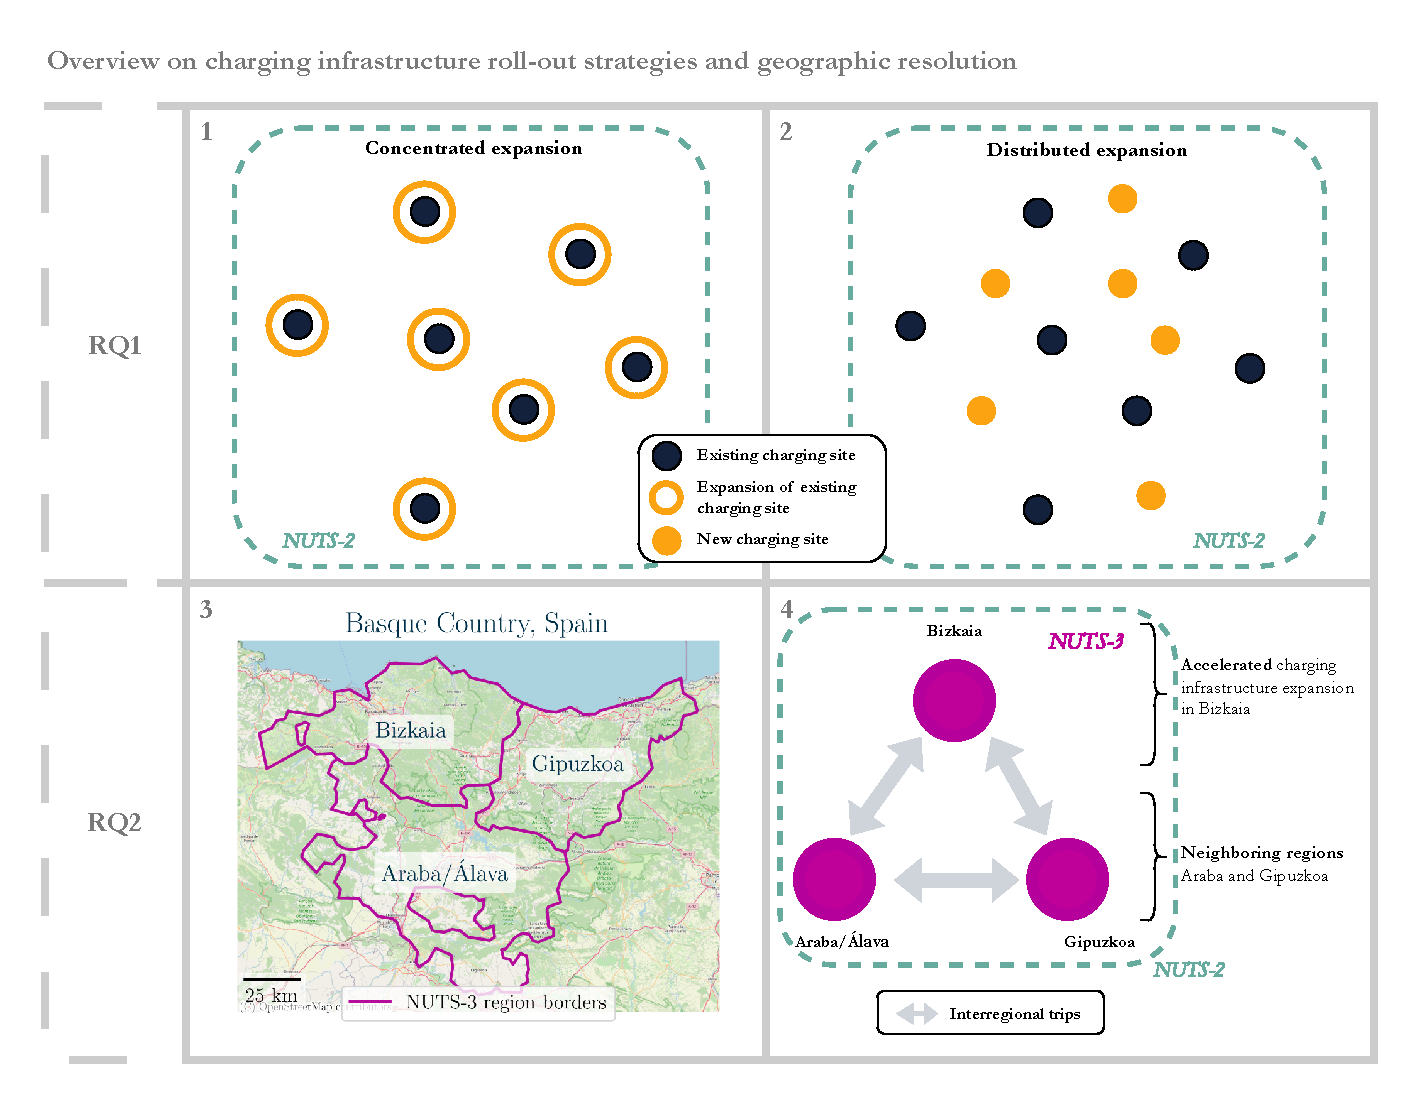
\includegraphics[width=\textwidth]{graphics/different_charging_infr_expansion_approaches.drawio.pdf} 
                        \caption{Overview of the scenario setups for the analysis. The top row (illustrations 1 and 2) displays the contrasting approaches to the densification of public charging infrastructure, addressing research question 1 (RQ1). In the bottom row, illustration 3 displays a map of the geographic area of Basque Country by its three NUTS-3 regions, together with the corresponding capitals. In illustration 4, it is implied which pace of charging infrastructure roll-out is assumed for the NUTS-3 regions --- addressing research question 2 (RQ2).} \label{fig: scenario_design}
                \end{figure} 
            \subsubsection*{Spatial densification (RQ1)}

                The spatial densification of charging infrastructure is addressed using the mixed-integer extension of the optimization model. For this, the trip data is accumulated to the NUTS-2 level. 
                
                To quantify the interaction between charging infrastructure investments and the detouring time required to reach the closest public charging station, a function between the average detouring time and installed charging capacities needs to be defined: 
                \begin{equation}
                    \alpha = g\left(q^{fuel\_infr, +}\right)
                \end{equation}
                $\alpha$ is the factor for the relative decrease of the fueling detour time and is a function of additionally built capacities. By formulating this function, we directly assume that the chargers are spatially evenly distributed \replaced{throughout the regions' road network}{relative to the allocation of BEV owners}. By doing this, we neglect the different degrees of urbanization and the option of allocating charging sites at points of interest, which would decrease detour\deleted{ing} time in reality. We do this with the premise that for a share of 100\% BEV penetration of the passenger car fleet, a spatially even distribution of charger availability is a necessity, to be equally accessible for all. Further, this assumption indicates that there are no malfunctions of charging points which could lead to extended detouring times.  
                The function $g()$ represents this relationship and varies for different charging infrastructure expansion strategies, which are explained in the following:

                \begin{itemize}
                
                   
                    
                    \item \textit{Distributed expansion:} Charging sites with singular charging stations are installed with the aim of achieving a dense charging network. Only when a maximum number of charging sites is reached\replaced{,}{ is} the number of charging points at the charging stations is expanded.

                     \item \textit{Concentrated expansion:} The focus lies on expanding the number of stations at charging sites. A maximum is set for the average number of charging stations at charging sites. New stations are only installed when existing sites are expanded to their maximum.

                
                \end{itemize}
               
                Figure \ref{fig: scenario_design} illustrates these strategies (Illustrations 1 \& 2): Filled circles of dark blue color indicate initial charging infrastructure sites; orange color indicates the allocation of the installation of new charging points. 
                The two strategies are contrasting as the \textit{Concentrated expansion} leads to significantly lower increases in the density of charging stations versus \textit{Distributed expansion} rapidly leads to a dense charging infrastructure. 
                This boils down to the installed charging points ($n^{\textrm{points per site}}$) per charging site:

                \begin{flalign} \label{equ:df_1}
                    \begin{split}
                        n^{\textrm{sites}}= \left\lfloor \frac{\text{installed capacity}}{n^{\textrm{points per site}}} \right\rfloor
                    \end{split}
                \end{flalign}

                We simplify the shape of an area using the rectangular form and translate the detour distance to a closest available charging station using the following definition:

                
                \begin{flalign}\label{equ:df_2}
                    \begin{split}
                        d^{\textrm{arieal}} = \frac{1}{2}\sqrt{\frac{\textrm{area}}{n^{\textrm{sites}}}}\\
                        \textrm{detour distance} = \mu \times d^{\textrm{arieal}}
                    \end{split}
                \end{flalign}

                Factors  $\mu$ is a value $\geq 1$ and translated the areal distance to the driving distance in the street network. Finally, this is translated to detouring time, $B$:
                \begin{equation}\label{equ:df_3}
                    B = \textrm{detour distance} \times \frac{1}{\textrm{driving speed}}
                \end{equation}

                Three scenarios are defined for the analysis of spatial densification via different values for the parameter $n^{\textrm{points per site}}$, reflecting the \textit{Distributed} roll-out scenario ($n^{\textrm{points per site}} = 2$), the \textit{Concentrated} roll-out scenario ($n^{\textrm{points per site}} = 40$)\added{,} and one between these two extreme cases with\added{ a} balanced ten charging points per site ($n^{\textrm{points per site}} = 10$). 

                For the definition of suitable ranges in charging infrastructure expansion, we define a minimum detour time that is possible. This is set to five minutes\footnote{\added{The five minute threshold is based on an educated guess by the authors. This is based on the assumption that lower times for detouring (time required to reach the charging station \textbf{and} back from the charging station) are unrealistic. Further, a lower limit\deleted{ it} is set to avoid very small values in the optimization which could lead to increased computational complexity in the solution of the MILP.}}. No greater reductions of the initial detour time are possible. Figure \ref{fig:reduction} displays reduction curves for different cases of $n^{\textrm{points per site}}$ \replaced{for}{and} both, fast and slow public charging.
                
                \begin{figure}[H]
                    \centering
                    % Top figure
                    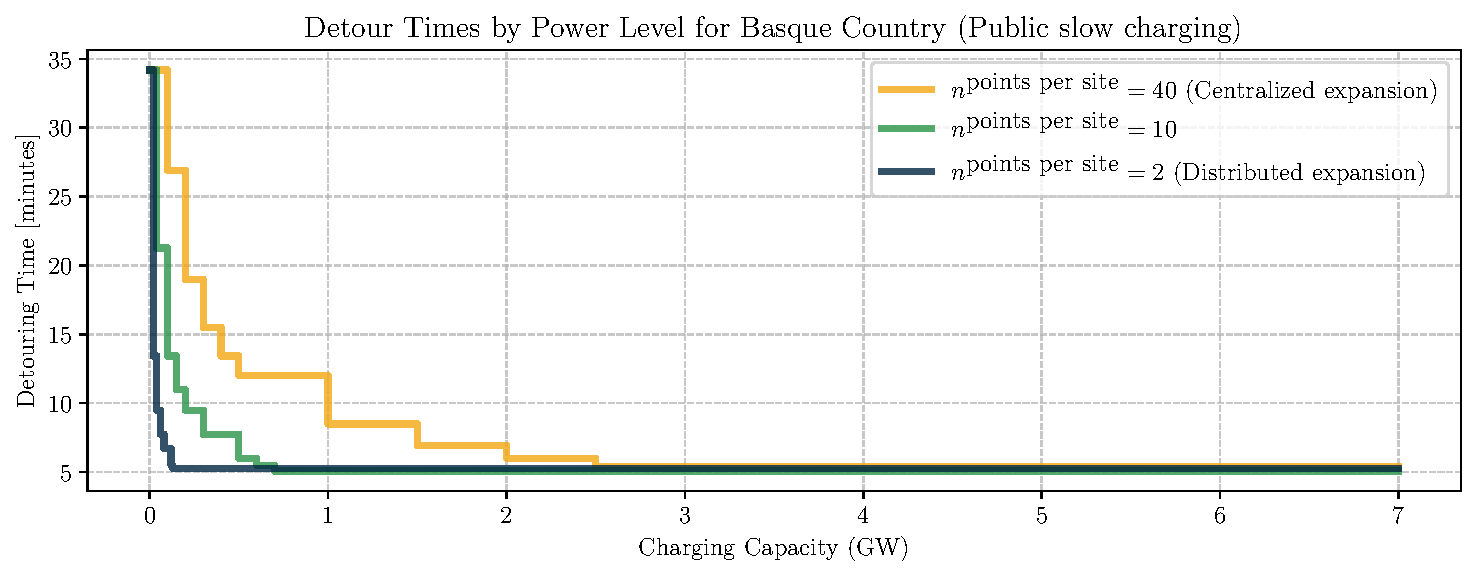
\includegraphics[width=\textwidth]{graphics/detour_time_reduction_by_capacity_and_strategy_slow.pdf}
                    
                    \vspace{1em} % optional vertical spacing
                    
                    % Bottom figure
                    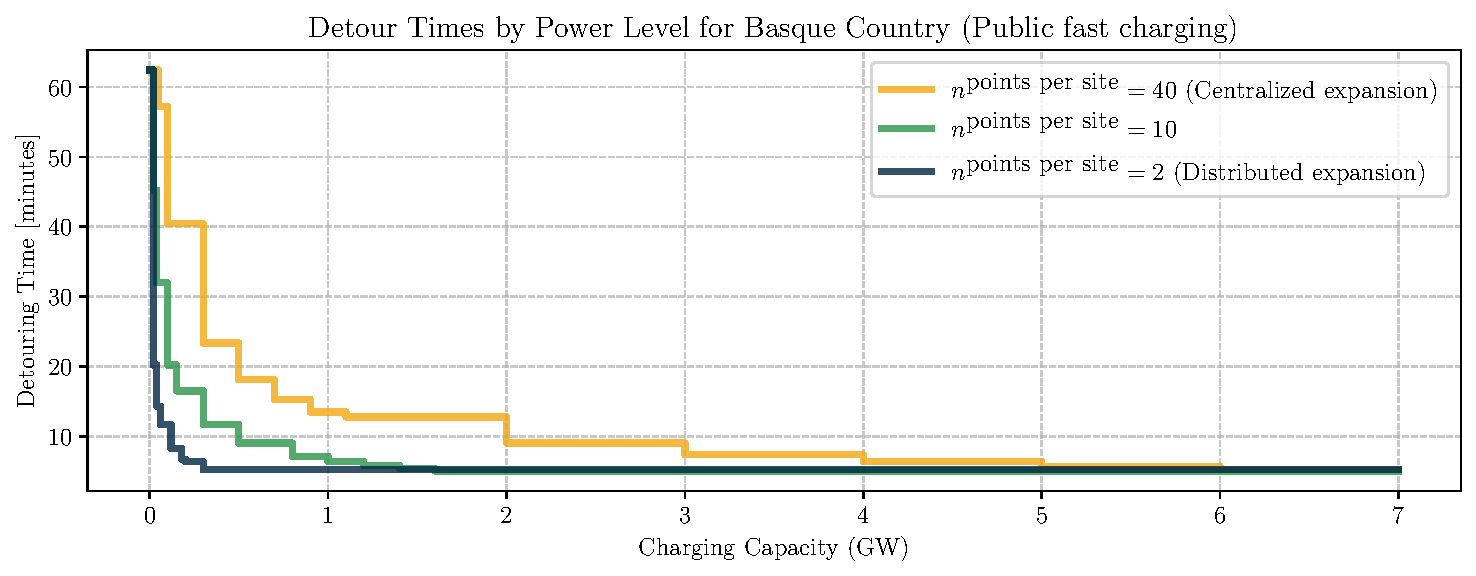
\includegraphics[width=\textwidth]{graphics/detour_time_reduction_by_capacity_and_strategy_fast.pdf}
                    
                    % One caption for both
                    \caption{Comparison of two vertically aligned figures.}
                    \label{fig:reduction}
                \end{figure}
        \subsubsection{Speed of roll-out (RQ2).}  \label{sec:rq2_scendesign}
        
        The setup for the analysis of RQ2 is displayed in the bottom row of Figure \ref{fig: scenario_design}: We consider \deleted{the }BEV adoptions in the three NUTS-3 level regions of the Basque Country and focus on the accelerated charging infrastructure expansion in Bizkaia, while observing the neighboring regions, Araba and Gipuzkoa. For this analysis, we assume the charging infrastructure capacities exogenously by including hard constraints for the infrastructure capacities. Table \ref{tab:expansion_speed} displays an overview of the designed scenarios for the analysis. \textit{Baseline Roll-out} defines a reference scenario based on the disaggregated expansion pathway to the region. The \textit{Central Acc. Roll-out} is designed to analyse the relative changes in \deleted{the }electrification\added{ compared} to this reference scenario caused by an increase of charging infrastructure by 30\%. In the scenarios \textit{Neighbor Slower Roll-out} and \textit{Central Acc. + Neighbor Slowed Roll-out}, the neighboring regions have slower expansion than the reference, and the charging capacity roll-out pathway is reduced by \deleted{-}$30\%$. These two scenarios differ again by first assuming the reference expansion pathway and in the second, the accelerated expansion with a charging capacity increased by $30\%$ to the reference. 
        \begin{table}[H]
\centering
\caption{Scenarios for analysing RQ2. The cross indicates the assumed expansion pathway for the regions in each scenario.}
\label{tab:expansion_speed}
\begin{tabular}{llccc}
\hline
                                                         &                      & \multicolumn{3}{c}{\textit{\textbf{Expansion pathway}}} \\ \cline{3-5} 
\textbf{Scenario name (RQ2)}                             & \textbf{Region name} & -30\%            & Reference         & +30\%            \\ \hline
\multirow{3}{*}{Baseline Roll-out}                       & Bizkaia              &                  & $\times$          &                  \\             
                                                         & Gipuzkoa             &                  & $\times$          &                  \\
                                                         & Araba                &                  & $\times$          &                \\ \hline
\multirow{3}{*}{Central Acc. Roll-out}                   & Bizkaia              &                  &                   & $\times$         \\ 
                                                         & Gipuzkoa             &                  & $\times$          &                  \\
                                                         & Araba                &                  & $\times$          &                  \\ \hline
\multirow{3}{*}{Neighbor Slowed Roll-out}                & Bizkaia                &          &  $\times$                  &                  \\
                                                         & Gipuzkoa             & $\times$         &                   &                  \\
                                                         & Araba              & $\times$                 &          &                  \\ \hline
\multirow{3}{*}{Central Acc. + Neighbor Slowed Roll-out} & Bizkaia                 &         &                   &    $\times$              \\
                                                         & Gipuzkoa             & $\times$         &                   &                  \\
                                                         & Araba             & $\times$                  &                   &          \\ \hline
\end{tabular}
\end{table}
    The reference expansion pathway is determined based on a model run, during which the constraint of 100\% decarbonized passenger car fleet is imposed. The resulting total charging capacity values for the investment periods between 2020 and 2050 are included as hard constraints for the charging capacity expansion. Figure \ref{fig:ref_cap} displays the reference values by region. 

        \begin{figure}[H] 
            \centering
                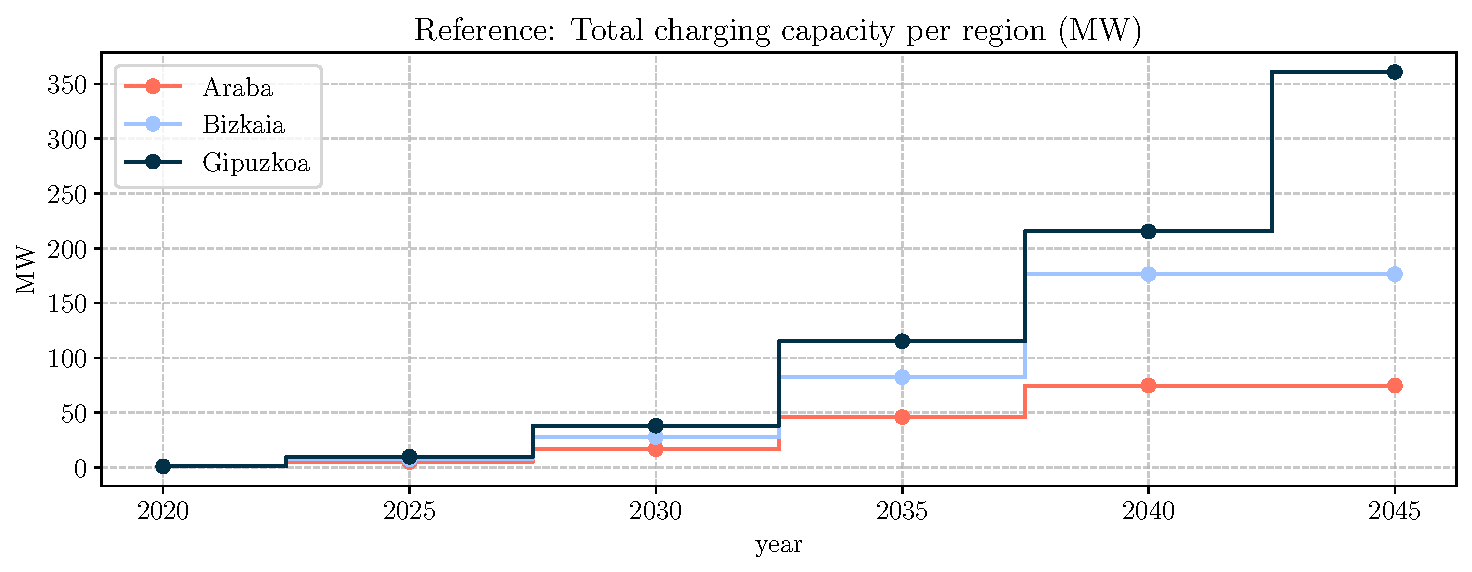
\includegraphics[width=\textwidth]{graphics/charging_capacity_per_region.pdf}
                \caption{Reference expansion pathway for scenario design of different charging capacity build-up scenarios.}\label{fig:ref_cap}
        \end{figure}
       

        % Please add the following required packages to your document preamble:

\subsection{Computational Details and data availability}
    The simulations are performed using AMD Ryzen Threadripper 7980X 64-Cores (64 cores, 3.20 base clock and 5.2 GHz boost)and 512GB RAM storage. Julia package JuMP 1.9 \citep{Lubin2023} and Gurobi 12.0\citep{gurobi} are used for the model implementation and solution. \replaced{The scripts for data preprocessing and modeling will be made available upon request}{The model and data is available in the following repository: \url{https://github.com/antoniamgolab/iDesignRES_transcompmodel}}.

\newpage
                
            
            
                

\section{Results} \label{sec:res}
    In this section, we present the most relevant results that directly address the two research questions of this work. First, we analyze the different scenarios of the spatial densification in the rollout of the public charging infrastructure network. This analysis is conducted for the Basque Country at the NUTS-2 level. Second, we zoom in on the NUTS-3 region level and examine the impact of accelerated charging infrastructure expansion in Bizkaia on the neighboring regions, Araba and Gipuzkoa. 

    
    % Please add the following required packages to your document preamble:
    % \usepackage{booktabs}
    \subsection{Income-class dependent impact of spatial densification of public charging infrastructure} \label{sec:res_1_ic}
        Figure \ref{res_1} displays two snapshots of the development of the share of electrification in the passenger car fleet by consumer group: years 2030 and 2040. $n^{\textrm{points per site}}$ indicates how many charging points are installed in newly built charging stations as of 2020, implying the degree of spatial densification of the public charging infrastructure network. The development of\deleted{ the} technology turnover is different among the consumer groups. In 2030, the electrification in the vehicle fleet belonging to the \textit{Very high income} and \textit{High income} consumer group\added{s} is significantly higher, at the level of around 48.9-65.1\%, than that of the vehicle fleet belonging to the other consumer groups. By 2040, the share of BEVs rises in all consumer groups to the level of 9.6-69.0\%. It is important to note here that in absolute numbers, the BEVs in the fleet owned by the consumer group \textit{High income} do not exceed the \textit{Very high income} consumer group.
            
        \label{sec:res_1}
        \begin{figure}[H] 
                \centering
                    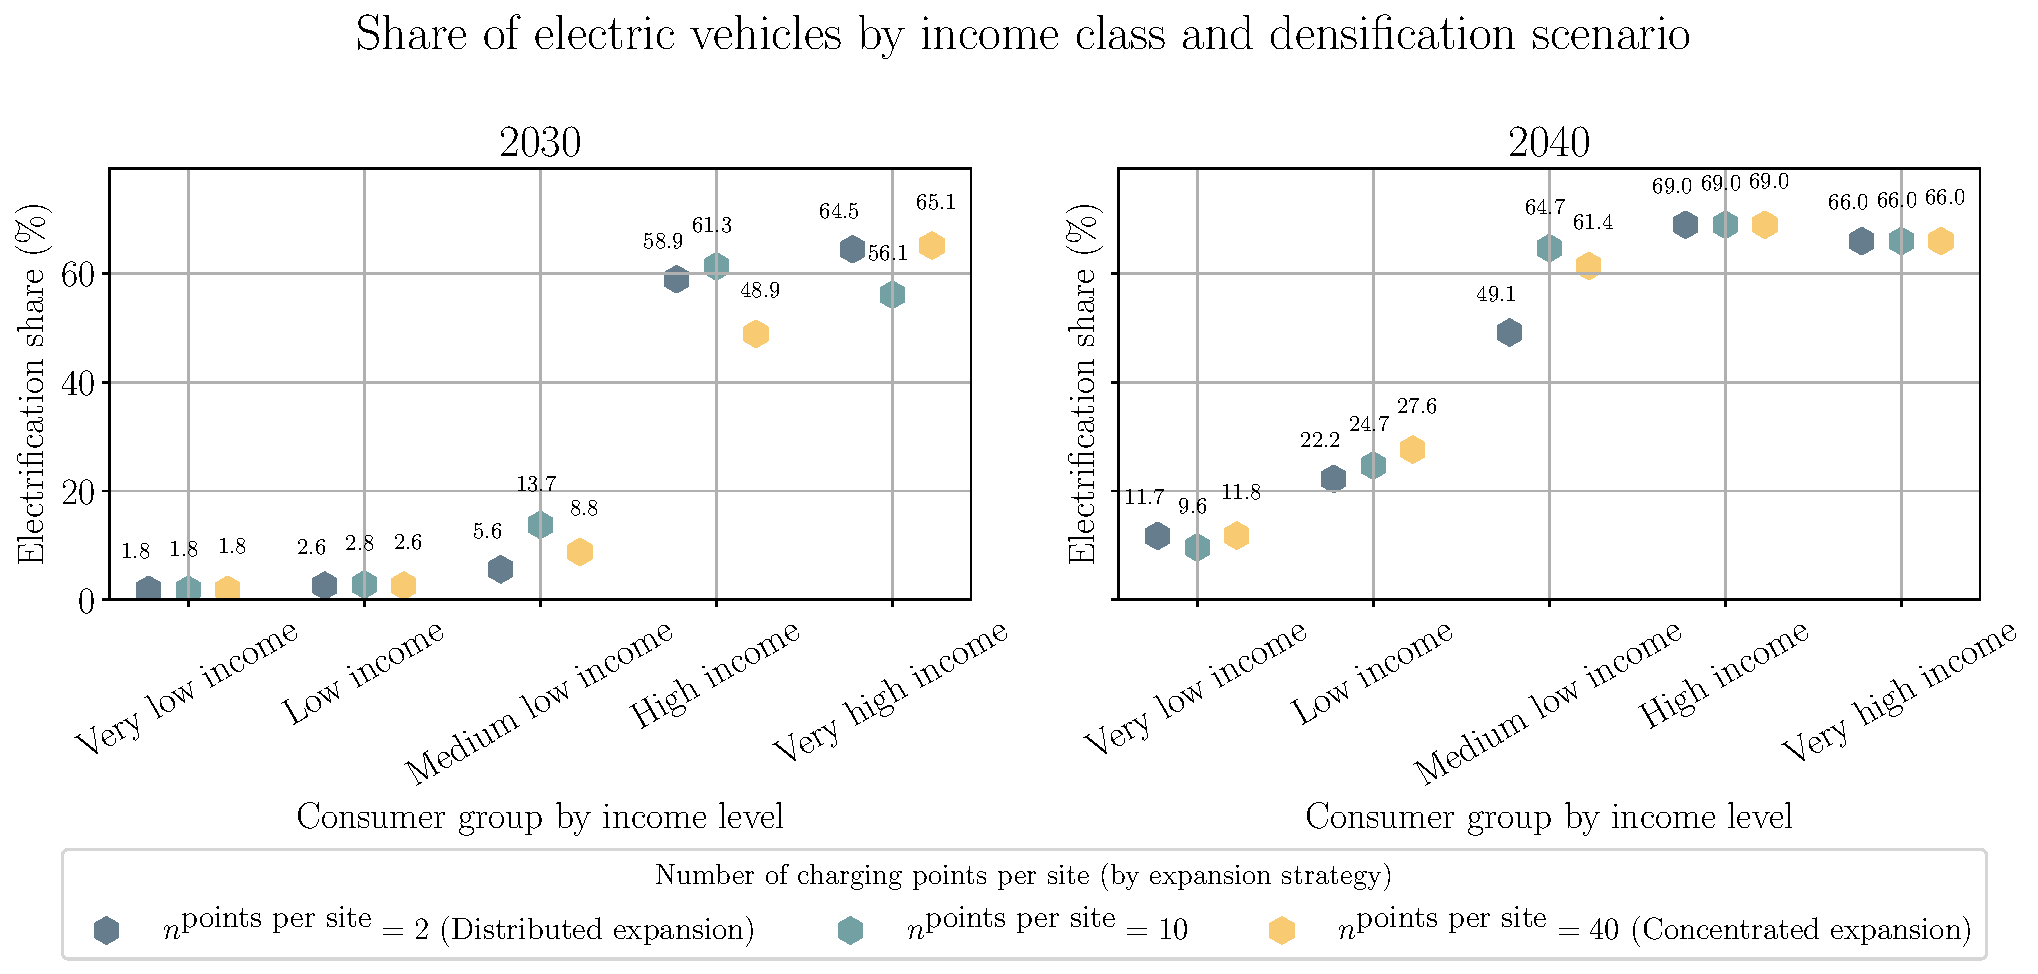
\includegraphics[width=\textwidth]{graphics/rq_1_share_electric_vehicles_by_income_and_strategy.pdf}
                    \caption{Share of battery-electric vehicles in the passenger car fleet in 2030 and 2040 in consumer groups of different income levels for roll-out strategies of public charging infrastructure defined via the number of charging points per site ($n^{\textrm{points per site}}$).}\label{res_1}
            \end{figure}
        The relative order \replaced{of}{in} the number of BEVs in the fleet by \deleted{the }consumer groups is not changed by the different roll-out strategies. \replaced{However,}{Though} significant differences in the adoption are visible between the different densification strategies: While the \textit{Concentrated expansion} leads to a gap of 6.2\% between the electrification share of the \textit{Very high income} consumer group and the \textit{High income} consumer group, this gap is lower in the scenario \textit{Distributed expansion}. The electrification of the \textit{Medium low income} group is accelerated in the more balanced scenario of ten points per site. Income groups \textit{Very low income} and \textit{Low income} are not significantly affected by 2030. By 2040, a significant gap of 5.4\% between the \textit{Distributed} and \textit{Concentrated} expansion scenario arises. 
        Overall, there is no visible correlation to be deduced between the number of points per site and the development of the electrification share in the fleets owned by the consumer groups of different income levels. 
        Figure \ref{res_add} displays differences in the development of the gap in the share of electrification between the \textit{Distributed} and \textit{Concentrated} scenarios. It shows that the highest overall impacts are on \textit{High income} and \textit{Medium low income}. By the end of the horizon, differences converge towards 0.0\%, indicating that the $n^{\textrm{points per site}}$ parameter affects the speed of electrification but is not decisive for the resulting size of \added{the }decarbonized passenger car fleet.
        
        \begin{figure}[H] 
            \centering
                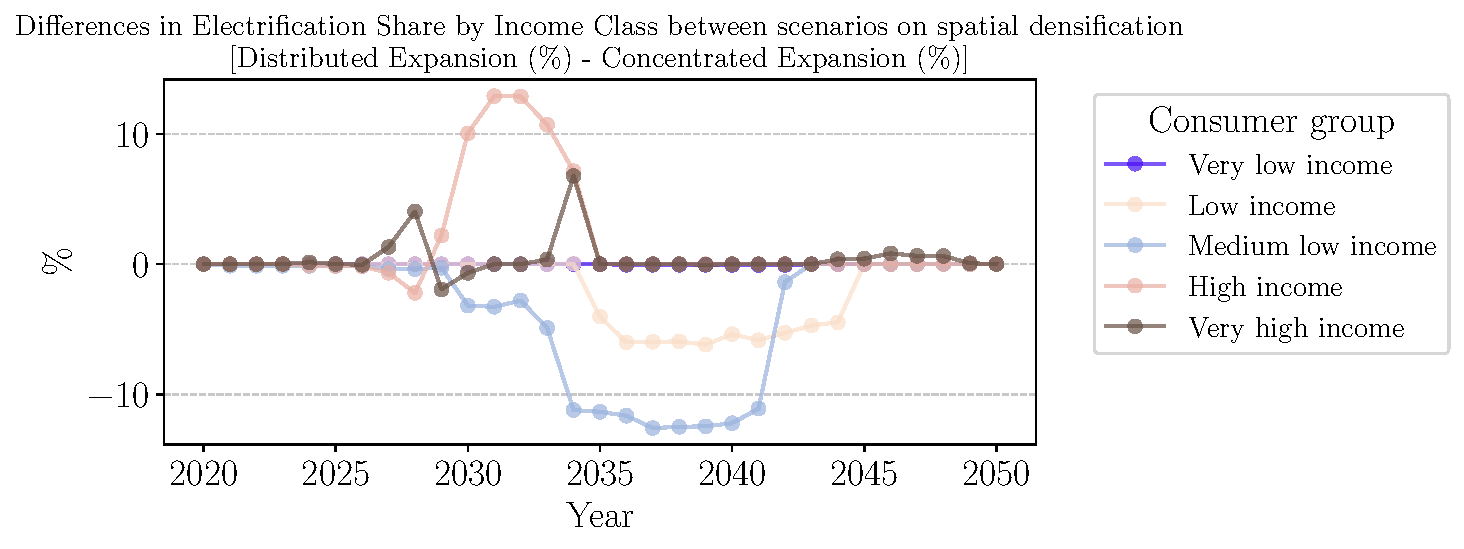
\includegraphics[width=\textwidth]{graphics/rq1_max_diff_electrification_share_by_income_class.pdf}
                \caption{Maximum differences in the electrification share between scenario $n^{\textrm{points per site}} = 2$ \textit{(Distributed expansion)} and $n^{\textrm{points per site}} = 40$ \textit{(Concentrated expansion)} by consumer groups over time.}\label{res_add}
        \end{figure}
    

        To gain a better understanding of the variation in the electrification across consumer groups, we take a look at the three key output parameters that describe the charging infrastructure expansion decisions and their utilization by scenario. Figure \ref{fig:installed_capacity} displays expanded charging infrastructure capacities together with the development of the utilization rates of public infrastructure for all scenarios. 
        Figure \ref{fig:detour_time_reduction} shows how the average detour\deleted{ing} time of public charging infrastructure is reduced by these capacity expansions. Figure \ref{res_2} illustrates the charger utilization by income class, \replaced{showing}{by} how much energy is charged by charger type and income class in years 2030, 2040, and 2050.
        
        The following observations are the most relevant here:
        \begin{itemize}
            \item With an increase of the value for the parameter $n^{\textrm{points per site}}$, higher investments in public charging infrastructure are made earlier. In the scenario $n^{\textrm{points per site}} = 10$, public charging infrastructure capacity expands more rapidly in the investment periods 2030-2040 compared to the scenario $n^{\textrm{points per site}} = 2$ (\textit{Distributed expansion}). In the scenario $n^{\textrm{points per site}} = 40$ (\textit{Concentrated expansion}), the capacity of the public charging network in 2035 equals that of the 2040 level under lower values of the $n^{\textrm{points per site}}$ parameter (see Figure \ref{fig:installed_capacity}). In scenario $n^{\textrm{points per site}} = 2$ (\textit{Distributed expansion}), substantial increases in the public charging infrastructure network \replaced{occur}{are} during later years, 2040 and 2045. In all scenarios, these investment periods of substantial expansion coincide with decreases in detouring times for public charging infrastructure (see Figure \ref{fig:detour_time_reduction}). 
            \item The accelerated expansion in the scenario $n^{\textrm{points per site}} = 10$, the increased scenarios in 2030 coincide with the sharp increase in adoption in the consumer group \textit{Medium low income} (as displayed in Figure \ref{res_1}), indicating that the increased charging capacities particularly accelerate the electrification of the passenger car fleet owned by consumer\added{s} of medium level income.
            \item Home and work charging capacities are consistent across all scenarios. While work charging is \deleted{early on }expanded\added{ early on} to its maximum possible capacity values, home charging capacities are not further expanded, though\added{ they are} used consistently by the consumer groups \textit{Very high income} and \textit{High income} as shown in Figure \ref{res_2}. 
            \item The utilization rates of public charging infrastructure diverge substantially between the slow and fast charging types. For both charger types, maximum utilization  --- indicated by the red dashed line in graphs of the right column in Figure \ref{fig:installed_capacity} --- is not reached. In particular, the utilization rate of fast charging is very low (maxima are at 6-11\%), indicating substantial investments in overcapacities.
            \item While, in all scenarios, the absolute numbers of BEVs and total energy consumption are similar by 2050, installed charging capacities and their utilization by income groups are different. Looking at the right column in Figure \ref{res_2}, there is a significant difference between the charged energy by income class and type between the scenario of $n^{\textrm{points per site}} = 2$ and the other two with charging sites of higher concentration. Particularly, there is a significant difference in the usage of fast charging by the consumer groups \textit{Very low income} and \textit{Low income}\footnote{\added{We want to emphasize here for the interpretation of the results that we do not consider the different \textit{pricing} of charging types here.}}. In the \textit{Distributed expansion} scenario, higher amounts of public charging are available and used, while, in the \textit{Very \replaced{l}{L}ow income} group, fast charging is the dominating charging technology, leading to higher total utilization of fast charging. 
            
        \end{itemize}
        \begin{figure}[H]
                \centering 
                    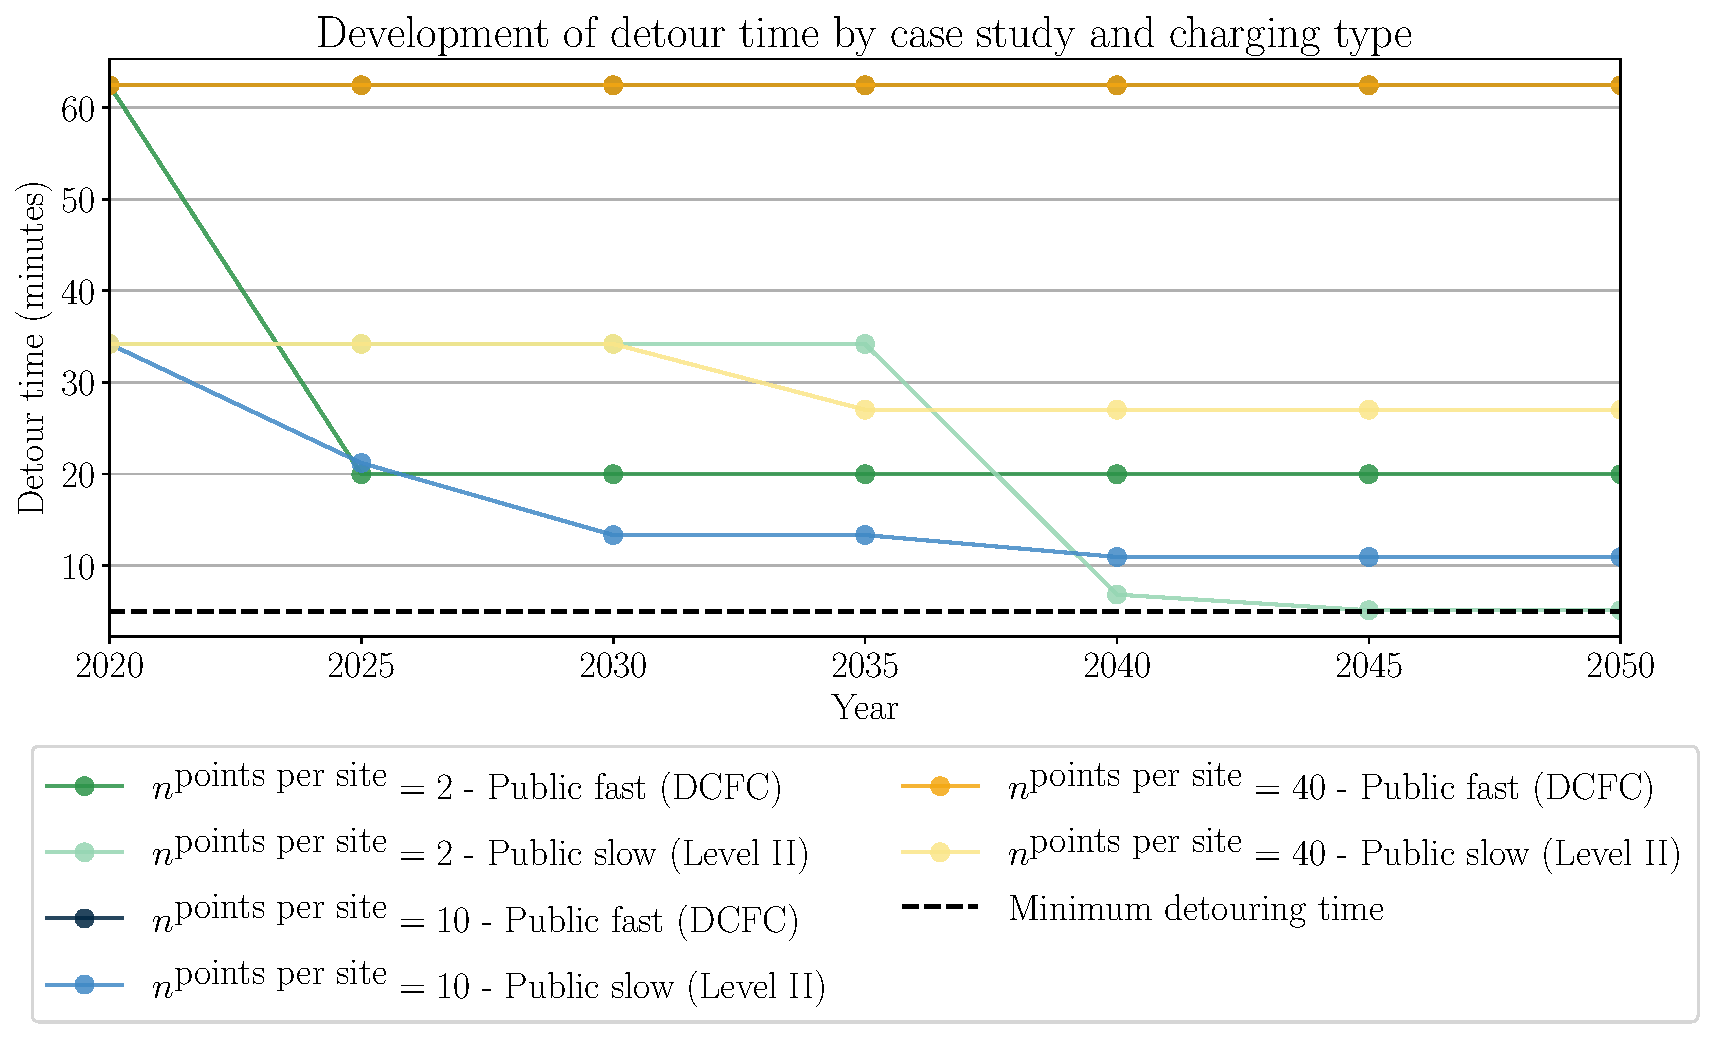
\includegraphics[width=12cm]{graphics/rq_1_detour_time_development_by_case_and_type.pdf}
                    \caption{Development of average detouring times for public fast and slow charging in Basque Country for different scenarios of spatial densification.} \label{fig:detour_time_reduction}
            \end{figure}
  
        
        % \begin{itemize}
        %     \item Interplay between detour time reduc and expansion
        %     \item leading to overcap for the sake of reducing it
        %     \item work charging being also convenient, is very attractive for very high income class 
        %     \item utilization factors fast charging, only later increase significantly 
        %     \item no home charging expanded but used by Very high and High income groups extensively 
        %     \item relation to 2030 --- simultaneous with accel. medium and high income 
        %     \item Fast charging only used by low income 
        %     \item 
        %     \item by 2050: how are utilizations different when the electrification shares are the same; dispite the 
        %     \item 

        %     \item diff n points per site parameter led to different investment decisions and charging infrastructure utilization by income class
        %     \item consistent: work charging to the max and home charging not expanded 
        %     \item in npoints = 10 - detour time is decreased the quickest, leading to accelerated electrification; 
        %     \item by 2050: same elctricification rate but different utilouzation; 2050 distributed: has lowest detouring time for slow charging; more utilization here of public charging 
        %     \item Fast charging capacities used to cover low income class level charging demand
        %     \item wenn public slow charging dense - 2035 -2040; dropped work charging 
        %     \item zwischen 2035 - 2040 - adoption verly low - medium income level -- nutzen public charging ( geringeres value of time) korreliert mit high investments in distributed (reduction) +expansion 


        % \end{itemize}        
        

        % By 2030, the \textit{Distributed expansion} accelerates the electrification of the passenger car fleet owned by the \textit{Very high income} consumer group by around 7\% compared to the centralized approach. In contrast to this stand the slightly accelerating impact of the centralized distribution to the electrification of BEVs of the \textit{High income} consumer group. In the other consumer groups, the values are not significantly impacted.  
     

    
    % Figure \ref{res_add} displays the differences between the \textit{Distributed expansion} ($n^{\textrm{points per site}} = 2$) and \textit{Concentrated expansion} ($n^{\textrm{points per site}} = 40$) scenario of the passenger car fleet of the different cases by consumer group over time. The previously described impact on consumer groups \textit{High income} and \textit{Very high income} is observed during the time frame 2020 $-$ 2037. After this, the differences between the value are close to zero. 
    
    % Figure \ref{res_2} illustrates the allocation of annually accumulated amounts of charged energy by type of charging infrastructure for years 2030 and 2040. The results of scenario  $n^{\textrm{points per site}} = 2$ is here contrasted with the more concentrated densification roll-out scenarios of $n^{\textrm{points per site}} = 10$ and $n^{\textrm{points per site}} = 40$. In 2030, in the \textit{Distributed expansion}scenario, most charging processes are allocated at public slow charging infrastructure, while, in the other two scenarios, public slow charging plays a secondary role. By 2040, in the \textit{Distributed expansion}  scenario, work charging is used throughout most of the consumer groups, while this is exclusively used by the \textit{Very high income} consumer group in the $n^{\textrm{points per site}} = 10$ scenario and by the \textit{High income} group in the $n^{\textrm{points per site}} = 40$ scenario. Throughout all scenarios, public fast charging is exclusively used by the \textit{Very low income} consumer group. This overall pattern of high utilization of public slow in comparison to public fast charging infrastructure also becomes evident in the development of utilization rates displayed over time in Figure \ref{fig:load_factors}. The values of the utilization rate do not vary significantly by scenario. Figure \ref{fig:load_factors} displays the values for the setting of $n^{\textrm{points per site}} = 10$. The wave-like pattern results from the previous definition of the five-year investment periods, which are indicated by the arrows. The red dashed line is placed at 25\%, which is the maximum possible utilization rate used for the sizing of capacity in the simulation. We observe that this limit is never reached, and more public charging capacity is installed than required. 
    
    % Figure \ref{fig:installed_capacity} displays the development of expanded charging infrastructure for $n^{\textrm{points per site}} = 40$. The charging infrastructure for work places is expanded to its maximum possible capacity early on, already by 2025, while no additional capacities are added to home charging. The red line indicates the upper bound for maximum charging infrastructure expansion that is set in the simulations. This upper limit is exhausted during early years of expansion. 
    
    % In Figure \ref{fig:detour_time_reduction}, we display the development of the reductions of the detouring time through the expansion and therefore densification of the public charging network. The 5-minute mark (black dashed line) indicates the minimum possible detour time that was used in the preperation of the data. The reductions of detouring time happen within the time frame between 2020-2040. 
    % Only in the case of distributed densification, the minimum detouring time is achieved.

    
        


        \begin{figure}[H]
        \centering 
            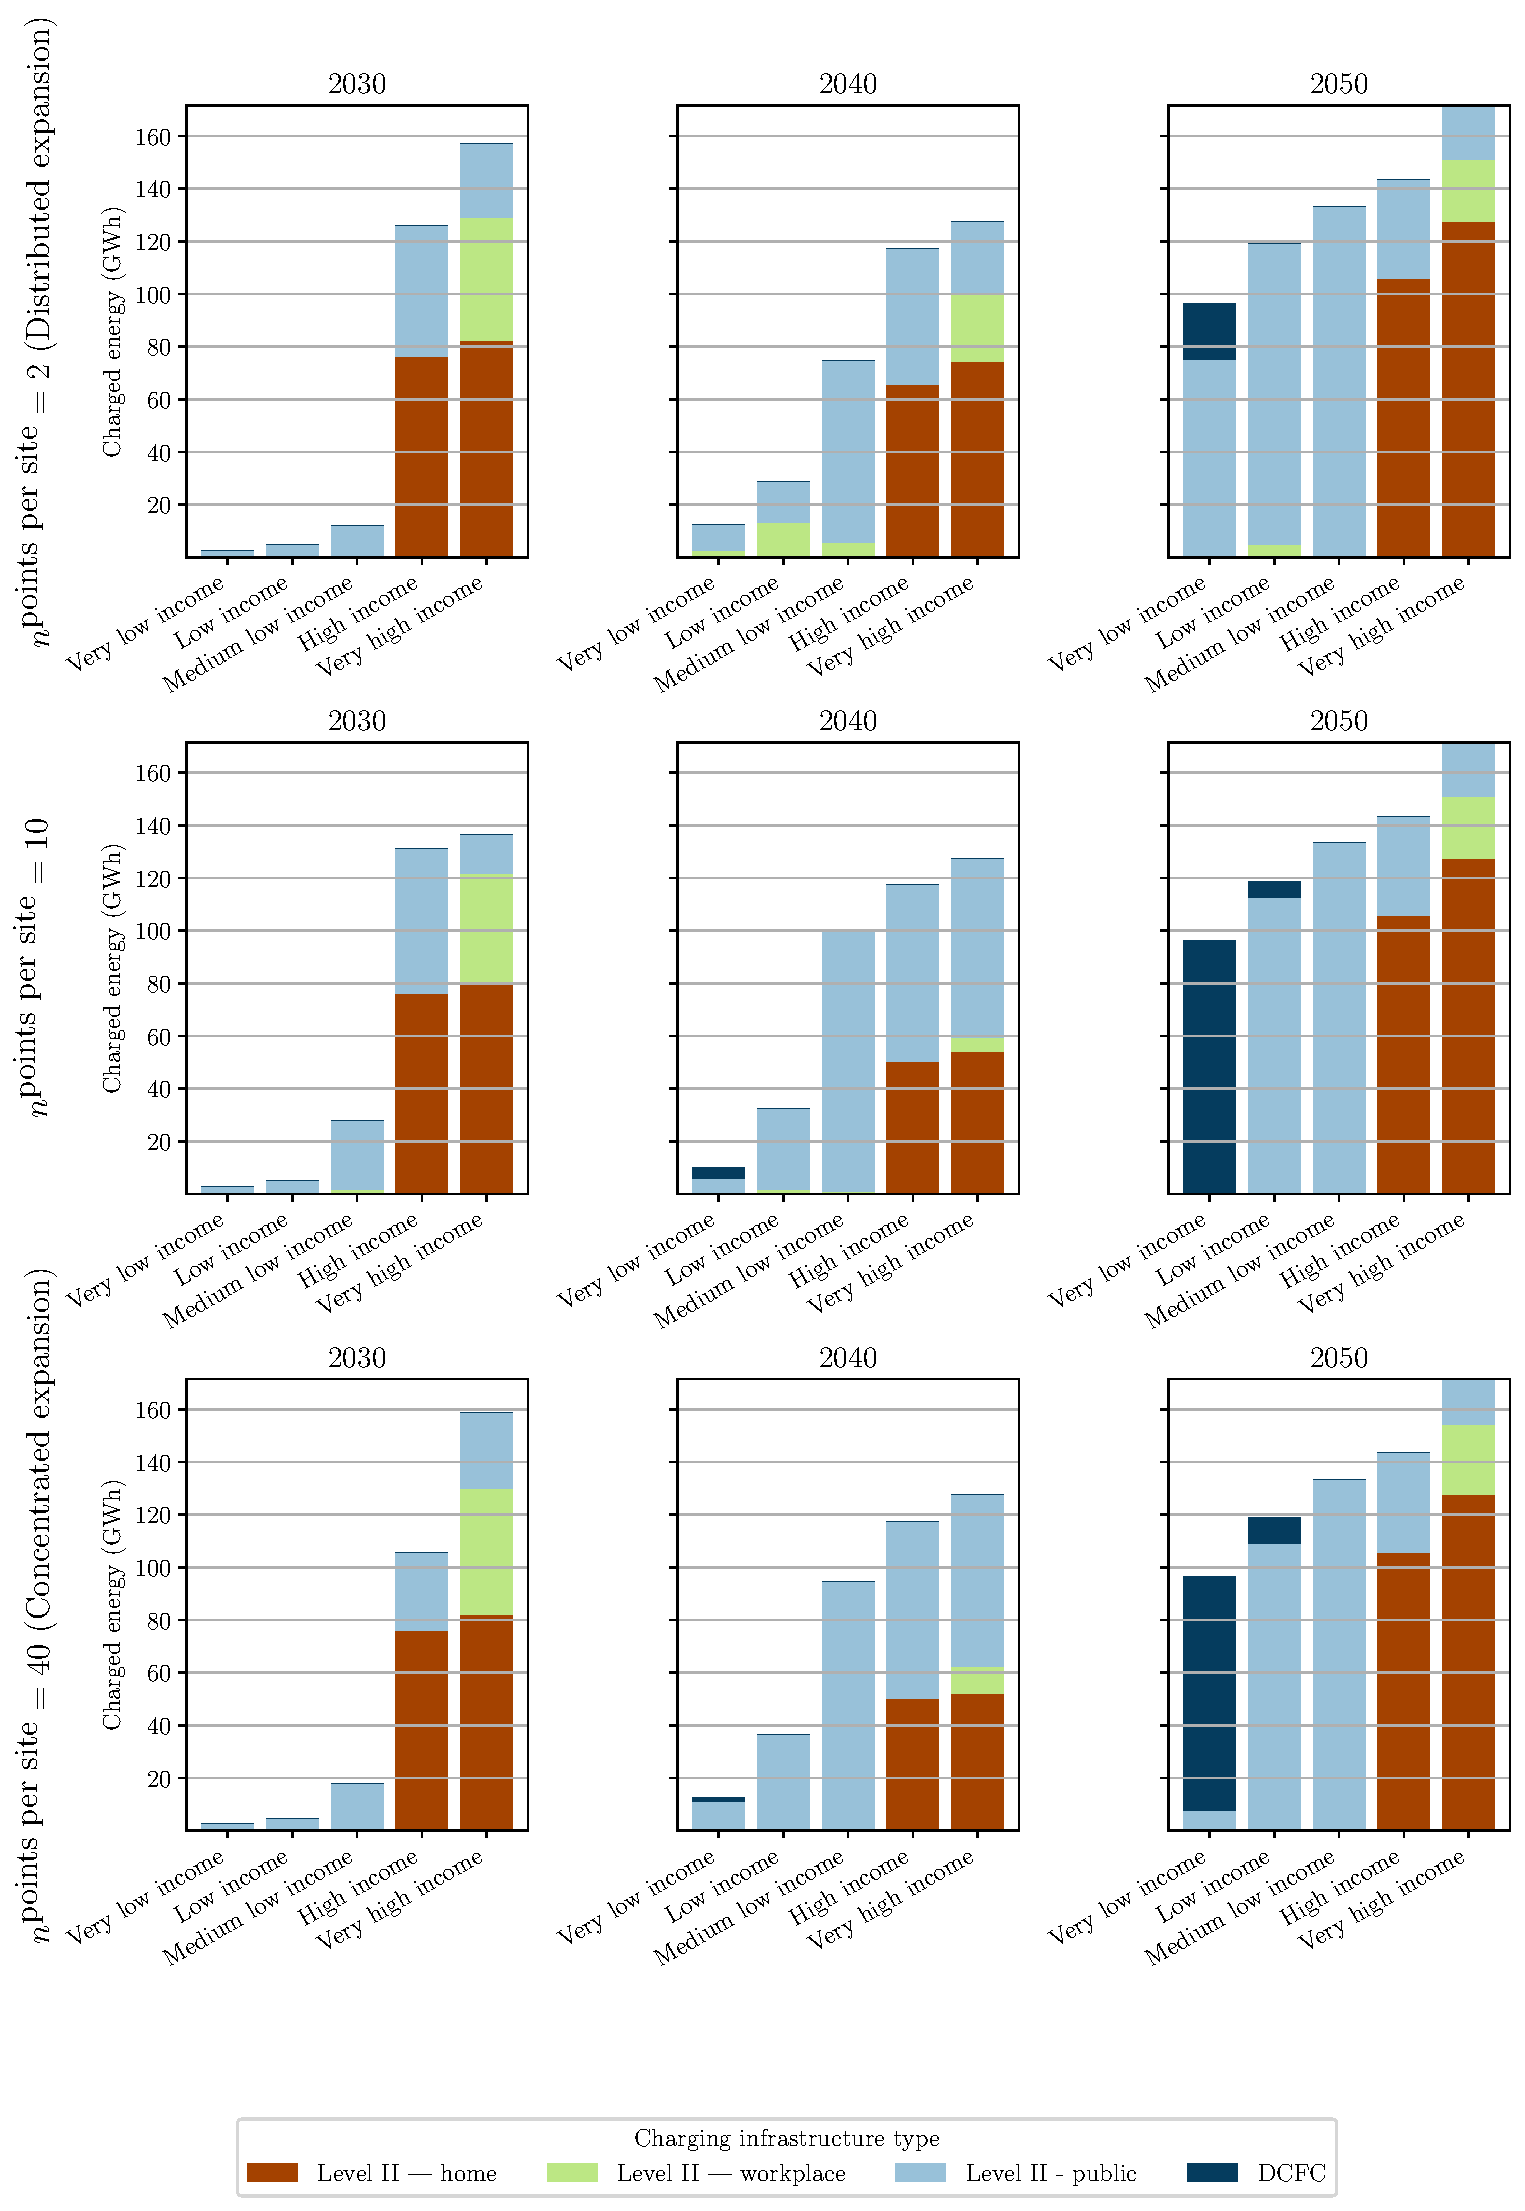
\includegraphics[width=12cm]{graphics/rq_1_fueled_energy_by_income_class_and_year_grid.pdf}
            \caption{Charged energy in 2030, 2040 and 2050 at different infrastructures}\label{res_2}
        \end{figure}
        %         \begin{figure}[H]
        %     \centering
        %         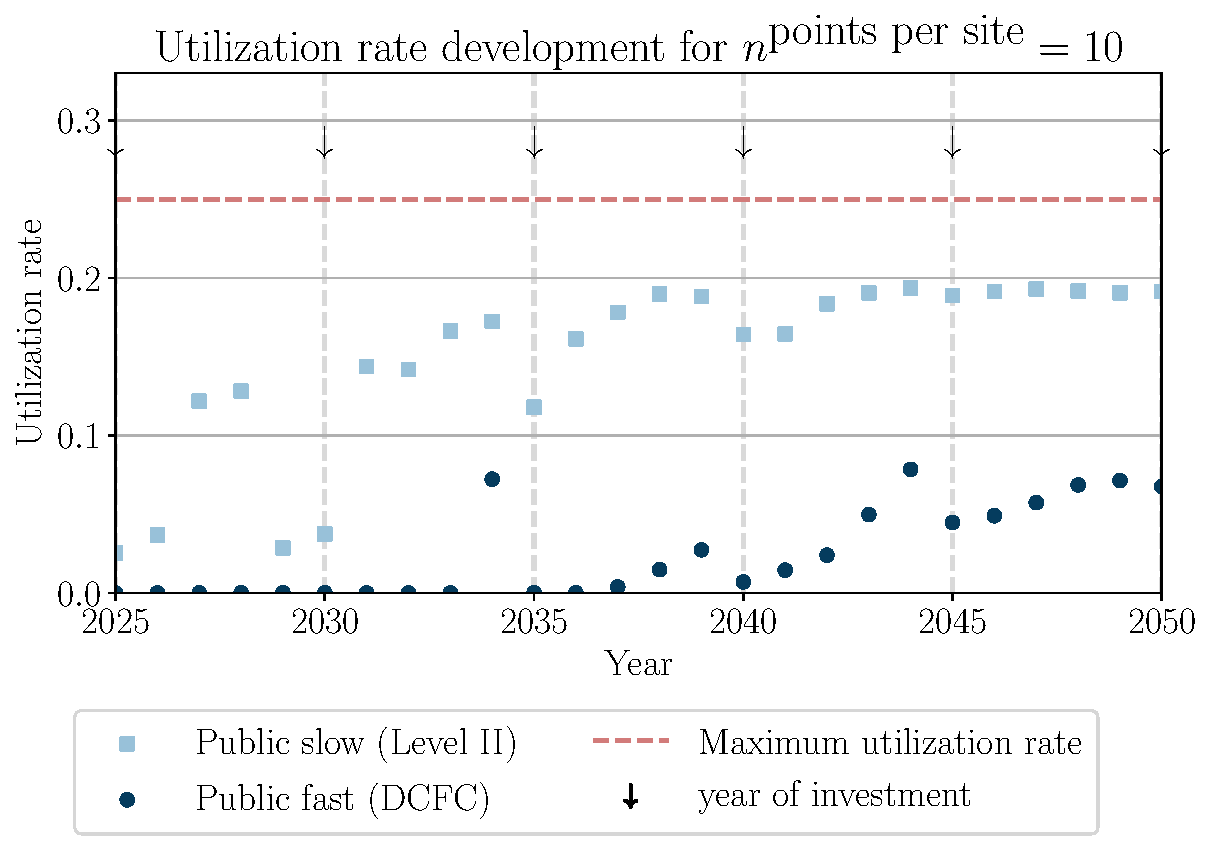
\includegraphics[width=10cm]{graphics/rq_1_load_factor_development_balanced_densification.pdf}
        %         \caption{Utilization rate of public slow and public fast infrastructure.} \label{fig:load_factors}
        % \end{figure}
        \begin{figure}[H]
            \centering
                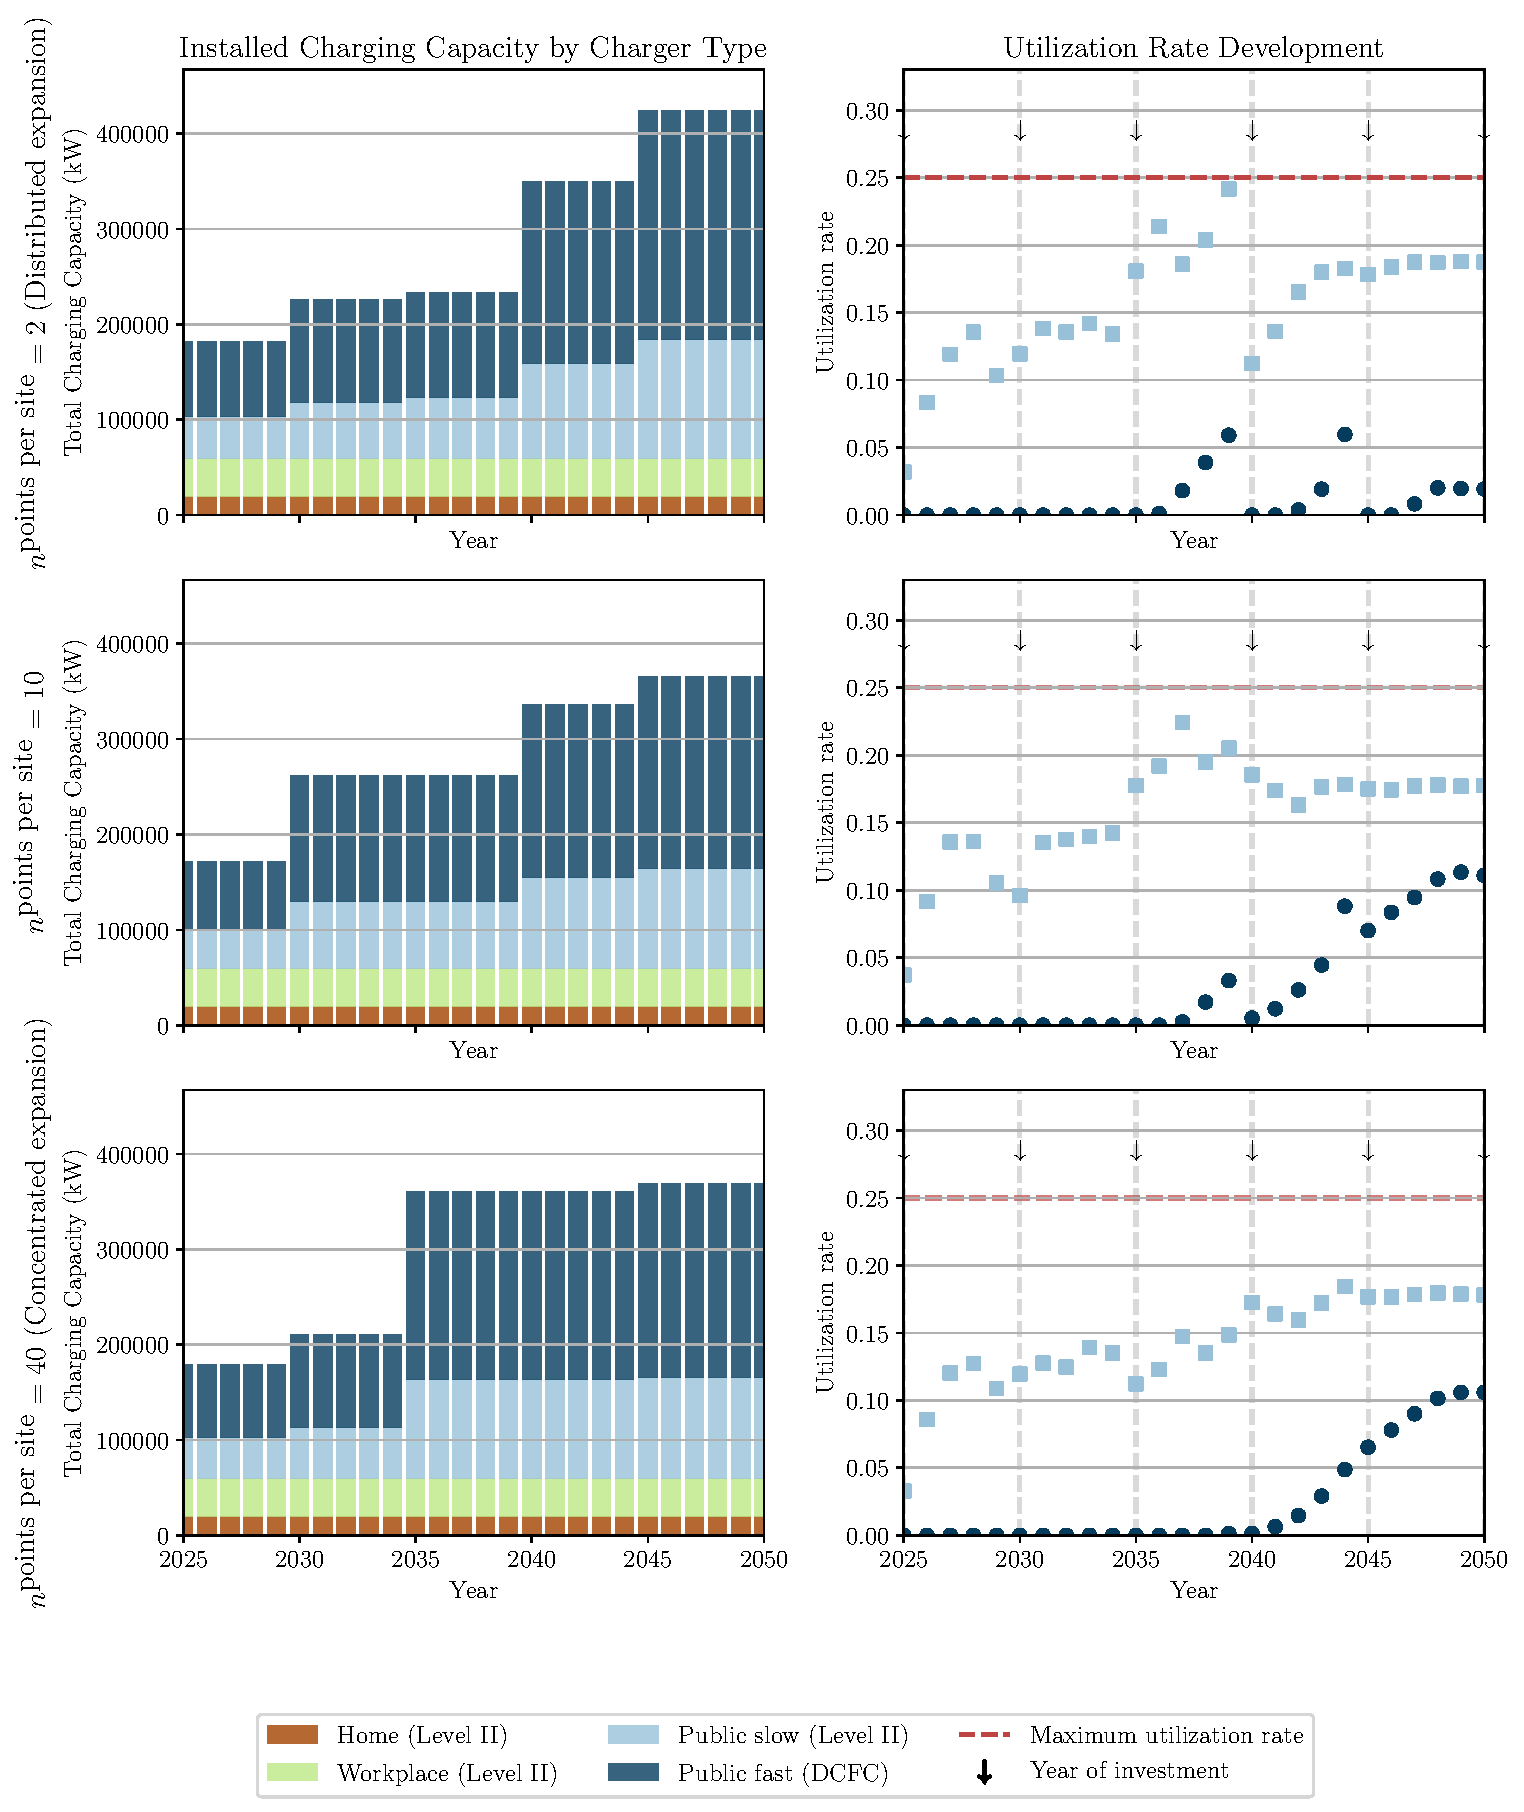
\includegraphics[width=\textwidth]{graphics/rq_1_installed_capacity_and_load_factor_centralized_densif.pdf}
                \caption{Charging infrastructure expansion for Basque Country region in the scenario of \textit{Concentrated expansion} ($n^{\textrm{points per site}} = 40$).} \label{fig:installed_capacity}
        \end{figure}




    % TODO 
    %\todo{Add analysis on the different impact on commercial segment (high budget + high value of time + long distances)}
    % \subsection{Vehicle stock turnover}

    % \subsection{Technological shift in different consumer groups }
    % \subsection{When are vehicles purchased and when not ... }
    % \begin{itemize}
    %     \item Are these dynamics changing? In terms of lifetime of passenger car vehicles? 
    % \end{itemize}
    % \subsection{\dots}
    \subsection{Spill-over effect of charging infrastructure planning for destination charging} \label{sec:res_2}

    
    Figure \ref{fig:rq2_1} displays the development of the adoption of BEVs by years 2030 and 2040. In particular, this is shown for the NUTS-3 regions Bizkaia, Araba\added{,} and Gipuzkoa, under the different scenarios in the speed of charging infrastructure expansion. In the \textit{Baseline Roll-out} case, in 2030, the range of the electrification rate varies by region within 2.6-6.0\%. By 2040, the region-dependent range becomes wider, 35.5-42.8\%, with Araba having the highest rate of electrification and Bizkaia the lowest. With increased charging capacities built in Bizkaia (case \textit{Central Acc. Roll-out}), the electrification share in Bizkaia increases slightly (0.9 \% by 2030 and 3.3\% by 2040), while the electrification rates of Araba and Gipuzkoa are also positively affected (increase by 0.6-1.3\%). When the charging infrastructure capacity in Araba and Gipuzkoa (scenarios \textit{Neig\added{h}bor Slowed Roll-out} and \textit{Central Acc. + Neig\added{h}bor Slowed Roll-out}) are reduced, the values for the share of electrification in Araba and Gipuzkoa in 2040 are significantly lower than in \textit{Baseline Roll-out}. \added{Figure \ref{fig:rq2_temp} displays the temporal development of the difference in electric vehicle numbers between the\textit{Central Acc. Roll-out} and the \textit{Baseline Roll-out}. A peak in the positive absolute differences occurs in 2045. The maximum relative difference is in 2044 and is 2.1\% for Araba and 1.1\% for Gipuzkoa. For some time periods, we observe negative spillover. In particular, there is a distinctive decrease in the BEV numbers in 2049.}
        
    \begin{figure}[H]
            \centering
                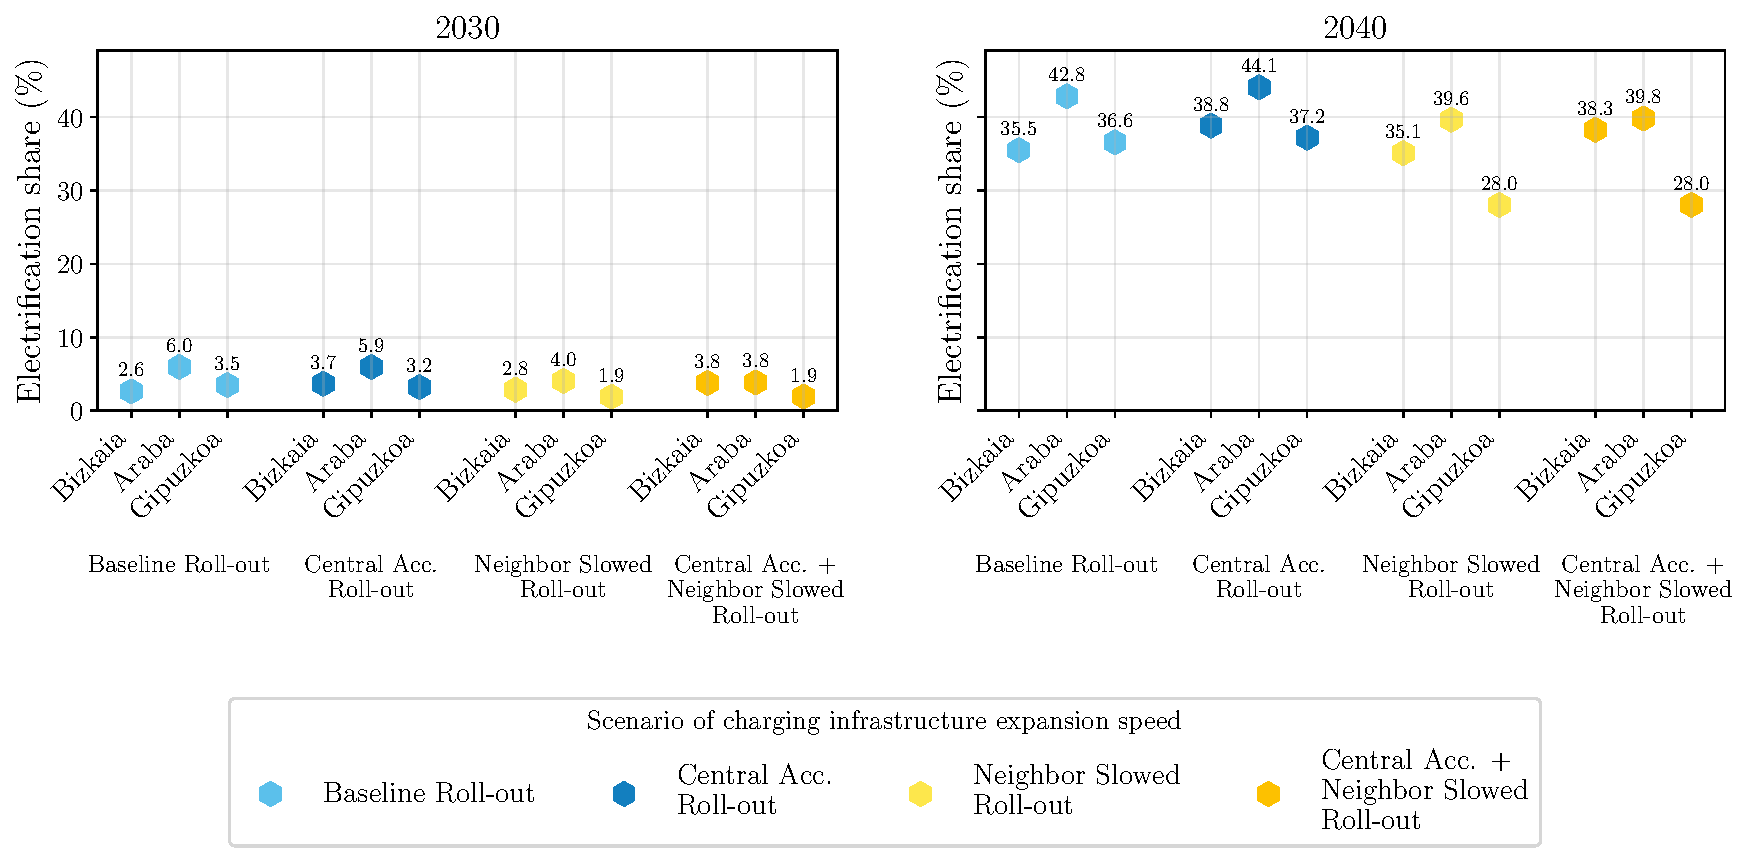
\includegraphics[width=\textwidth]{graphics/rq_2_electrification_share_by_scenario_and_region.pdf}
                \caption{Share of electrification of the passenger car fleet in the regions Bizkaia, Araba, and Gipuzkoa under different scenarios referring to the speed of charging infrastructure roll-out, for years 2030 and 2040.} \label{fig:rq2_1}
        \end{figure}
    
     \begin{figure}[H]
            \centering
                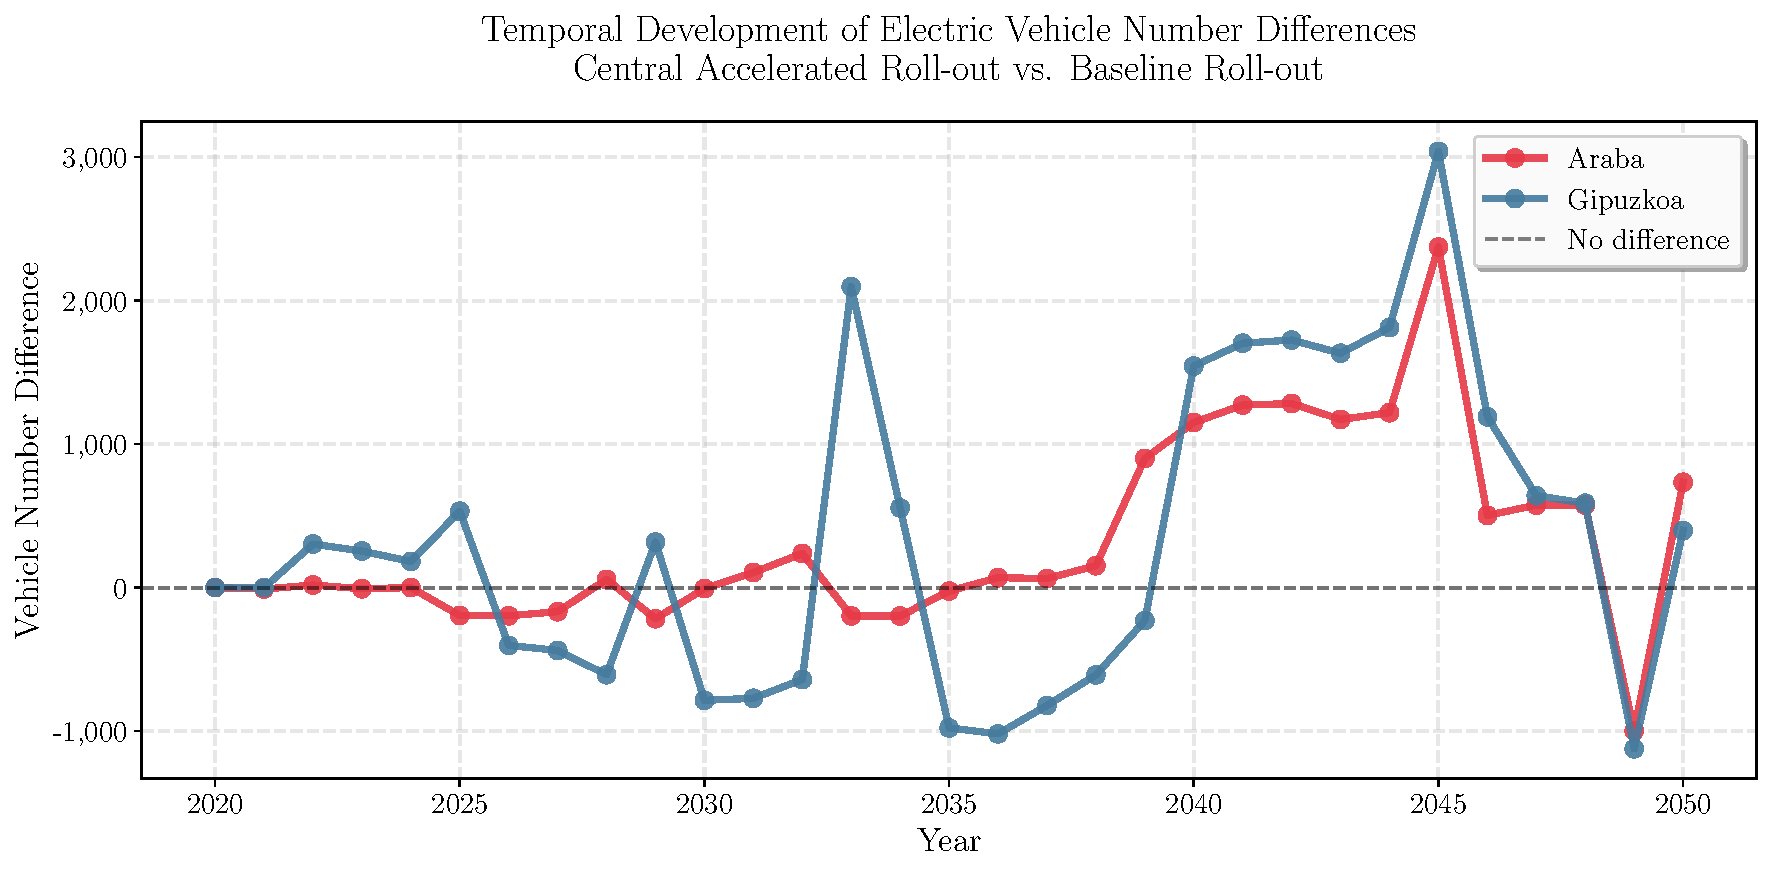
\includegraphics[width=0.8\textwidth]{graphics/rq_2_vehicle_difference_temporal_development.pdf}
                \caption{\added{Temporal development of the difference of adopted battery electric vehicles numbers in Araba and Gipuzkoa between the \textit{Basic Roll-out} and \textit{Central Acc. Roll-out.}}} \label{fig:rq2_temp}
        \end{figure}
    
    With higher expansion in Bizkaia in \textit{Central Acc. + Neighbor Slowed Roll-out}, the electrification share in Bizkaia is increased by 2.1\% by 2040. \replaced{The BEV adoption shares in Araba and Gipuzkoa}{The impact on the BEV adoption share in Araba and Gipuzkoa} are here impacted significantly less, i.e.\added{,} than in the reference capacity expansion. In 2030, a slight negative impact is observed.

    Figure \ref{fig:rq2_2} gives an insight into the effect of increased charging capacity in Bizkaia on the electrification of the commuting traffic. The plots display the absolute numbers of BEVs used for commuting trips originating in Araba or Gipuzkoa and traveling to Bizkaia. We zoom in on three years: 2030, 2040, and 2050. The text in blue indicates the relative differences to the \textit{Baseline Roll-out} scenario. The gray text indicates the relative difference to \textit{Neighbor Slowed Roll-out}. The following \replaced{four}{three} key observations are made here:
    
    \begin{itemize}

        
        \item The slowed roll-out in Araba and Gipuzkoa has little impact on the BEV adoption in the commuting fleet. Some negative impact is observed during 2040-2050 which is partly compensated with increased capacities in Bizkaia.

        \item In Araba, the electrification of the commuting fleet is mainly positively accelerated during the years 2030 and 2040 by the increased charging infrastructure deployment in Bizkaia. By 2050, this positive impact is limited to $+0.6\%$. 

        \item In Gipuzkoa, the impact of increased infrastructure expansion in Bizkaia remains not significant.

        \item In the case of reduction of charging infrastructure in Araba and Gipuzkoa, the increased charging infrastructure in Bizkaia does not fully compensate for the reduced capacities. 
            
    \end{itemize}

    %Figure \ref{fig:rq2_4} underscores these temporal differences in the effect of the increased charging capacities at the destination region. This figure displays the distribution of the relative differences between the scenarios of increased charging charging capacity and the corresponding references. The red curve indicates the average difference. The grey area is the 95\% quantile range of the curves. While there are some negative effects on the adoption rate in early years, the effect on the adoption in commuting trips is overall positive, indicating a significant acceleration of the BEV adoption. This acceleration only takes place in the years around 2025 to 2035. After this. the effects of the increased charging infrastructure decrease rapidly.  
    
    In Figure \ref{fig:rq2_3}, we examine the allocation of charging processes for commuting trips between the origin and destination regions. We generally observe a high share of destination charging across all cases, years, and both regions. These shares increase under the accelerated rollout in Bizkaia. One exception is the development in Gipuzkoa between 2030 and 2040, during which there is a 43\% increase in charging processes at the origin (between the Central Acc. Roll-out and Baseline Roll-out scenarios).

    Figure \ref{fig:rq2_5} displays utilization rates for the public charging infrastructure in the Baseline Roll-out across all three regions. Here again, utilization rates of public slow charging are consistently higher than those of public fast charging. Overall, utilization rates are significantly higher when spatial density is not considered.


         \begin{figure}[H]
            \centering
                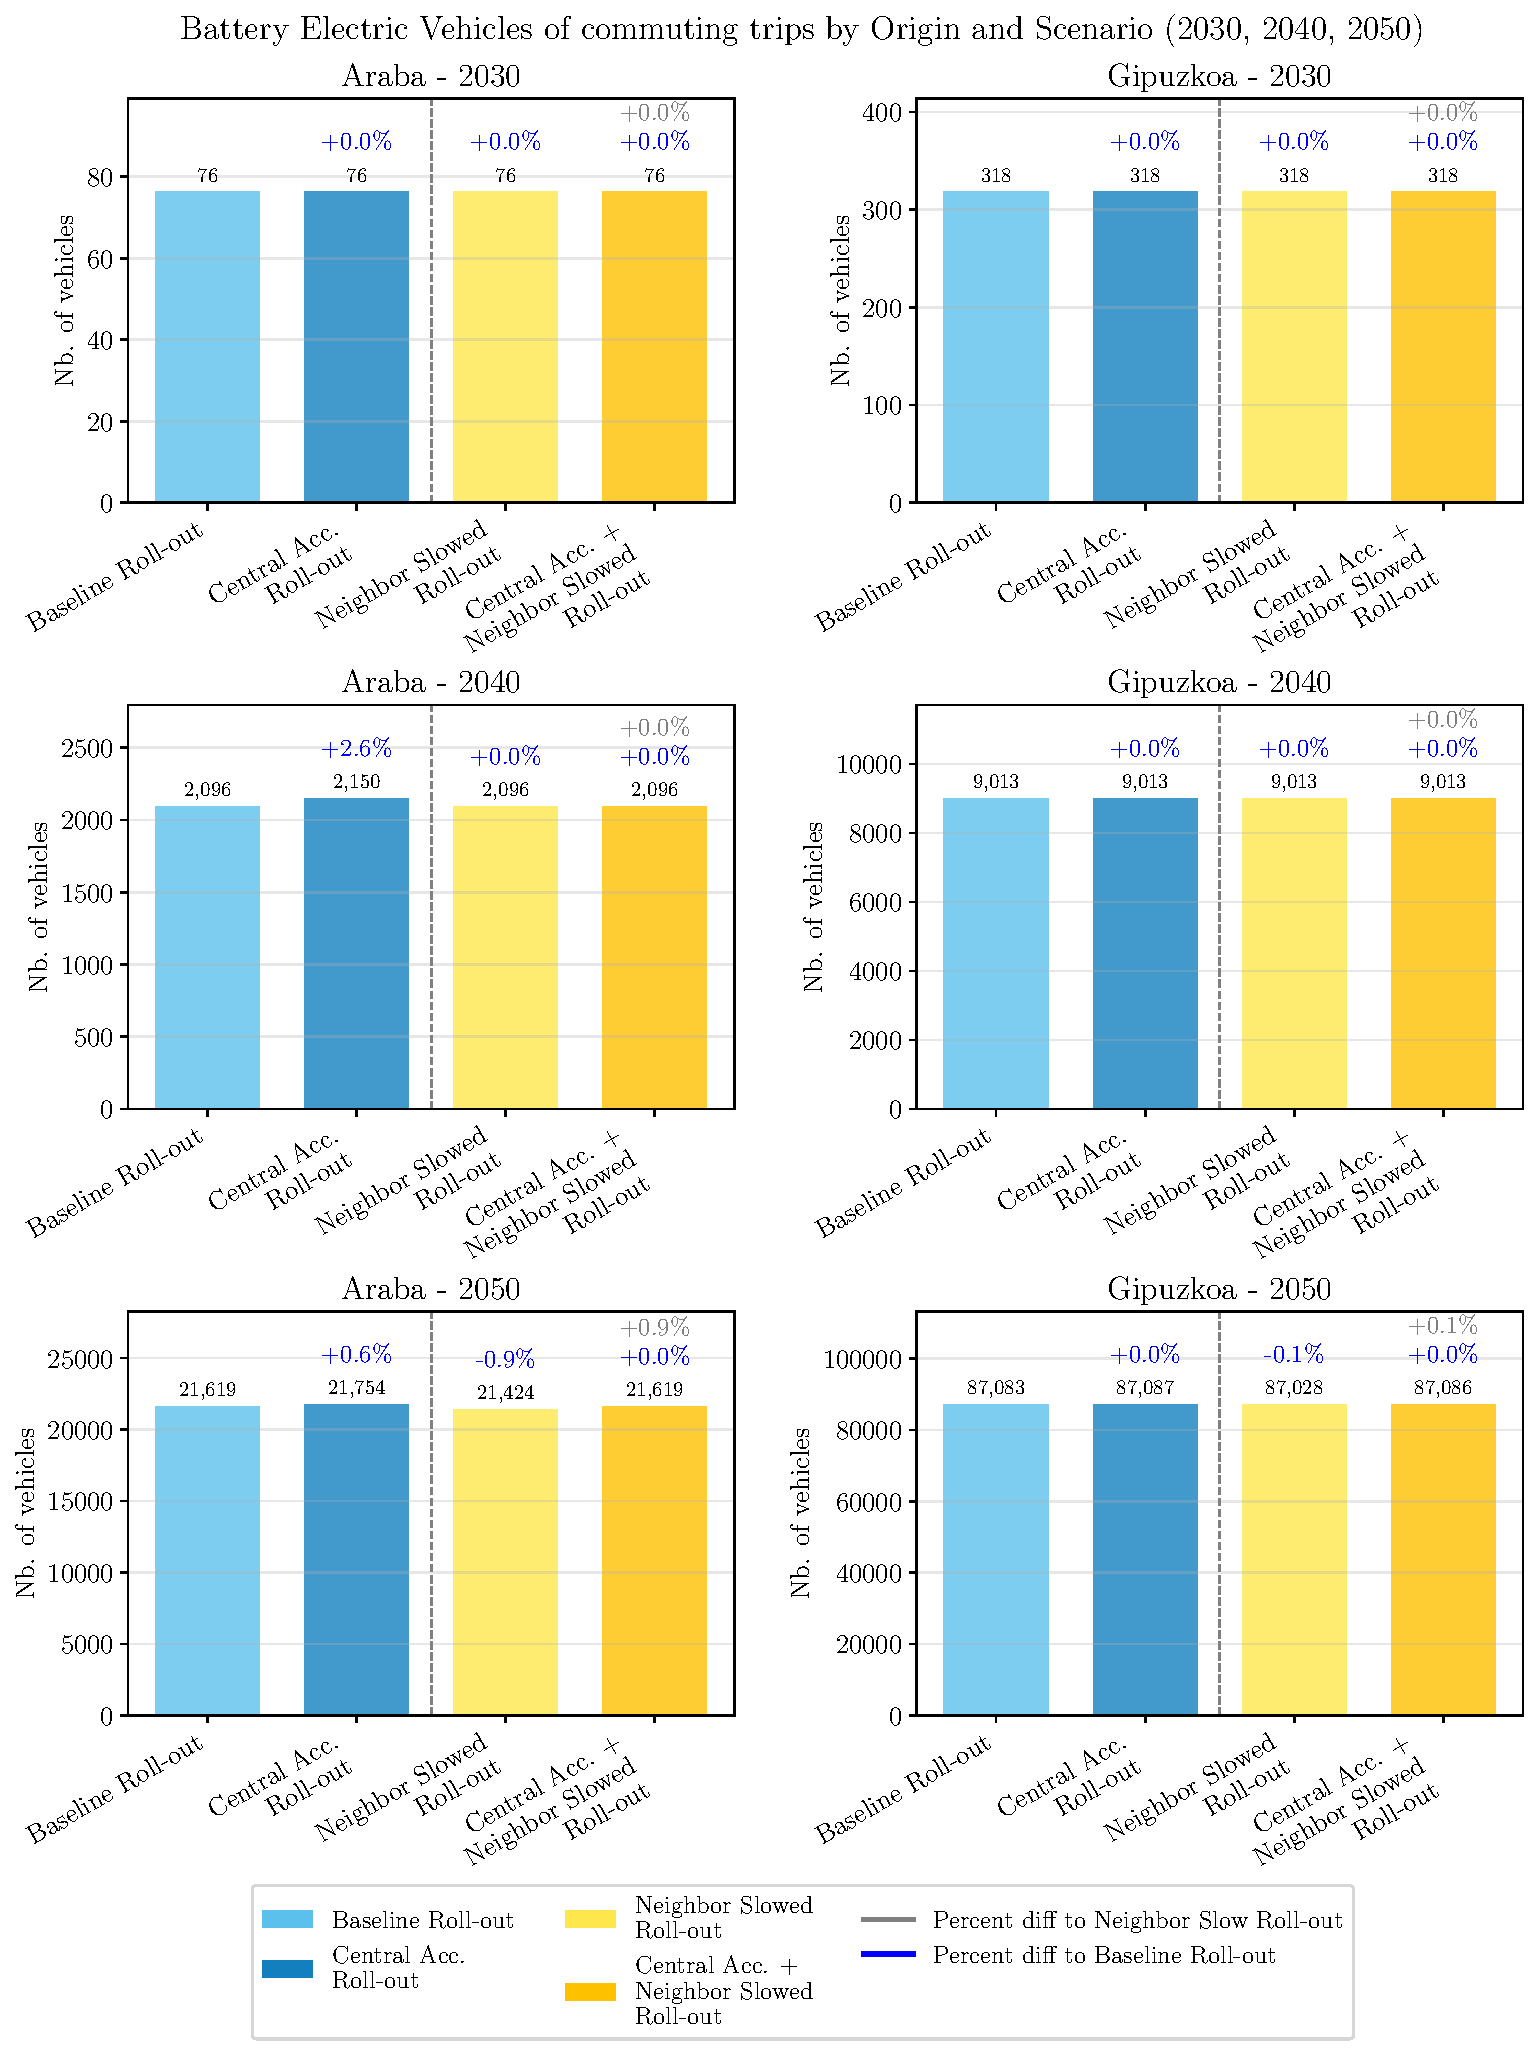
\includegraphics[width=13cm]{graphics/rq2_bevs_by_origin_case_study_2030_2040_2050.pdf}
                \caption{Numbers of BEVs in the commuting trips between Araba or Gipuzkoa and Bizkaia under different scenarios of charging infrastructure roll-out scenarios for years 2030, 2040 and 2050.} \label{fig:rq2_2}
        \end{figure}
 
        \begin{figure}[H]
            \centering
                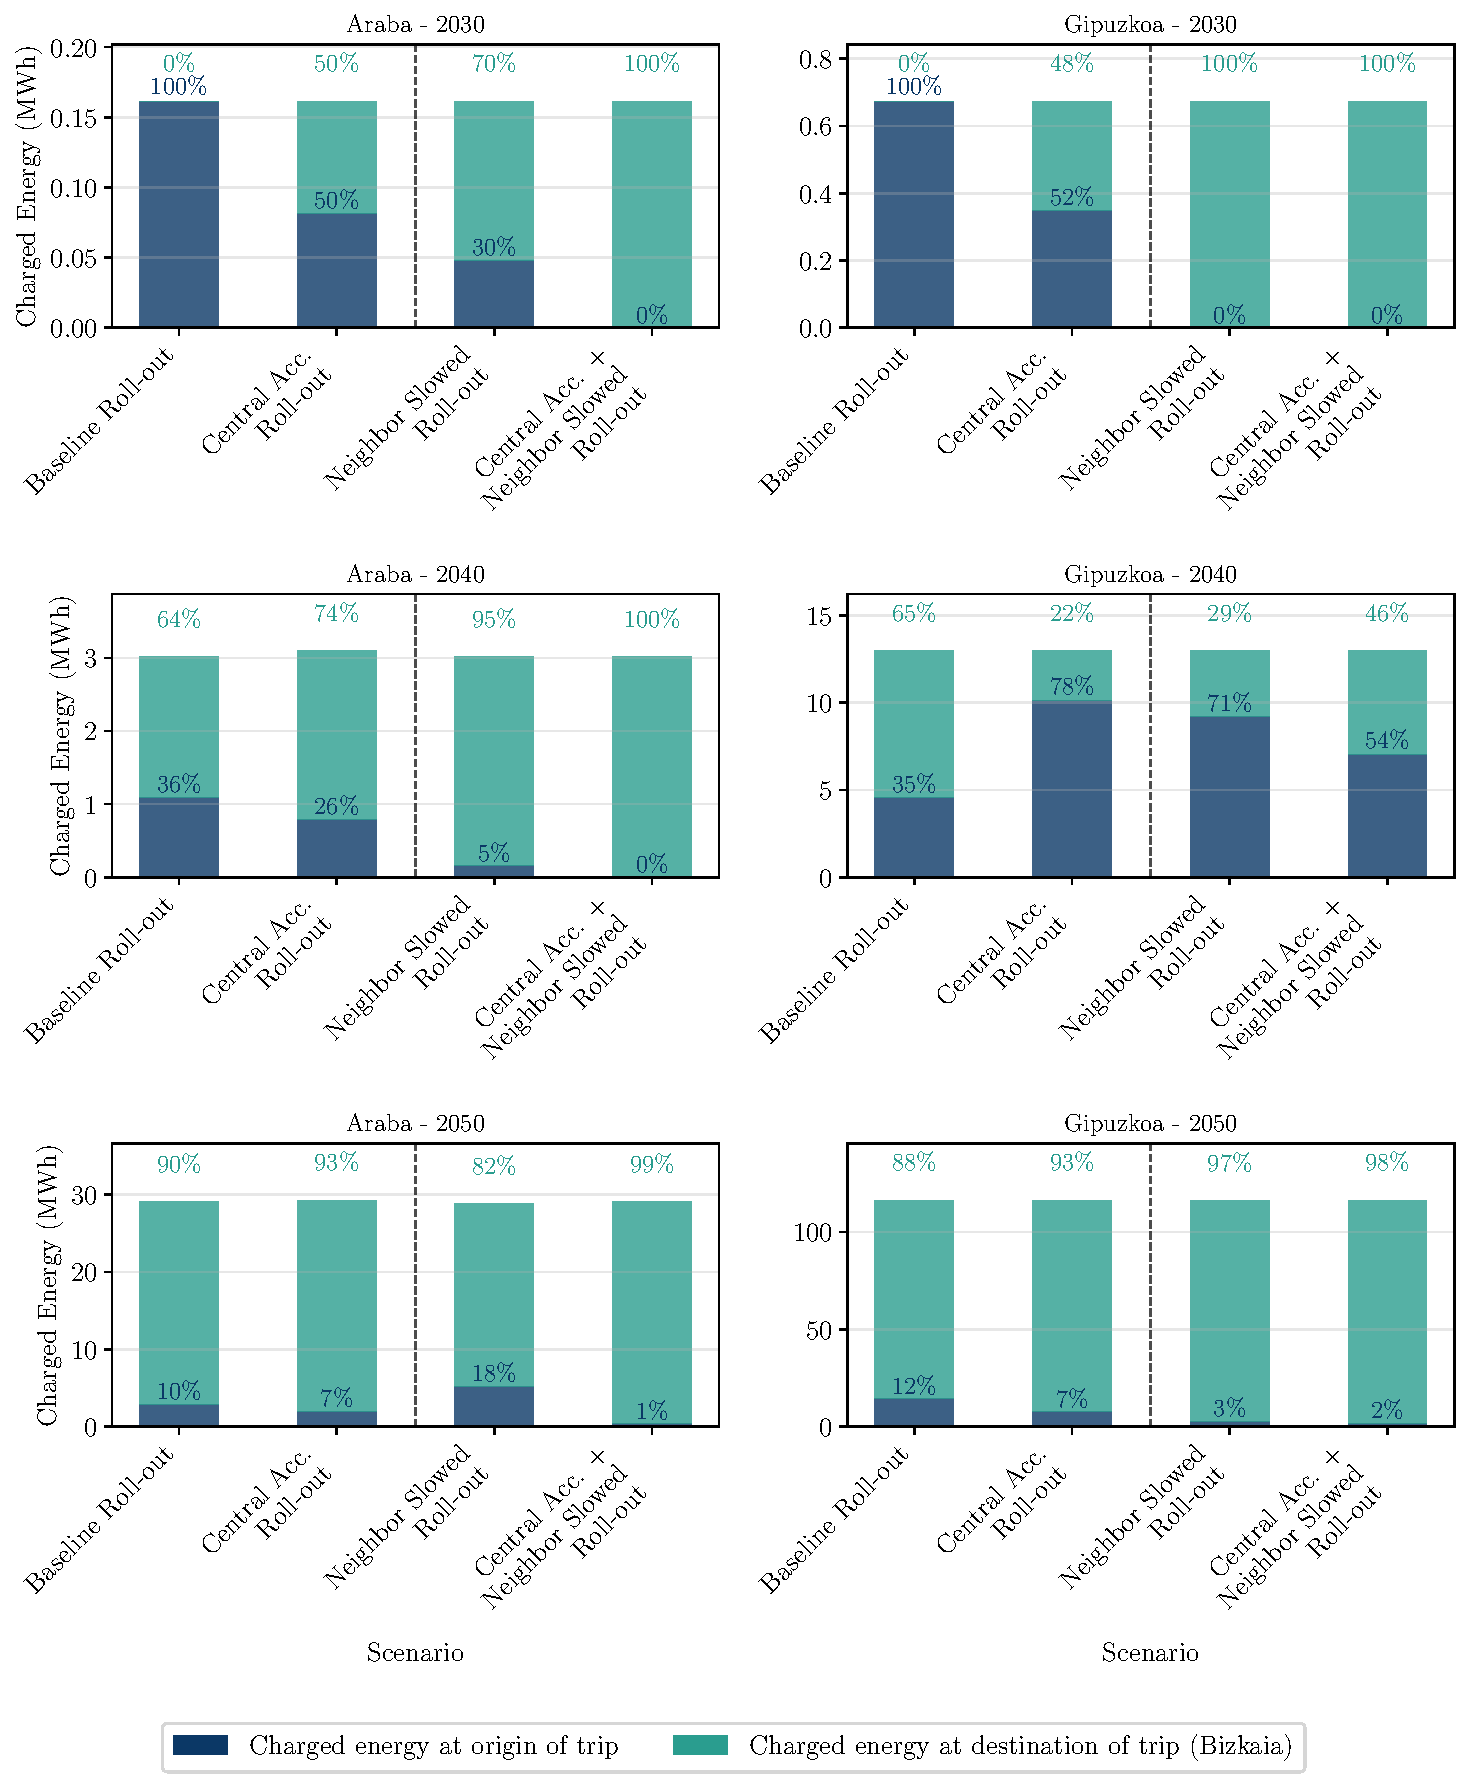
\includegraphics[width=13cm]{graphics/rq2_charged_energy_by_origin_case_subplot.pdf}
                \caption{Snapshots for 2030, 2040 and 2050: Allocation of charging processes between origin and destination of commuting trips originating in Araba or Gipuzkoa and going to Bizkaia with text indicating relative percentages of charging processes.} \label{fig:rq2_3}
        \end{figure}

         \begin{figure}[H]
            \centering
                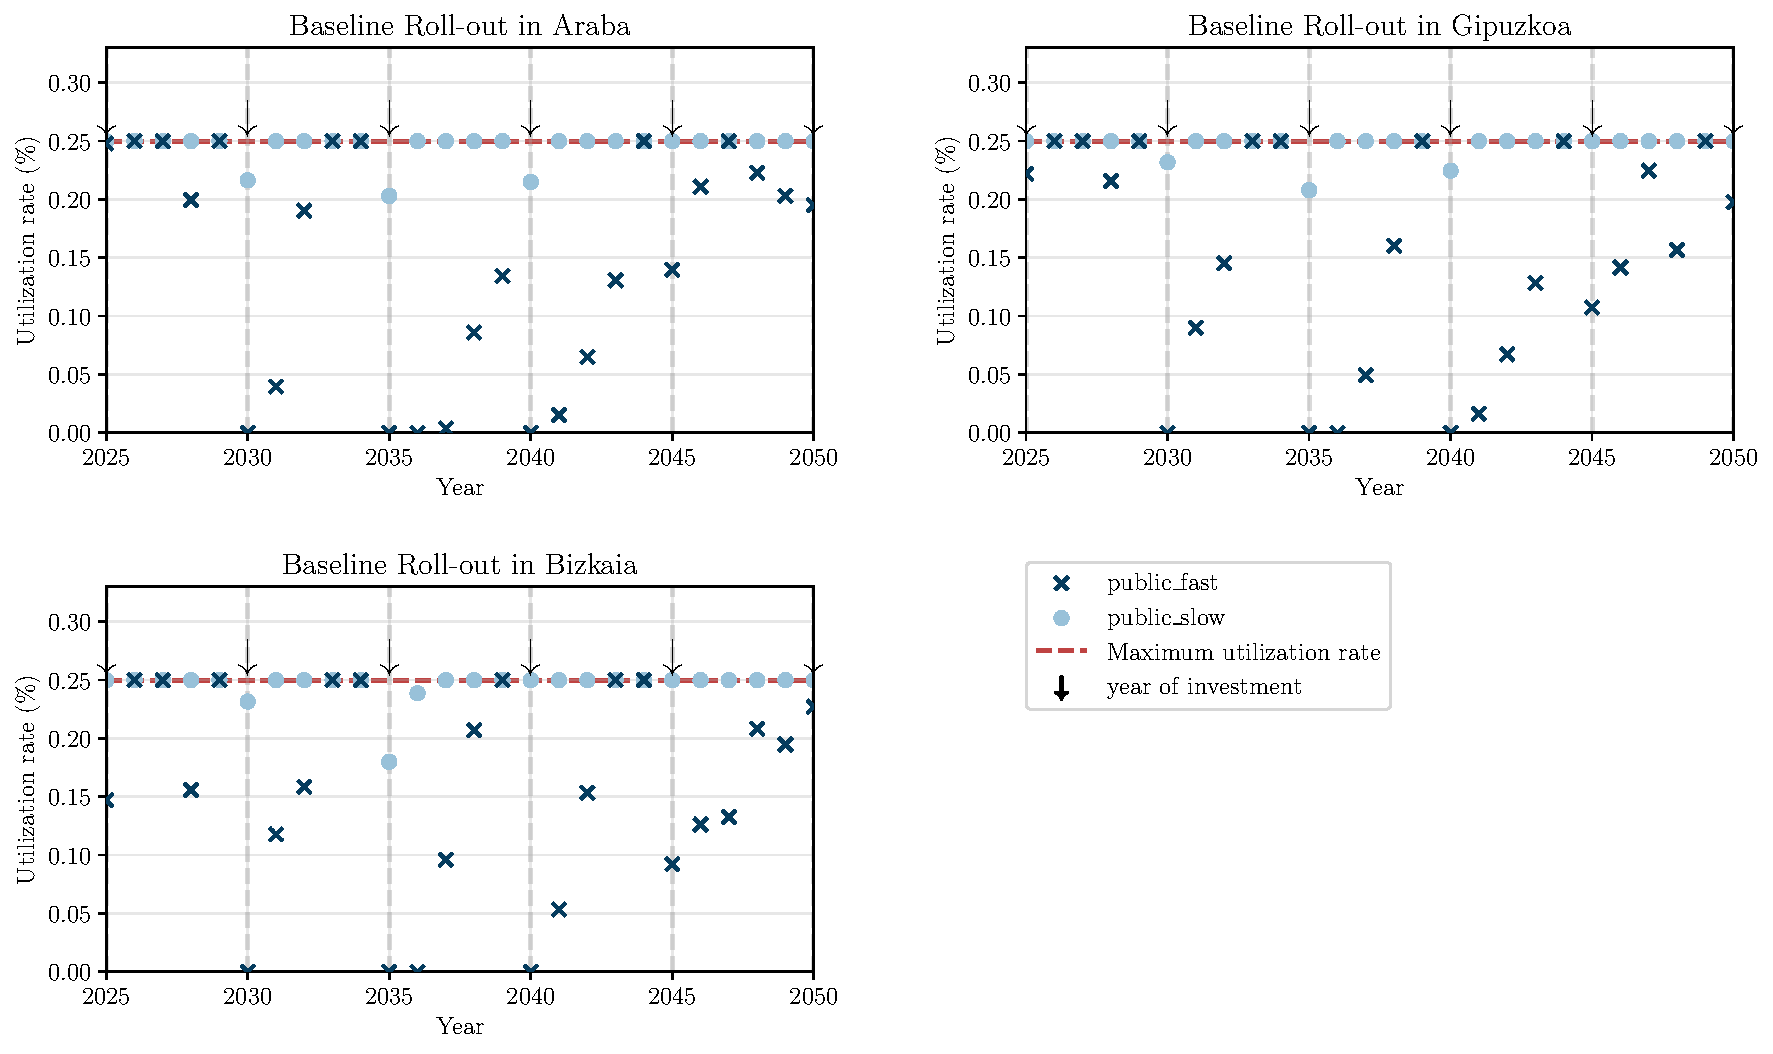
\includegraphics[width=\textwidth]{graphics/rq_2_baseline_utilization_rate.pdf}
                \caption{Development of utilization rates for public charging infrastructure network in Bizkaia, Araba and Gipuzkoa.} \label{fig:rq2_5}
        \end{figure}


    
% \section{Discussion}
   
%     \subsection{The role of income class level differences in high-level charging infrastructure planning}
%     \subsubsection{Indications to charging infrastructure planning}
%     The scenarios for spatial densification of charging infrastructure roll-out lead to different solutions of cost-optimal expansion of infrastructure, the adoption of BEVs across consumer groups, and the allocation of charging processes to different types of chargers.

%     This indicates that the income-class-based differentiation of consumer groups is relevant for charging infrastructure planning and is a relevant dimension to include in methods aiming to model optimal decarbonization pathways for passenger transport. Moreover, the development of the spatial density of a public charger network impacts the usage of different charger types by different consumer groups. This is particularly important during the years of large-scale introduction of BEVs, from 2020 to 2050.

%     Based on our results on this, we deduce the following indications for improving charging infrastructure planning based on the findings of this paper: 
%         \begin{itemize}
%             \item A spatially dense charging infrastructure network can be overall supportive for the decarbonization of different consumer groups of different income levels, but may be in its implementation also hindered by low utilization costs impacting the profitability of the individual investments. This particularly relates to fast charging capacities.
%             \item Consumer groups of lower income classes are less sensitive to long charging times at fast chargers and longer detour times, which is given by the consumer-specific value of time. While we have neglected the high pricing of fast charging processes, our results indicate that longer detouring (an hour of total detouring time for one charging process) and longer charging would not impact the decision to adopt a BEV. This, on the other hand, means that total travel times are substantially prolonged due to the lack of closely allocated and affordable charging infrastructure. 
%             % \item depending on spatial densification; different pathways in the speed of are cost-optimal and allocations of charging processes to different charger types by ic, impacting utilization patterns in the transition process 
%             \item Consumers of the highest income class have the highest sensitivity to time losses due to detouring and fast charging processes. Next to ensuring access to residential charging and a dense charging infrastructure to cover charging demand, available work chargers are an essential supporting lever for ensuring a high level of service.  
%             \item Finally, the allocation of charging processes by charger type changes by scenario of spatial densification throughout all consumer groups. Based on this, it is reasonable to deduce from this that this finally also impacts the utilization pattern of the charging capacity on an hourly level. 
%         \end{itemize}
    

    
%     % We observe a significant impact of the densification strategy in the time frame until 2037. Exclusively, the consumer groups of high income are affected, i.e., early adopters. This time frame overlaps with the years of charging infrastructure expansion, during which detouring times are effectively reduced. The fact that particularly the BEV adoption in higher-income-level consumer groups is affected is in line with the higher weight of the detouring time in the objective function for these income classes through the value of time. While the BEV adoption is only affected in higher-income groups, 

%     \subsubsection{Limitations}
    
%     While public slow charging has a central role in the coverage of the charging demand, public fast charging infrastructure has low utilization rates and is exclusively used by the \textit{Very low income} consumer group. This can be due to two reasons: First, detouring times are systematically higher for public fast charging, and the charging process itself is considered as lost time within the simulation. For the consumer group of very low income, the value of time seems to be sufficiently low so that the time spent on fast charging is not an impaction decrease in the level of service of BEVs. This holds true for all roll-out scenarios. This is in contradiction with empirical research, which indicates high prices in fast-charging \citep{Lanz2022}. Overall, we find that fast charging technology is unfavorable throughout the time of the vehicle stock turnover towards BEVs. 

%     Home charging is not expanded in the optimization. Most likely because it is limited by the monetary budgets of the consumers, and has significantly lower values for the maximum utilization rate (5\%, while values for the other charger types are 20-25\%). This result is not in line with projected home charging capacities that are mostly due to the convenience of home charging, i.e., the reliability for an accessible charging opportunity \citep{STAJIC2023100658}. This consumer-related preference is not sufficiently represented in the present level-of-service approach.
         
%      In the translation of these model-based findings to the implications for charging infrastructure roll-out, the consideration of at least the following limitation of the analysis is important: the function of the relation between the detouring time and capacity expansion is modeled at federal states level and thereby neglects the following aspects: (i) In the formulation of the linking function at NUTS-2 level, we assume an even distribution of charging sites and constant complexity and size of the street network and housing of car owners throughout the modeled area. By doing this, we neglect the different degrees of urbanization and the potential of allocating charging sites at points of interest, which automatically reduces the detouring time significantly in real life. This limitation may lead to an overestimation of the variations in the travel patterns between Araba and Gipuzkoa. (ii) More charging sites with fewer number of charging points does not directly decrease the time needed to reach the closest free charging point. For example, a driver traveling to a charging site with fewer points would need extra time to detour to drive to another charging site, while a larger number of points may prevent this. This is the perspective assumed in the work of \citep{WOLBERTUS2021262}. We assume here that no extra detouring is ever required, i.e. the driver would always know about the state of occupancy before proceeding to travel to the charging site. 
     
%      % Going along with this modeling approach, we automatically assume a negative correlation between the number of charging points per site and detouring time. This must not necessarily be the case. For example, if a driver travels to the closest charging sites, the chances are higher that one of the charging points is available with the presence of a higher number of charging points. \citet{WHITE2022102663} has also found that a higher number of charging points per charging site reduces the possibility of failed charging attempts. When all charging points are occupied, the detouring time increases because the driver needs to travel to another charging site. Therefore, we assume here a full transparency of information exchange on charging station accessibility between charging point operators and the drivers.
     

     
 

  

%      % The utilization rate of fast-charging is overall very low. The limited usage of public fast chargers is most likely due to the charging process being considered within the level of service measure and weighted with the value of time. Therefore, this is not a favorable option to recharge for higher-income classes. Public fast charging capacity is expanded due to the constraint requiring that one-third of the public charging infrastructure needs to be fast-charging. For the value of time by the \textit{Very low income} consumer group, the fast charging is sufficient to cover \hl{\dots} \% of energy demand in 2030 and \hl{\dots} in 2040. In this context, the low value of time causes in the early adoption of charging infrastructure with a higher share of electrified BEVs than \textit{Low income} and \textit{Medium low income} groups. 
     

   

     
     

    

    
     

     
%      % Therefore, how the detouring time to the closest charging infrastructure is does not affect the development of the electrification of the passenger car fleet. hl{Add some sentences in the literature review for the findings of WHITE2022102663, failed charging processes}. This is in contrast to empirical studies that have found significance of the closeness to a charging station \hl{cite here some decision models that have this in it}. 

%      % The detouring time impacts: a little bit of change between cases between the income classes + 

   

     

  


%     \subsection{Spill-over effect of local charging infrastructure investments}
%     \subsubsection{Indications to charging infrastructure planning}
%     The results indicate that the increased charging capacities in Bizkaia impact the adoption in both neighboring regions, Araba and Gipuzkoa. Though this impact is at a small range (maximum 1.3\% added electrification share) and inconsistent among the two regions. 
    
%     This inconsistency in the results between the two regions is most likely due to the variations in the travel patterns of the two regions, which are part of the input data. Observing the adoption in commuting trips versus overall developments of the electrification of the fleets, we deduce that with increased capacities in the destination region, charging processes of commuting trips are allocated at the destination region and make capacities free at the origin region to provide charging capacities for the fleet traveling within the origin region. This statement is also supported by the high utilization rates of public infrastructure.

%     \subsubsection{Limitations}
%     An analytical follow up of this inconsistency requires an expanded methodological setup: On the one hand, a significantly higher amount of analyzed regions; on the other hand, an isolated analysis of commuter traffic, as the present optimization problem determines the cost-optimal development of the charging infrastructure and adoption under constraints that assume a high impact of the global optimum to the individual adoption choice. These constraints include the endogenously set charging capacities as well as constraints related to the maximum rate of total adoption in the passenger fleet.  

%     Overall, the findings are in line with the empirical research on this topic (\citep{QIAN2024104400, SELENASHENG2022103256}) by proving a positive spatial spillover effect. In contrast to the previous literature on this topic, we supplement this branch of research by proving a positive spillover based on techno-economic optimization with the consideration of the comfort of users via the monetization of time. Previous work has proven the evidence of neighboring effects during the early adoption phase, which is also evident in our analysis.
    
    % The charging infrastructure at the destination can only compensate for shortages in charging infrastructure in the neighbouring regions for regular commuting trips. 
    % / is it overestimated? If yes, why? 
    % This impact is primarily given via 

    % trip-based assumption 
    
    % contrast to previous studies / techno-ecomic optimization + convenience via the introduction of value of time measure at this geographic level vs. agent-based higher granularity vs. empirical findings (social aspects) 

    
    % Important discussion points:
    % \begin{itemize}
    %     \item seem to have no impact again on purchase decision in neighbouring countries
    %     \item but impact on charging decision; shifting to neighbouring countries
    %     \item this finding is not in line with previous literature on this, finding indications; these indications in the literature are argued to be based on \dots and \dots; 
    %     \item the personal mindset is often select
    %     \item based on purely techno-economics optimization, this effect does not occur 
    %     \item shift to destination; the approach with charging load and and charging station capacity is represented in a simplified way 
    % \end{itemize}
    % Do these happen?
    % required figures:
    
    
    % \paragraph*{Limitation: trip-based adoption} only a constraint coupling this 
    
    % \begin{enumerate}
    %     \item The difference is how big? how significant is the impact? 
    %     \item Overall quantification of percentage is \dots 
    %     \item Important: Destination charging? What kind is used in the destination charging? Destination charging has a significant role here. 
    % \end{enumerate}
    
    % \textit{Limitations:}
    % \begin{itemize}
    %     % \item \hl{charging prices to better reflect the real costs of charging infrastructure}
    %     \item development of income distribution not considered 
    %     \item urban spatial layout (allocation charging stations) 
    %     \item role of second-hand market vehicle availability 
    %     \item spatial resolution: no peer-based spillover effect 
    %     \item with increased availbility of charging infrastructure: do vehicles decide to reroute and go via this? 
    %     \item what is the model most vulnerable to? 
    %     \item what does a higher initial distribution of charging infrastructure mean? increased parking spots requirements for 
    %     \item Bindeglied BEV adoption = infrastructure detour time,  
    % \end{itemize}
    % important: address here the transferrability of the results 
    % Future work: takling income class related placement on lower geographic level 

\section{Discussion}
   
    \subsection{The role of income class level differences in high-level charging infrastructure planning}
    \subsubsection{Indications to charging infrastructure planning}
    The scenarios for spatial densification of charging infrastructure roll-out lead to different solutions of cost-optimal expansion of infrastructure, the adoption of BEVs across consumer groups, and the allocation of charging processes to different types of chargers.

    This indicates that the income-class-based differentiation of consumer groups is relevant for charging infrastructure planning and is a relevant dimension to include in methods aiming to model optimal decarbonization pathways for passenger transport. Moreover, the development of the spatial density of a public charger network impacts the usage of different charger types by different consumer groups. This is particularly important during the years of large-scale introduction of BEVs, from 2020 to 2050.

    Based on our results on this, we deduce the following indications for improving charging infrastructure planning based on the findings of this paper: 
        \begin{itemize}
            \item A spatially dense charging infrastructure network can be overall supportive for the decarbonization of different consumer groups of different income levels, but may\added{also }be\added{ hindered} in its implementation\deleted{also hindered} by low utilization costs impacting the profitability of the individual investments. This particularly relates to fast charging capacities.
            \item Consumer groups of lower income classes are less sensitive to long charging times at fast chargers and longer detour times, which is given by the consumer-specific value of time. \footnote{\added{This finding reflects the assumed VoT values and should be interpreted as a model-conditional outcome rather than an empirically validated behavioral pattern.}} While we have \replaced{not considered}{neglected} the high pricing of fast charging processes, our results indicate that longer detour\deleted{ing} (an hour of total detouring time for one charging process) and longer charging would not impact the decision to adopt a BEV. This, on the other hand, means that total travel times are substantially prolonged due to the lack of closely allocated and affordable charging infrastructure. 
            % \item depending on spatial densification; different pathways in the speed of are cost-optimal and allocations of charging processes to different charger types by ic, impacting utilization patterns in the transition process 
            \item Consumers of the highest income class have the highest sensitivity to time losses due to detouring and fast charging processes. \replaced{In addition}{Next} to ensuring access to residential charging and a dense charging infrastructure to cover charging demand, available work chargers are an essential supporting lever for ensuring a high level of service.  
            \item Finally, the allocation of charging processes by charger type changes by scenario of spatial densification throughout all consumer groups. Based on this, it is reasonable to deduce \deleted{from this }that this\deleted{ finally} also impacts the utilization pattern of the charging capacity on an hourly level. 
        \end{itemize}
    

    
    % We observe a significant impact of the densification strategy in the time frame until 2037. Exclusively, the consumer groups of high income are affected, i.e., early adopters. This time frame overlaps with the years of charging infrastructure expansion, during which detouring times are effectively reduced. The fact that particularly the BEV adoption in higher-income-level consumer groups is affected is in line with the higher weight of the detouring time in the objective function for these income classes through the value of time. While the BEV adoption is only affected in higher-income groups, 

    \subsubsection{Limitations} \label{sec:lim_1}
    
    While public slow charging has a central role in the coverage of the charging demand, public fast charging infrastructure has low utilization rates and is exclusively used by the \textit{Very low income} consumer group. This can be due to two reasons: First, detouring times are systematically higher for public fast charging, and the charging process itself is considered as lost time within the simulation. For the consumer group of very low income, the value of time seems to be sufficiently low so that the time spent on fast charging is not an \replaced{impactful}{impaction} decrease in the level of service of BEVs. This holds true for all roll-out scenarios. This is in contradiction with empirical research, which indicates high prices \replaced{for}{in} fast-charging \cite{Lanz2022}. \added{The consideration of a cost markup for fast charging would most probably reduce the cost-effectiveness of the fast charger utilization which would lead to reduced or no fast charging and shift the charging demand to public slow chargers. Consequently, the finding that \textit{Very low income} consumers predominantly use fast charging should be interpreted as a model outcome under cost-minimization assumptions rather than a behavioral prediction, and this pattern would likely reverse under realistic pricing structures.} Overall, we find that fast charging technology is unfavorable throughout the time of the vehicle stock turnover towards BEVs. 

    Home charging is not expanded in the optimization. Most likely because it is limited by the monetary budgets of the consumers, and has significantly lower values for the maximum utilization rate (5\%, while values for the other charger types are 20-25\%). This result is not in line with projected home charging capacities that are mostly due to the convenience of home charging, i.e., the reliability for an accessible charging opportunity \cite{STAJIC2023100658}. This consumer-related preference is not sufficiently represented in the present level-of-service approach.
         
     In the translation of these model-based findings to the implications for charging infrastructure roll-out, the consideration of at least the following limitation of the analysis is important: the function of the relation between the detouring time and capacity expansion is modeled at federal states level and thereby neglects the following aspects: (i) In the formulation of the linking function at NUTS-2 level\footnote{\added{Results of sensitivity analyses on the detour fueling time reduction function are presented in Section \ref{sec:app_spatialdens}}.}, we assume an even distribution of charging sites and constant complexity and size of the street network and housing of car owners throughout the modeled area. By doing this, we neglect the different degrees of urbanization and the potential of allocating charging sites at points of interest, which automatically reduces the detouring time significantly in real life. \deleted{This limitation may lead to an overestimation of\deleted{ the} variations in the travel patterns between Araba and Gipuzkoa.} (ii) More charging sites with\added{ a} fewer number of charging points does not directly decrease the time needed to reach the closest free charging point. For example, a driver traveling to a charging site with fewer points would need extra time to \replaced{drive}{detour} to drive to another charging site, while a larger number of points may prevent this. This is the perspective assumed in the work of \cite{WOLBERTUS2021262}. We assume here that no extra detouring is ever required, i.e.\added{,} the driver would always know about the state of occupancy before proceeding to travel to the charging site.

        \subsection{Spill-over effect of local charging infrastructure investments}
    \subsubsection{Indications to charging infrastructure planning}
    The results indicate that the increased charging capacities in Bizkaia impact the adoption in both neighboring regions, Araba and Gipuzkoa. \replaced{However,}{Though} this impact is at a small range (maximum \replaced{2.1\%}{1.3\%} added electrification share) and inconsistent \replaced{between}{among} the two regions. 
    
    This inconsistency in the results between the two regions is most likely due to the variations in the travel patterns of the two regions, which are part of the input data. Observing the adoption in commuting trips versus overall developments of the electrification of the fleets, we deduce that with increased capacities in the destination region, charging processes of commuting trips are allocated at the destination region and \replaced{free up}{make} capacities\deleted{ free} at the origin region to provide charging capacities for the fleet traveling within the origin region. This statement is also supported by the high utilization rates of public infrastructure.

    \subsubsection{Limitations} \label{sec:lim_2}
    An analytical follow\added{-}up of this inconsistency requires an expanded methodological setup: On the one hand, a significantly higher amount of analyzed regions; on the other hand, an isolated analysis of commuter traffic, as the present optimization problem determines the cost-optimal development of the charging infrastructure and adoption under constraints that assume a high impact of the global optimum \replaced{on}{to} the individual adoption choice. These constraints include the endogenously set charging capacities as well as constraints related to the maximum rate of total adoption in the passenger fleet.  
    \added{An important limitation that would very likely impact the observations here, is the assumptions made about the absolute amounts of commuter trips. The data we use is based on the calibration of car trip numbers for the year 2010 within the ETISplus project \cite{ETISplus_233596}. Due to the lack of knowledge on the developments of commuter traffic and passenger trips for other purposes, we assume a constant increase according to GDP over all types of car trips. Though, it is important to note here, that the results heavily dependent on the assumed number of commuting trips between the regions. Moreover, there is an uncertainty containing the trip lengths assigned to the regional trips, as these are not drawn from a mobility study conducted in Austria.} 
    Overall, the findings are in line with the empirical research on this topic (\cite{QIAN2024104400, SELENASHENG2022103256}) by proving a positive spatial spillover effect. In contrast to the previous literature on this topic, we supplement this branch of research by proving a positive spillover based on techno-economic optimization with the consideration of the comfort of users via the monetization of time. Previous work has proven the evidence of neighboring effects during the early adoption phase, which is also evident in our analysis.
    \added{The limitations discussed here and in Section \ref{sec:lim_1} are subject to future work}.
    
\section{Conclusion}

    When planning a charging infrastructure network while considering different consumer groups, previous scientific literature emphasizes taking into account consumers of various housing types. Our results have shown that, in addition, the differentiation by income classes is relevant: \added{building on income-class-specific value of time assumptions,} the income class of consumers influences the utilization patterns of the charging network. Furthermore, the spatial density of the public charging infrastructure network affects these utilization patterns and the associated optimal design of the charging capacities.
    
    While previous empirical research has proven a positive spatial spill\deleted{-}over effect of local charging infrastructure expansion on the BEV adoption of early adopters in neighboring regions, our analysis has shown the potential of this based on system-techno-economic-optimality in the long-term. Although the observed impact is small, as a 30\% increase in local charging capacity has a maximum impact of \replaced{2.1}{1.3}\% on the BEV adoption in the neighboring region. 

    \added{Future work must focus on tackling the limitations this work (as discussed in Sections \ref{sec:lim_1} and \ref{sec:lim_2}).} \added{Further,} \replaced{p}{P}art of future work must be an improved representation of consumer-group-specific monetary constraints, particularly with regard to operating costs, as well as the connection of the dimensions of different income levels with housing types to improve the representation of utilization patterns and the planning of capacities. \added{Additionally, extending the model to sub-annual temporal resolution would enable representation of peak-hour charging behavior and queuing dynamics.} Moreover, future work should still continue to closely analyze spatial cross-regional impacts. On the one hand, further analysis should be conducted to examine the effects at geographic aggregation levels where higher amounts of cross-border commuting trips are present, for example, at the municipality or neighborhood level. \added{Higher cross-border interactions could be also studied by different case studies similar geographic scope and granularity.} Furthermore, such analysis should also include a potential detour to other neighborhoods for the purpose of recharging, while considering the consumer-group-dependent value of time.
    

    % In planning charging infrastructure for the purpose of supporting the growth of the passenger BEV fleet beyond the early adoption stage, the spatially dense coverage of public slow chargers is particularly important for pushing the adoption in consumer groups of high to medium income levels. Further, to ensure high utilization of fast chargers, the need to install these near points of interest are essential in the long-term. A spatially dense public slow charging infrastructure can support the BEV adoption not only locally but beyond region borders and, in particular, the adoption of BEVs in the commuting passenger car fleet. 

    % The consideration of different income classes is relevant to deducing charging patterns. Further, this can be enhanced by introducing parameters in analyses of a higher spatial scale by considering a measure, such as the detouring time, to introduce the parameter of spatial density. Going forward, the accurate consideration of these income-class-related differences requires a dynamic representation between hourly demand patterns based on consumer behavior and charging infrastructure planning.   





\section{CRediT authorship contribution statement}

\textbf{Antonia Golab:} Conceptualization, Methodology, Software, Validation, Formal analysis, Writing - Original Draft, Visualization.  
\textbf{Sebastian Zwickl-Bernhard:} Conceptualization, Methodology, Writing - Review \& Editing.  
\textbf{Marcus Otti:} Conceptualization, Writing - Review \& Editing.  
\textbf{Hans Auer:} Conceptualization, Methodology, Writing - Review \& Editing, Supervision, Funding acquisition.


\section{Acknowledgments}
This work was financially supported by the iDesignRES research project which is funded by the European Union’s Horizon Europe Research and Innovation Programme under grant agreement No. 101095849.  
The authors acknowledge TU Wien Bibliothek for financial support through its Open Access Funding Programme.

\section{Declaration of generative AI and AI-assisted technologies in the writing process.}
During the preparation of this work the authors used DeepL, Grammerly\added{, Claude} and ChatGPT in order to avoid spelling errors in the manuscript. After using this tool/service, the authors reviewed and edited the content as needed and takes full responsibility for the content of the published article.
\bibliographystyle{elsarticle-harv}
\bibliography{literature}
\appendix

\section{Methodology and Data (extended)} 

\label{sec: extended_math_form}
\subsection{Mathematical formulation (extended)}
% \begin{longtable}{llll}
% \caption{Nomenclature}
% \label{tab:nomenclature}\\
% \hline
% Sets and indices                         & Description                                                          &         &               \\ \hline
% \endfirsthead
% %
% \endhead
% %
% \hline
% \endfoot
% %
% \endlastfoot
% %
% $y \in \mathcal{Y}$                      & year                                                                 &         &               \\

% $u \in \mathcal{U}$                      & consumer group                                                           &         &               \\
% $p \in \mathcal{P}$                      & trip purpose                                                         &         &               \\
% $r \in \mathcal{R}_p$                      & trip between origin-destination (OD) pair for a specified purpose                                        &         &               \\
% $k \in \mathcal{K}$                      & travel paths                                                         &         &               \\

% $e \in \mathcal{E}$                      & geographic location                                                  &         &               \\
% $v \in \mathcal{V}$                      & type of vehicle                                                      &         &               \\
% $t \in \mathcal{T}_v$                      & drive-train technology fueled by a specific fuel                     &         &               \\
% $g \in \mathcal{G}$                      & year that vehicle was introduced to market                           &         &               \\
% $l \in \mathcal{L}$                      & types of fueling infrastructure (by max. power output at allocation) &         &               \\
% $i \in \mathcal{I}^l$ & index for detour time reduction potential for type of fueling infrastructure $l$& \\
% $\mathcal{Y}^{exp}$                      & set of years of investment decisions                                 &         &               \\
% $\mathcal{L}^{not home}$ &
%   fueling infrastructure that is not allocated at home of vehicle owner &
%    &
%    \\
   
%    $\mathcal{L}^{home}$ &
%   fueling infrastructure that is allocated at home of vehicle owner &
%    &
%    \\
%    $\mathcal{L}_{tk}$ & types of infrastructure by drive-train technology and availability for travel path & & \\
%    $\mathcal{E}_{kl}$ & geographic location along travel path and available fueling type & & \\\hline
% Decision variables                       &                                                                      & Unit    &               \\ \hline
% $f_{yurkvtg}$                           & number of trips                                                      &         & $[0,\infty[$  \\
% \textbf{$h_{yurkvtg}$}                  & number of vehicles                                                   &         & $[0, \infty[$ \\
% $h^{+}_{yurkvtg}$                       & newly purchased vehicles                                             &         & $[0,\infty[$  \\
% $h^{-}_{yurkvtg}$                       & number of vehicles leaving the vehicle stock                         &         & $[0, \infty[$ \\
% $s_{yurkvtgle}$                         & energy fueled                                                        & kWh     & $[0, \infty[$ \\
% $n_{yurkvtgle}$               & number of fueling vehicles                                           &         & $[0, \infty[$ \\
% $b_{yurkvtle}$ &
%   \begin{tabular}[c]{@{}l@{}}fueling detour time to reach closest available public charging \\ infrastructure\end{tabular} &
%   h &
%   $[0, \infty[$ \\
% $w_{eli}$ &
%   \begin{tabular}[c]{@{}l@{}}binary decision variable indicating whether detour reduction $i$ is\\ active\end{tabular} &
%    &
%   $\{ 0, 1\}$ \\
% $z_{yrkvtle,i}$ &
%   decision variable substituting the multiplication $b* w$ &
%   h &
%   $[0, \infty]$ \\
% $q^{+,\mathrm{fuel\_infr, home}}_{yrte}$ & added fueling infrastructure at home                                 & kW      & $[0,\infty[$  \\
% $q^{+, \mathrm{fuel\_infr}}_ {ytle}$               & added fueling infrastructure                                         & kW      & $[0, \infty[$ \\
% $\mathrm{budget}^{+}_{yur}$              & budget overrun                                                       & \euro   & $[0, \infty[$ \\
% $\mathrm{budget}^{-}_{yur}$              & budget underrun                                                      & \euro   & $[0, \infty[$ \\ \hline
% Parameters                               &                                                                      &         &               \\ \hline
% $\mathrm{LoS}$                           & level of service                                                     & h       &               \\
% $\mathrm{VoT}$                           & value of time                                                        & \euro/h &               \\
% $\gamma_l$                               & factor between                                                                &         &               \\
% $Q^{\mathrm{fuel_infr, not home}}_{urte}$         & Initial fueling infrastructure at home                               & kW      &               \\
% $Q^{\mathrm{fuel_infr, home}}_{urtle}$                       & Initial fueling infrastructure                                        & kW      &               \\
% $\hat{Q}^{\mathrm{max}}_{yule}$                & Upper limit for charging infrastructure capacity by consumer group                    & kW      &               \\
% $\hat{Q}^{\mathrm{max}}_{yle}$                & Upper limit for charging infrastructure capacity                    & kW      &               \\
% $\alpha_{eli}$                           & reduction $i = 1, \dots, I$ of detour time                           & \%      &               \\
% $\tau^u$                                 & investment periods in new vehicle                                          &         &               \\
% $B^{\mathrm{init}}_{el}$                          & initial detour time                                                  &         &  h             \\
% $D^{\textrm{spec}}_{vtg}$                         & specific energy consumption                                          & kWh/km  &               \\
% $W_{vtg}$                                & load factor                                                          &  persons/vehicle       &               \\
% $\mathrm{Cap}^{\mathrm{tank}}_{vtg}$ & tank capacity & kWh& \\
% $L^{annual}_{vtg}$ & annual range & km & \\
% $L_{k}$                                  & length of path                                                       & km      &               \\ 
% $\mathrm{Budget}_u$ & monetary budget of consumer group& & €/trip \\\hline
% \end{longtable}

\begin{scriptsize}
\begin{longtable}{llll}
\caption{Nomenclature (extended).}
\label{tab:nomenclature_main}\\
\hline
Sets and indices                         & Description                                                          &         &               \\ \hline
\endfirsthead
%
\endhead
%
\hline
\endfoot
%
\endlastfoot
%
$y \in \mathcal{Y}$                      & year                                                                 &         &               \\
$u \in \mathcal{U}$                      & consumer group                                                       &         &               \\
$p \in \mathcal{P}$                      & trip purpose                                                         &         &               \\
$r \in \mathcal{R}_p$                    & trip between origin-destination (OD) pair for a specified purpose    &         &               \\
$k \in \mathcal{K}$                      & travel paths                                                         &         &               \\
$e \in \mathcal{E}$                      & geographic location                                                  &         &               \\
$v \in \mathcal{V}$                      & type of vehicle                                                      &         &               \\
$t \in \mathcal{T}_v$                    & drive-train technology fueled by a specific fuel                     &         &               \\
$g \in \mathcal{G}$                      & year that vehicle was introduced to market                           &         &               \\
$l \in \mathcal{L}$                      & types of fueling infrastructure (by capacity)                        &         &               \\
$i \in \mathcal{I}_l$ &  \multicolumn{3}{l}{index for detour time reduction potential for type of fueling infrastructure $l$ }\\
$\mathcal{Y}^{exp}$                      & set of years of investment decisions                                 &         &               \\
$\mathcal{K}_{e}$                        & set of paths that go through edge $e$                                &         &               \\
$\mathcal{L}^{not home}$ & \multicolumn{3}{l}{fueling infrastructure that is not allocated at home of vehicle owner} \\
$\mathcal{L}^{home}$ & fueling infrastructure that is allocated at home of vehicle owner & & \\
$\mathcal{L}_{tk}$ & \multicolumn{3}{l}{types of infrastructure by drive-train technology and availability for travel path} \\
$\mathcal{E}_{kl}$ & geographic location along travel path and available fueling type & & \\
$S^u_j$ & \multicolumn{3}{l}{\begin{tabular}[t]{@{}l@{}}$ = \{ y_m \in Y | j \in [m, m + \tau_u -1]\}, m=1, ..., |Y| -\tau _u +1 $ \\ subsets of time periods for which a monetary budget is defined by consumer group\end{tabular}}   \\
\\\hline
Decision variables                       &                                                                      & Unit    &               \\ \hline
$f_{yurkvtg}$                           & number of person-trips                                               & -       & $[0,\infty[$  \\
\textbf{$h_{yurkvtg}$}                  & number of vehicles                                                   & -       & $[0, \infty[$ \\
$h^{+}_{yurkvtg}$                       & newly purchased vehicles                                             & -       & $[0,\infty[$  \\
$h^{-}_{yurkvtg}$                       & number of vehicles leaving the vehicle stock                         & -       & $[0, \infty[$ \\
$s_{yurkvtgle}$                         & energy fueled                                                        & kWh     & $[0, \infty[$ \\
$n_{yurkvtgle}$                         & number of fueling vehicles                                           &         & $[0, \infty[$ \\
$b_{yurkvtle}$ & \begin{tabular}[t]{@{}l@{}}fueling detour time to reach closest available public charging \\ infrastructure\end{tabular} & h & $[0, \infty[$ \\
$w_{yeli}$ & \begin{tabular}[t]{@{}l@{}}binary decision variable indicating whether detour reduction $i$ is\\ active\end{tabular} & - & $\{ 0, 1\}$ \\
$z_{yrkvtle,i}$ & decision variable substituting the multiplication $b* w$ & h & $[0, \infty[$ \\
$q^{+,\mathrm{fuel\_infr, home}}_{yrte}$ & added fueling infrastructure at home                                 & kW      & $[0,\infty[$  \\
$q^{+, \mathrm{fuel\_infr}}_ {ytle}$     & added fueling infrastructure                                         & kW      & $[0, \infty[$ \\
$q^{\Delta +, \mathrm{fuel\_infr}}_ {ytle}$ & \begin{tabular}[t]{@{}l@{}}relative difference of fueling capacity expansion to fixed capacity \\ size values $cap$\end{tabular} & kW & $[0, \infty[$ \\
$\mathrm{budget}^{+}_{yur}$              & budget overrun                                                       & \euro   & $[0, \infty[$ \\
$\mathrm{budget}^{-}_{yur}$              & budget underrun                                                      & \euro   & $[0, \infty[$ \\ \hline
Parameters                               &                                                                      &         &               \\ \hline
$\mathrm{LoS}$                           & level of service                                                     & h       & $[0, \infty[$ \\
$\mathrm{VoT}$                           & value of time                                                        & \euro/h & $[0, \infty[$ \\
$\gamma_l$                               & factor between annual peak hour and total annual demand              & \%      & $[0, 100]$ \\
$Q^{\mathrm{fuel_infr, not home}}_{urte}$ & Initial fueling infrastructure at home                               & kW      & $[0, \infty[$ \\
$Q^{\mathrm{fuel_infr, home}}_{urtle}$   & Initial fueling infrastructure                                       & kW      & $[0, \infty[$ \\
$\hat{Q}^{\mathrm{max}}_{yule}$          & upper limit for charging infrastructure capacity by consumer group   & kW      & $[0, \infty[$ \\
$\hat{Q}^{\mathrm{max}}_{yle}$           & upper limit for charging infrastructure capacity                     & kW      & $[0, \infty[$ \\
$\alpha_{iel}$                           & reduction $i = 1, \dots, I$ of detour time                           & \%      & $[0, 100]$ \\
$cap_{eli}$ & \begin{tabular}[t]{@{}l@{}}fixed lower bounds for capacity which tie to a reduction of\\ detour time of $\alpha_{i}$  \end{tabular} & kWh & $[0, \infty[$ \\
$\tau^u$ & \begin{tabular}[t]{@{}l@{}}number of years between consecutive vehicle purchase decisions, \\representing the vehicle replacement period\end{tabular} & a & $[0, \infty[$ \\
$\beta$                                 & relative threshold for budget under- or overrun                      & \%      & $[0, 100]$ \\
$B^{\mathrm{init}}_{el}$                 & initial detour time                                                  & h       & $[0, \infty[$ \\
$D^{\textrm{spec}}_{vtg}$                & specific energy consumption                                          & kWh/km  & $[0, \infty[$ \\
$W_{vtg}$                                & load factor                                                          & persons/vehicle & $[0, \infty[$ \\
$\mathrm{Cap}^{\mathrm{tank}}_{vtg}$     & tank capacity                                                        & kWh     & $[0, \infty[$ \\
$L^{annual}_{vtg}$                       & annual range                                                         & km      & $[0, \infty[$ \\
$L_{k}$                                  & length of path                                                       & km      & $[0, \infty[$ \\
$C^{\mathrm{CAPEX}}_{yvtg}$              & expenditure costs for vehicles                                       & -       & $[0, \infty[$ \\
$\mathrm{Budget}_u$                      & monetary budget of consumer group                                    & \euro/trip & $[0, \infty[$ \\
\hline
\end{longtable}
\end{scriptsize}

\textit{appendix} Decision variable $f$ expresses the number of trips covered by a specific vehicle type and technology-fuel pair of a specific generation. The sum over all possible travel paths, vehicle types, technology-fuel pairs and vehicle generations equals the exogenously given travel demand:  


          \begin{equation} \label{equ:demand_cov}
                \begin{split}
                    \sum_{k \in \mathcal{K}_r} \sum_{v \in V} \sum_{t \in \mathcal{T}_v} \sum_{g \in \mathcal{G}} f_{yurkvtg} = F_{yur} \quad :  \forall y, u, r
                \end{split}
            \end{equation}
        
         \textit{appendix} The right side of the equation expresses the coverage of the demand by different vehicle types and drive-train technologies of different generations.

        \textit{appendix} Based on the trips covered by a vehicle type of a technology, the vehicle stock is sized as follows:
        
        \begin{flalign} \label{equ:fleet_size_demand}
        \begin{split}
             h_{yurvtg} \geq \sum_{k \in \mathcal{K}_r}\frac{L_{k}}{W_{yvtg} L^{\mathrm{annual}}_{vtg}} f_{yurkvtg} \quad :\forall y,u,r,k,v,t,g
        \end{split}
    \end{flalign}

    \begin{flalign} \label{equ:fleet_size_change_1}
        \begin{split}
             \sum_{p} h_{yurvtg} = \sum_{p} h_{(y-1)rvtg} + \sum_{p} h^{+}_{yurvtg} - \sum_{p} h^{-}_{yurvtg} \quad :\forall y\in \mathcal{Y}\setminus{\{0\}},u,r,v,t,g
        \end{split} 
    \end{flalign}

    \begin{flalign} \label{equ:fleet_size_change_2}
        \begin{split}
             \sum_{p}  h^{-}_{yurvt(g=y-\textrm{Lifetime}^{max}_{vtg})} =\sum_{p}  h_{yrvt(g=y-\textrm{Lifetime}_{vtg})} \quad: \forall y,u,r,v,t 
        \end{split}
    \end{flalign}
    Equation \ref{equ:fleet_size_demand} expresses the sizing of the vehicle stock via a vehicle's annual range $L^{annual}$ and load factor $W$. With equations \ref{equ:fleet_size_change_1} and \ref{equ:fleet_size_change_2}, the vehicle stock is aging. Vehicles exit the vehicle stock when a maximum lifetime is reached.

    Fueling demand is derived from the number of trips $f$ and via the specific demand $D^{spec}$ of the vehicle:
        \begin{flalign} \label{equ_d:_fuel}
            \begin{split}
                \sum_{l \in \mathcal{L}_{tk}} \sum_{e \in \mathcal{E}_{kl}} s_{yurkvtgle} \geq \sum_{e \in \mathcal{E}_{k} }  \gamma_l \frac{D^{\mathrm{spec}}_{gvt}}{W_{gvt}L_{k}} f_{yurkvtg}: \forall y,u,r,k,v,t,g
            \end{split}
        \end{flalign}

    $n$ indicates the number of fueling vehicles and is deducted from the fueled energy:
        \begin{flalign}
            \begin{split}
                \sum_{v,t} \frac{1}{\textrm{Cap}^{\mathrm{tank}}_{vtg}}s_{yurkvtgle} = n_{yurklge} \quad : \forall y,u,r,k,g,e, l \in \mathcal{L}^{vt}
            \end{split}
        \end{flalign}

    The geographic allocation of the fueling demand is given by the summation over all geographic elements that are traveled by the vehicle. The summation over all geographic locations along the travel path and different types of fueling infrastructures $l$ ensures that the allocation of fueled energy along the path is an endogeneous decision.
    The expansion of fueling capacities are also limited in its expansion by maximum values:  
         
         \begin{flalign}
             \begin{split}
                 Q^{\mathrm{fuel\_infr}}_{tle} + \sum_{y' \in \mathcal{Y}^{\mathrm{exp}}_y} q^{+, \mathrm{fuel\_infr}}_{ytle} \leq \hat{Q}^{\mathrm{fuel\_infr}}_{tle} \quad : \forall y, t, l, e \\
                 \sum_{r \in \mathcal{R}_u} \left( Q^{\mathrm{fuel\_infr, home}}_{urtle}  + \sum_{y' \in \mathcal{Y}^{\textrm{exp}}_y} q^{+, \mathrm{fuel\_infr, home}}_{yurtle} \right)\leq \hat{Q}^{\mathrm{fuel\_infr,home}}_{utle} : \forall y, u, t, l, e 
             \end{split}
         \end{flalign}


\subsection{Pre-processing of travel data}

        \subsubsection{Trip lengths by purpose}
        
        We introduce two groups for the environmental setting of a trip: \textit{urban} and \textit{rural}. The segregation on this is based on the population distribution between cities with population size greater than 100,000 people of the Basque community, together with the respective mode share between urban and rural areas (20\%/ 50\% of trips by private car). This, together with the information on the purpose, serves as information to approximate the path length.
        We draw these assumptions based on a survey on mobility based for Austria \citep{tomschy2016osterreich} as this survey contains detailed information for average trip lengths by purpose for all NUTS-2 regions in Austria. Specifically, for urban areas, trip lengths recorded for Vienna are used, and for rural areas, the trip lengths recorded for suburban areas are used due to the high population density in the Basque Country. Resulting values are displayed in \ref{tab:path_length_assumptions}.

        % Please add the following required packages to your document preamble:
    % \usepackage{booktabs}
    % \usepackage{longtable}
    % Note: It may be necessary to compile the document several times to get a multi-page table to line up properly
% Please add the following required packages to your document preamble:
% \usepackage{booktabs}
% \usepackage{longtable}
% Note: It may be necessary to compile the document several times to get a multi-page table to line up properly

        
        \subsubsection{Clustering of trips to vehicles}
        To consider the technology decision vehicle-based rather than trip-based, the share of technology must follow a ratio related to the application of the vehicles. This is done here to integrate the information of usage patterns for vehicles. Trips are grouped by income class and origin to $M$ route clusters, resulting in sets of routes of $\mathcal{R}_{m}$. Based on empirical values on the relative frequency of trips per purpose, we relate the vehicle stock to each other with the following constraint: 

        \begin{flalign}
            \begin{split}
                 \zeta_1 h_{yur(p=\textrm{commuting})kvtg} \leq  \zeta_2 h_{yur(p=\textrm{private})kvtg} \quad :\forall y, u, k, v, t, g,  r \in \mathcal{R}^{m},  m = 1, 2, \dots, M
            \end{split}
        \end{flalign}
        $\zeta_1$ and $\zeta_2$ are factors indicating the relative frequency of the occurrence of these trips. The order of the vehicles used for the different purposes is based on the average trip lengths, and it ensures that the impact of path length on the technology decision is limited while these are still formulated as a soft constraint to allow for realistic variations between the applications and avoid infeasibility. Table \ref{tab:ratio_zeta} displays the calculated values by region. \deleted{As there is no income-class-related information in the OD data set, the assumption is that these are constant among all income classes.}
        % Please add the following required packages to your document preamble:
% \usepackage{booktabs}
\begin{table}[H]
\centering
\caption{Parameter setting relationship between number of vehicles used for commuting and private purposes by region}
\label{tab:ratio_zeta}
\begin{tabular}{@{}lrrr@{}}
\toprule
Parameter & \multicolumn{1}{l}{Bizkaia} & \multicolumn{1}{l}{Araba} & \multicolumn{1}{l}{Gipuzkoa} \\ \midrule
$\zeta_1$ & 1                           & 1                         & 1                            \\
$\zeta_2$ & 0.86                        & 0.85                      & 1.05                         \\ \bottomrule
\end{tabular}
\end{table}


\added{\subsection{Discretization of the detour-fueling function}}  \label{sec:df}

\added{For the application of the mixed-integer linear program applied in this work, the detour fueling function, i.e., the function describing the relation between public charging infrastructure capacity expansion and the average detour time, needs to be discretized to avoid introducing non-linearity in the model. This is done with the goal of balancing the following: (1) Losing as little information about the relation between charging capacity expansion and detour time reduction as possible, while (2) considering the model complexity introduced by the binary variables. Concerning the latter, there are two important aspects: the complexity is introduced by not only the number of binaries, but also how the solution space is formed by the chosen discretization of the detour time reduction curve, i.e., small step sizes between two values may increase the complexity.}

\added{We performed the discretization manually, calibrating the discretization mainly by comparing the sampling result with the original function visually --- ensuring a reasonable density and step size of sampling points. Figure \ref{fig: sampling} displays the shape of the detour fueling time function and the discretization results for the three densification scenarios. }
\begin{figure}[H]
    \centering
    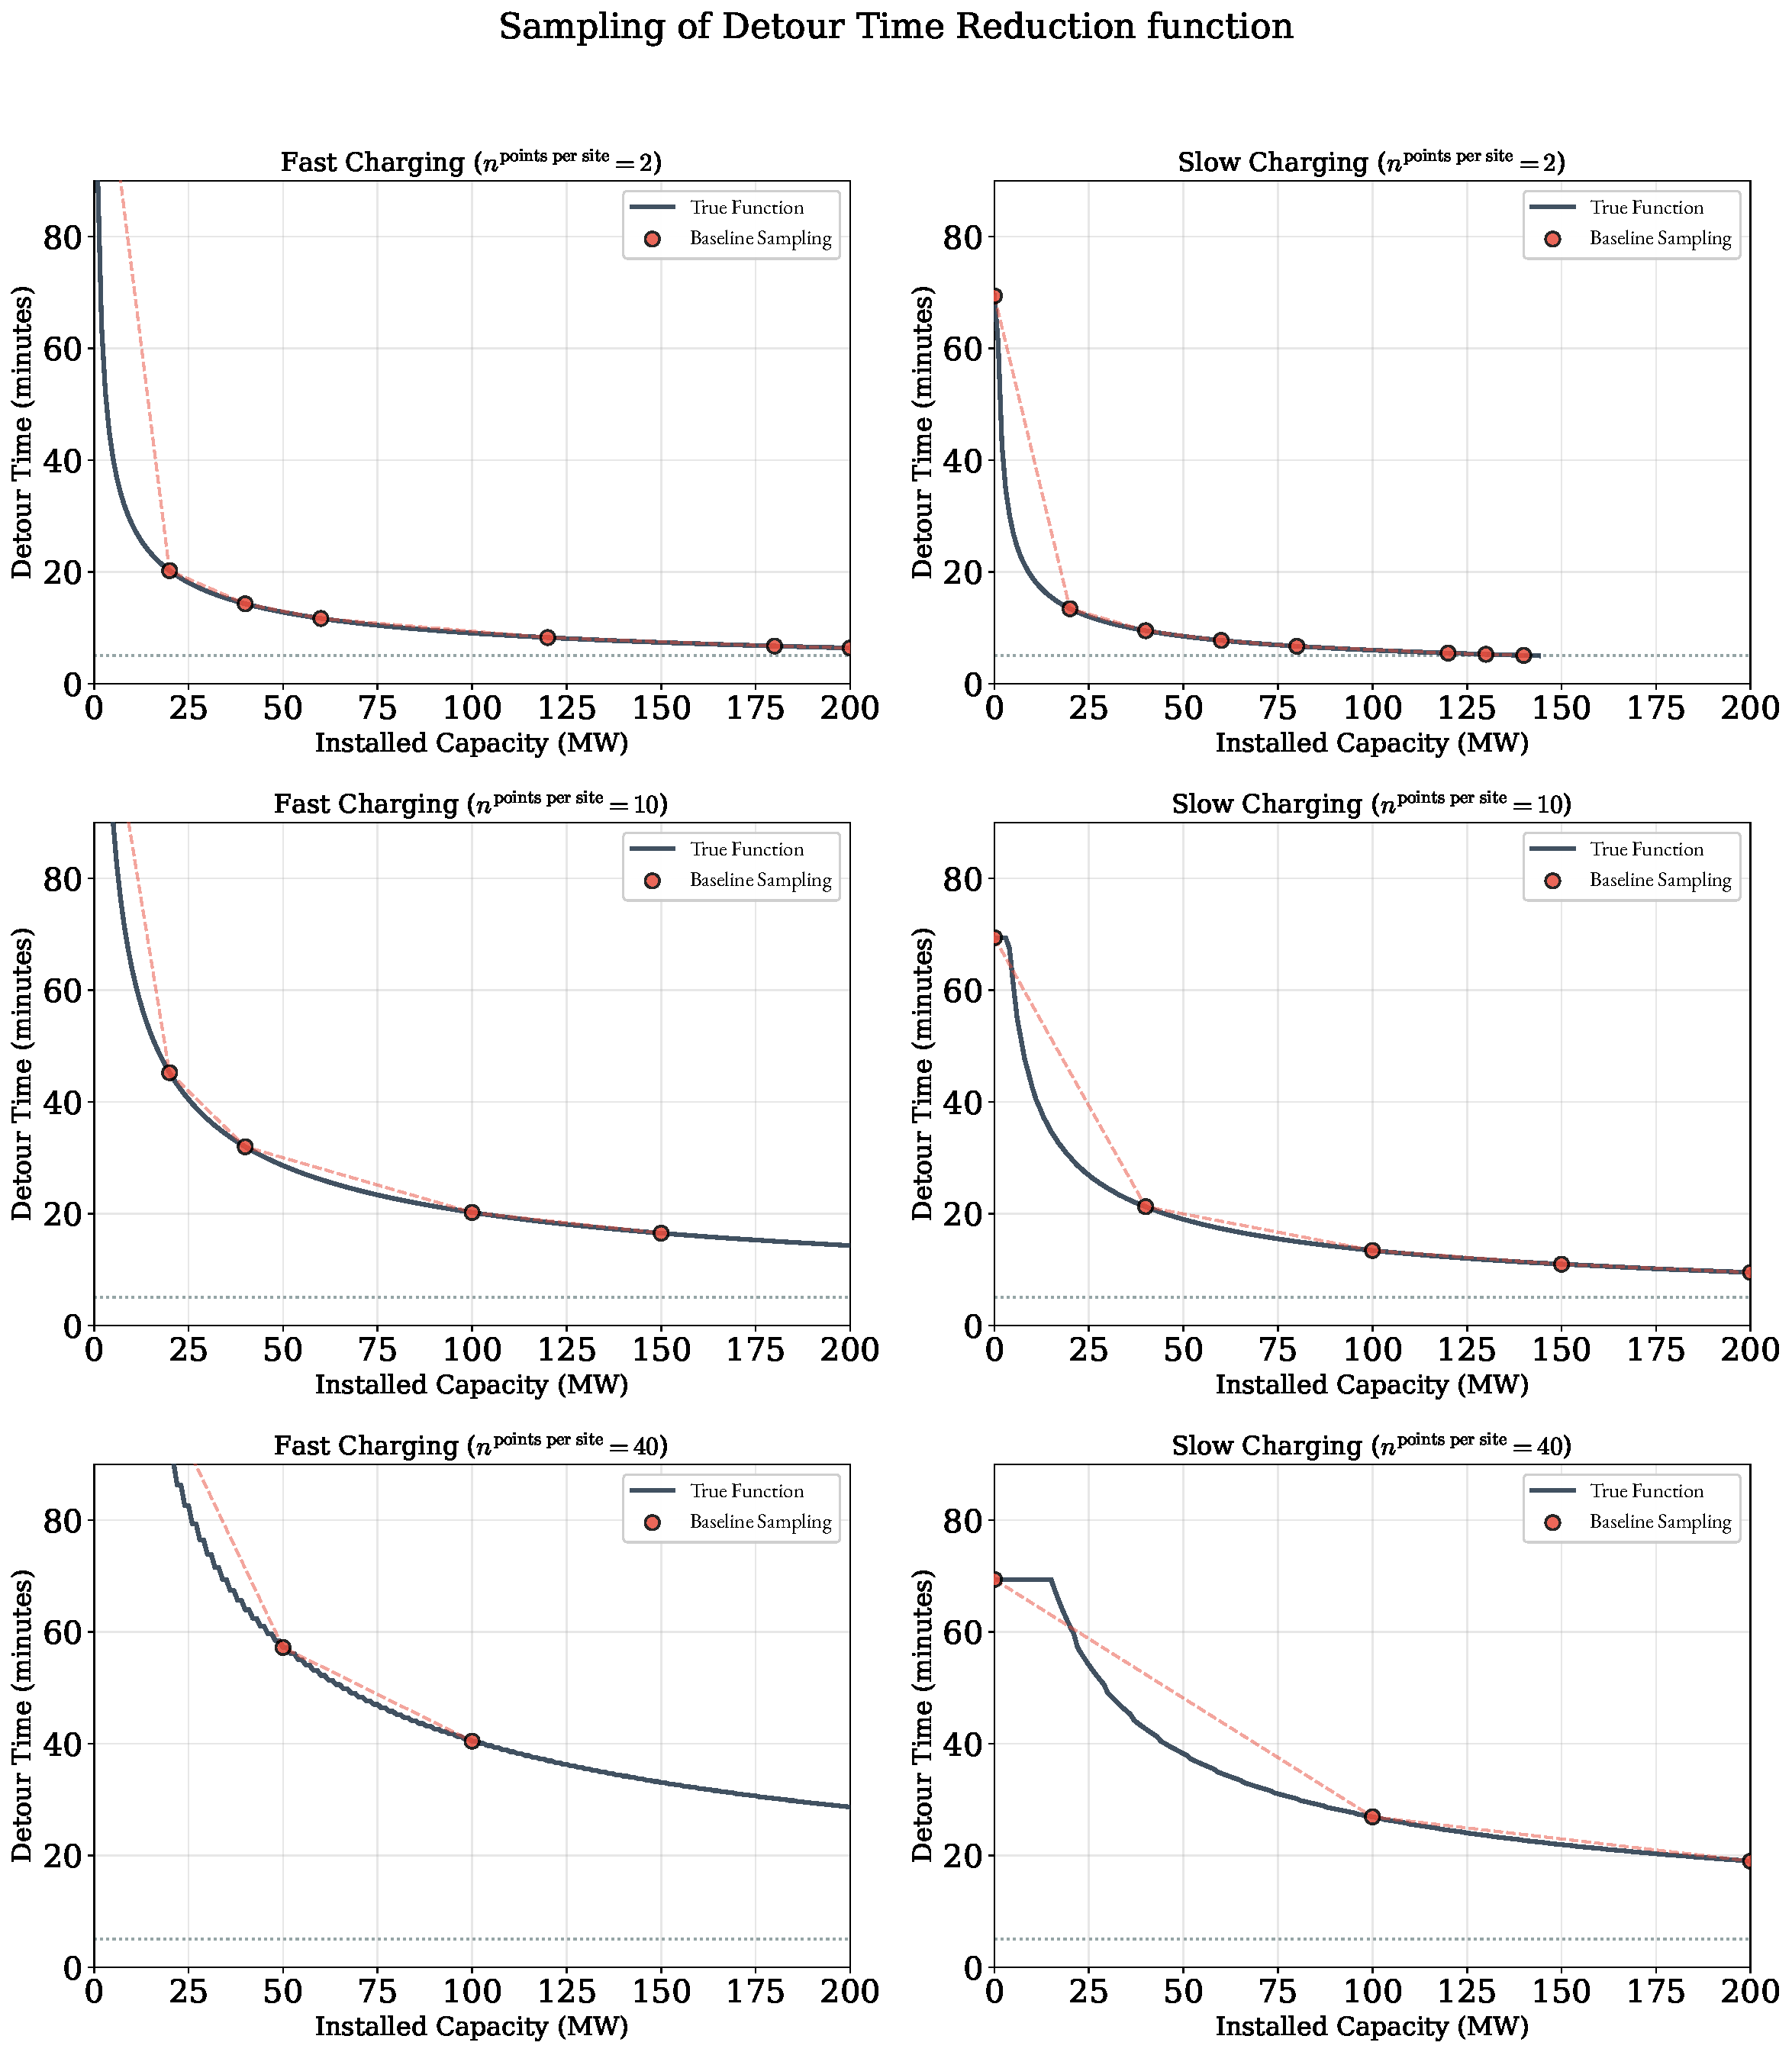
\includegraphics[width=0.9\textwidth]{graphics/dtf_sampling.pdf} 
    \caption{\added{Sampling of the detour fueling time functions to introduce the relation between charging infrastructure capacity expansion and detour fueling time to the MILP.}} \label{fig: sampling}
\end{figure} 


% \subsection{Validation}

    
% relevant parametrization for calibration are:
% \begin{itemize}
%     \item Monetary budgets by income class
%     \item Frequency of purchase
%     \item 
% \end{itemize}
% The calibration is performed to validate the stability of vehicle purchases. We model the time horizon of 20 years, including second-hand vehicle market, different vehicle sizes and that no modal shift is happening.


% To validate the data and structural assumptions of the model, we compare the magnitudes of the following parameters with existing data observations:
%     \begin{itemize}
%         \item Fleet sizing - method: comparison with todays values
%         \item Aging of fleet: validation with assumed ownership period and of function of monetary budget
%         \item Sizing of charging infrastructure: efficiency of different infrastructures; comparison with projections/ relative dimensioning via fleet size / BEV:CP ratio! 
        
%     \end{itemize}

\added{\section{Sensitivity analyses}}
\added{In this section, we present the results of sensitivity analysis conducted for four crucial features of the modeling.}

\added{\subsection{Spatial densification}} \label{sec:app_spatialdens}
\added{The function $g(q^{fuel\_infr, +})$ expresses the relation between the average detouring time and the expansion of charging infrastructure. It is introduced to express the improved level of service connected to improved accessibility to charging infrastructure. It represents this relation on NUTS-2 level and is dictated by the region's size, number of charging sites in the region, average travel speed and the factor $\mu$ representing the difference in the Euclidean distance versus the distance\deleted{ in} within the transport network (see Equations \ref{equ:df_1}, \ref{equ:df_2} and \ref{equ:df_3}). We assume an average efficiency within the road network of the region. There is extensive literature studying the efficiency of road networks and expressing this via so-called \textit{circuity} which expresses the relative factor between Euclidean distance and distance in the transport network for different modes. The recent study by \citet{COSTA2025106087} has analysed circuity of different European cities for the travel modes walking and private passenger cars. In our analysis, we assume a circuity of 1.4. Figure \ref{fig: circuity_ass} displays this assumed value together with the estimated circuity values of walking and driving for different European cities by \citet{COSTA2025106087}.}
\begin{figure}[H]
    \centering
    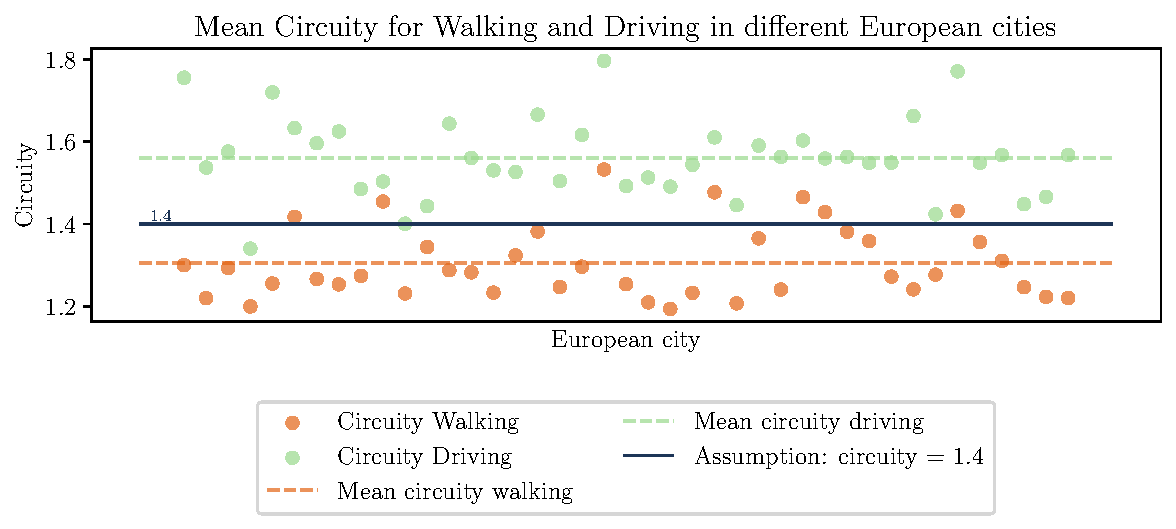
\includegraphics[width=0.7\textwidth]{graphics/mean_circuity_plot.pdf} 
    \caption{\added{Circuity values for European cities published by \citet{COSTA2025106087}}} \label{fig: circuity_ass}
\end{figure} 


\added{Looking at Figure \ref{fig: circuity_ass}, the assumed circuity $\mu = 1.4$ resembles high values for driving and low ones for walking, while detouring to the closest charging site can also include walking.}

\added{To explore the impact of this assumption, we implement the reviewer's suggestion for sensitivity analyses by varying the parameter $\mu$ according to the ranges of empirically investigated circuity. For this we test the range $\mu \in [1.0, 1.2, 1.4, 1.6, 1.8, 2.0, 2.2, 2.4]$, which we derive from reported values by \citet{COSTA2025106087}. While lower circuity reflects high efficiency of transport networks, which can be present in both rural and urban networks, high values of $\mu$ reflect lower efficiency, which can be also, for example, present in networks with many one-way roads. Studies on circuity are scarce for non-urban environments. The paper by \citet{f10121147} is an exception and studied forest roads in mountainous areas, finding an average circuity for driving at 1.55, and maximum values at up to 2.1. The resulting alternative curves for the charging infrastructure expansions are displayed in Figure \ref{fig: alternative_g_SA}. The sensitivity analysis is conducted based on one densification case, i.e., the $n^{\mathrm{points~per~site}}= 10$.}

\begin{figure}[H]
    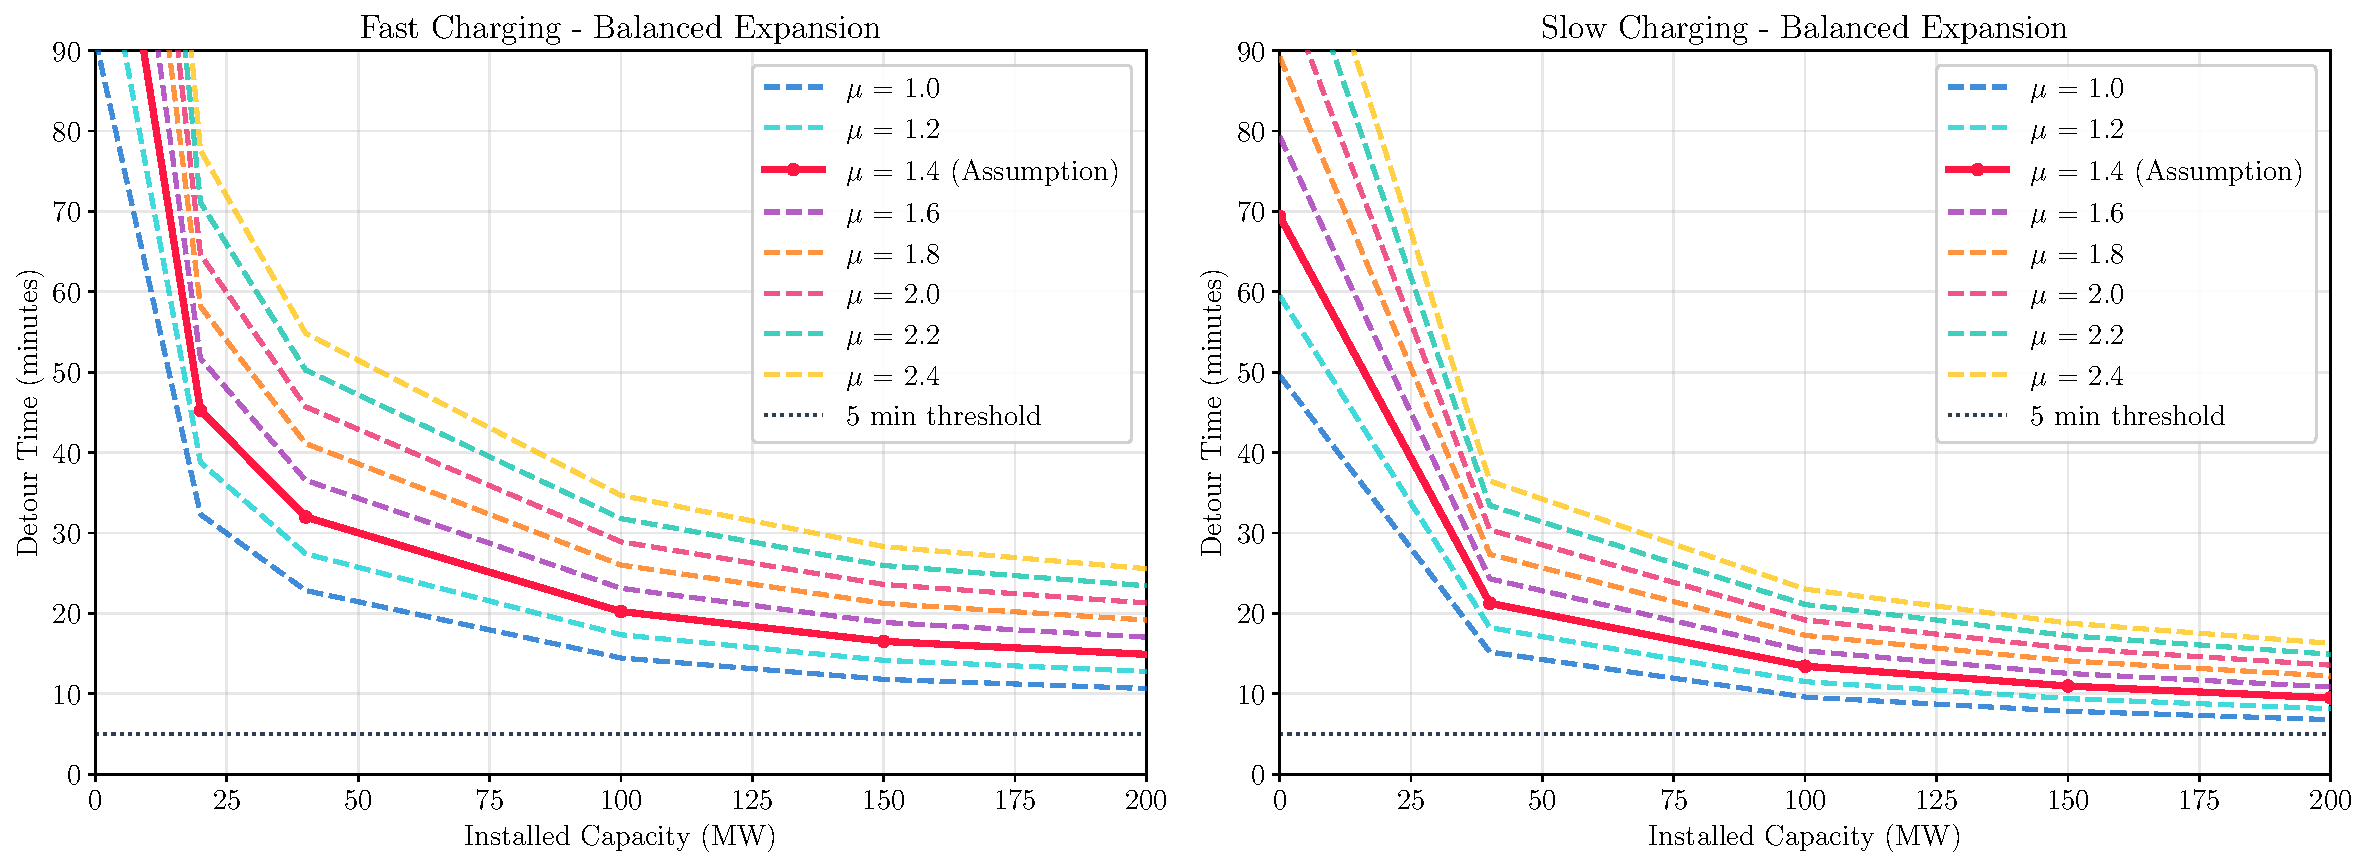
\includegraphics[width=\textwidth]{graphics/detour_time_curves_alpha_sensitivity_balanced.pdf} 
    \caption{\added{Tested curves for sensitivity analysis for different detour fueling time functions.}} \label{fig: alternative_g_SA}
\end{figure} 

\added{Results for the sensitivity analysis are displayed in Figures \ref{fig: SA_bev_adoption_g}, \ref{fig: SA_alpha_charged_energy} and \ref{fig: infr_comparison}.
Figure \ref{fig: SA_bev_adoption_g} displays the distribution of electrification shares over all tested $\mu$ values. The highest spread is visible in 2040 for the \textit{Medium low income} consumer group. Charging infrastructure utilization patterns by the different consumer groups are visible in Figure \ref{fig: SA_alpha_charged_energy}. We observe here the differences for the charging patterns for 2050. The differences among the different income classes are roughly consistent. The key observations are:}
\begin{itemize}
    \item \added{The consumer group \textit{Very low income} mostly charges using fast charging throughout all cases. An exception for this is the scenario run $\mu = 2.0$ during which the optimal solution yielded lower fast charging usage.}
    \item \added{With increasing value of the circuity $\mu$, i.e. at lower efficiency of the transport network, work place charging is also used by consumer groups of lower income classes.}
\end{itemize}

\added{Figure \ref{fig: infr_comparison} displays the total charging infrastructure expansion for two snapshots, 2035 and 2045. Overall, there is a consistency in the relative proportions of charging infrastructure investments by charger type.}

\added{Overall, the sensitivity analysis indicates that at higher efficiency of the transport network (lower values of $\mu$), denser charging infrastructure leads to higher usage of public slow charging. At higher average travel times (higher values of $\mu$), fast charger utilization increases among \textit{Low income} and \textit{Very low income} consumers. Across all tested $\mu$ values, the cross-income effects remain qualitatively consistent—lower-income groups continue to lag in adoption and rely more heavily on fast charging.}

\begin{figure}[H]
\centering

    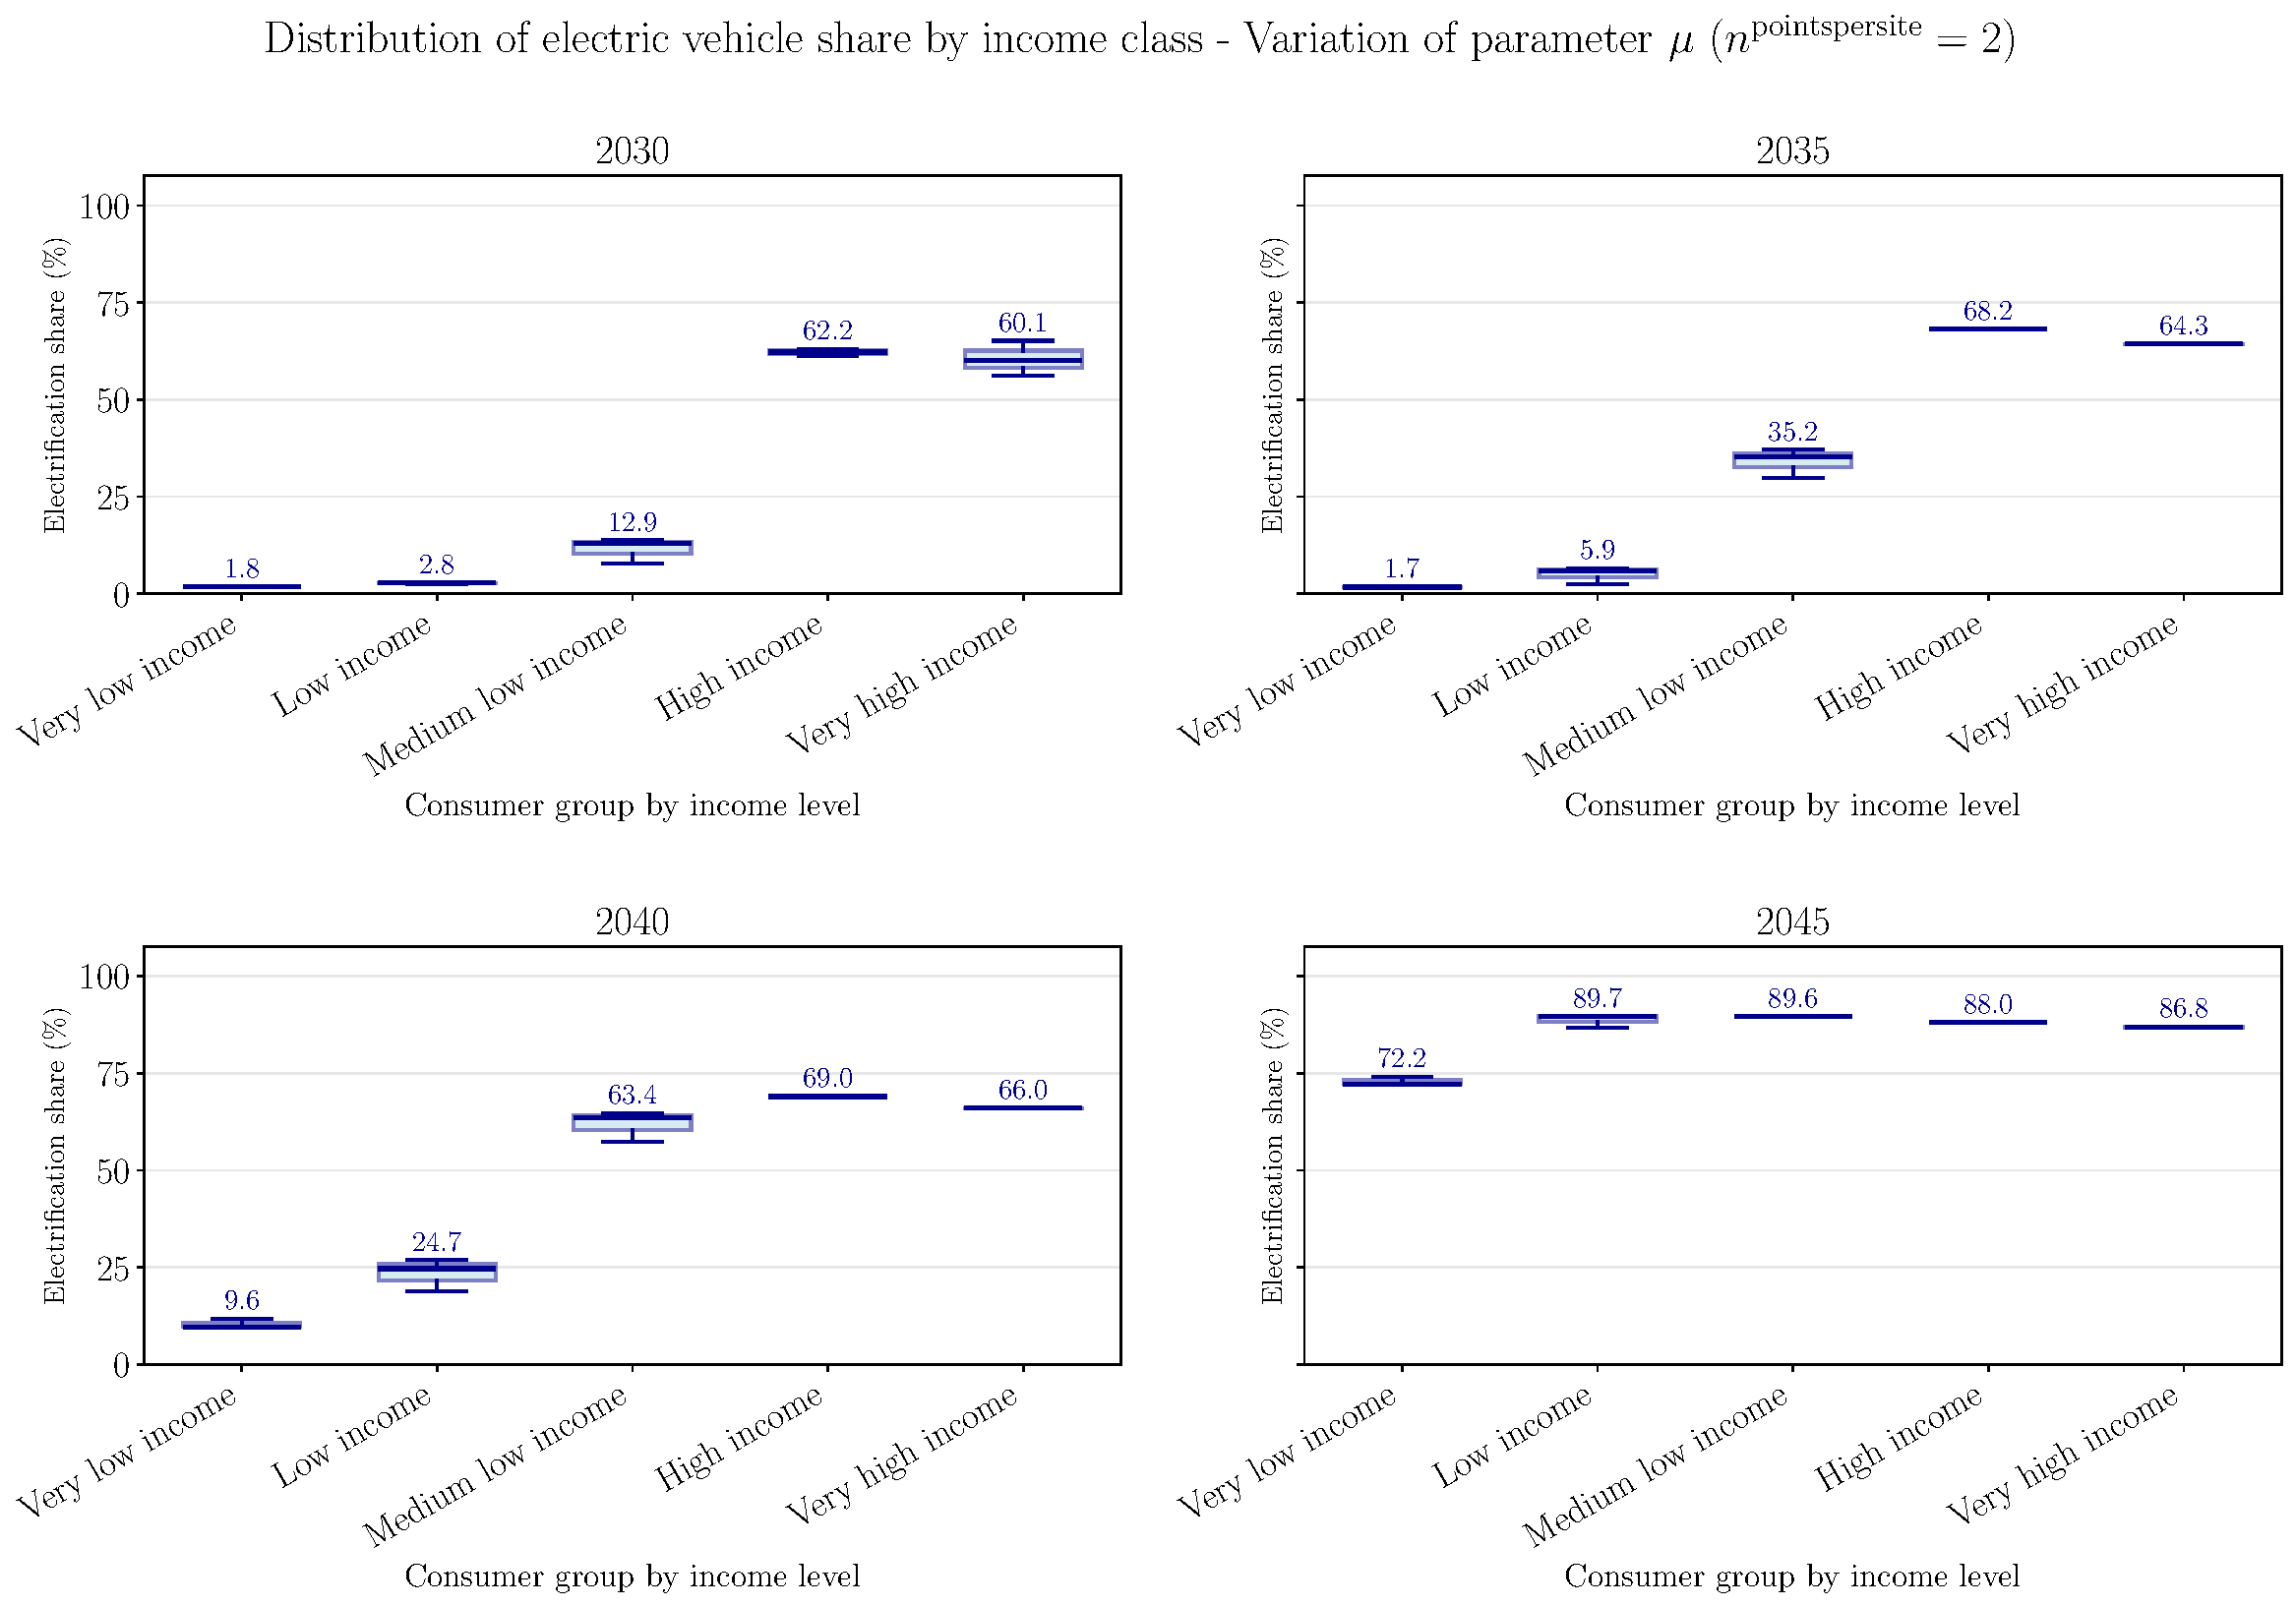
\includegraphics[width=\textwidth]{graphics/SA_alpha_boxplot_electric_vehicles_by_income.pdf} 
    \caption{\added{Distribution of development of the electrification of passenger car fleet owned by consumer groups of different income levels for different values of circuity $\mu$.}} \label{fig: SA_bev_adoption_g}
\end{figure} 


\begin{figure}[H]
\centering

    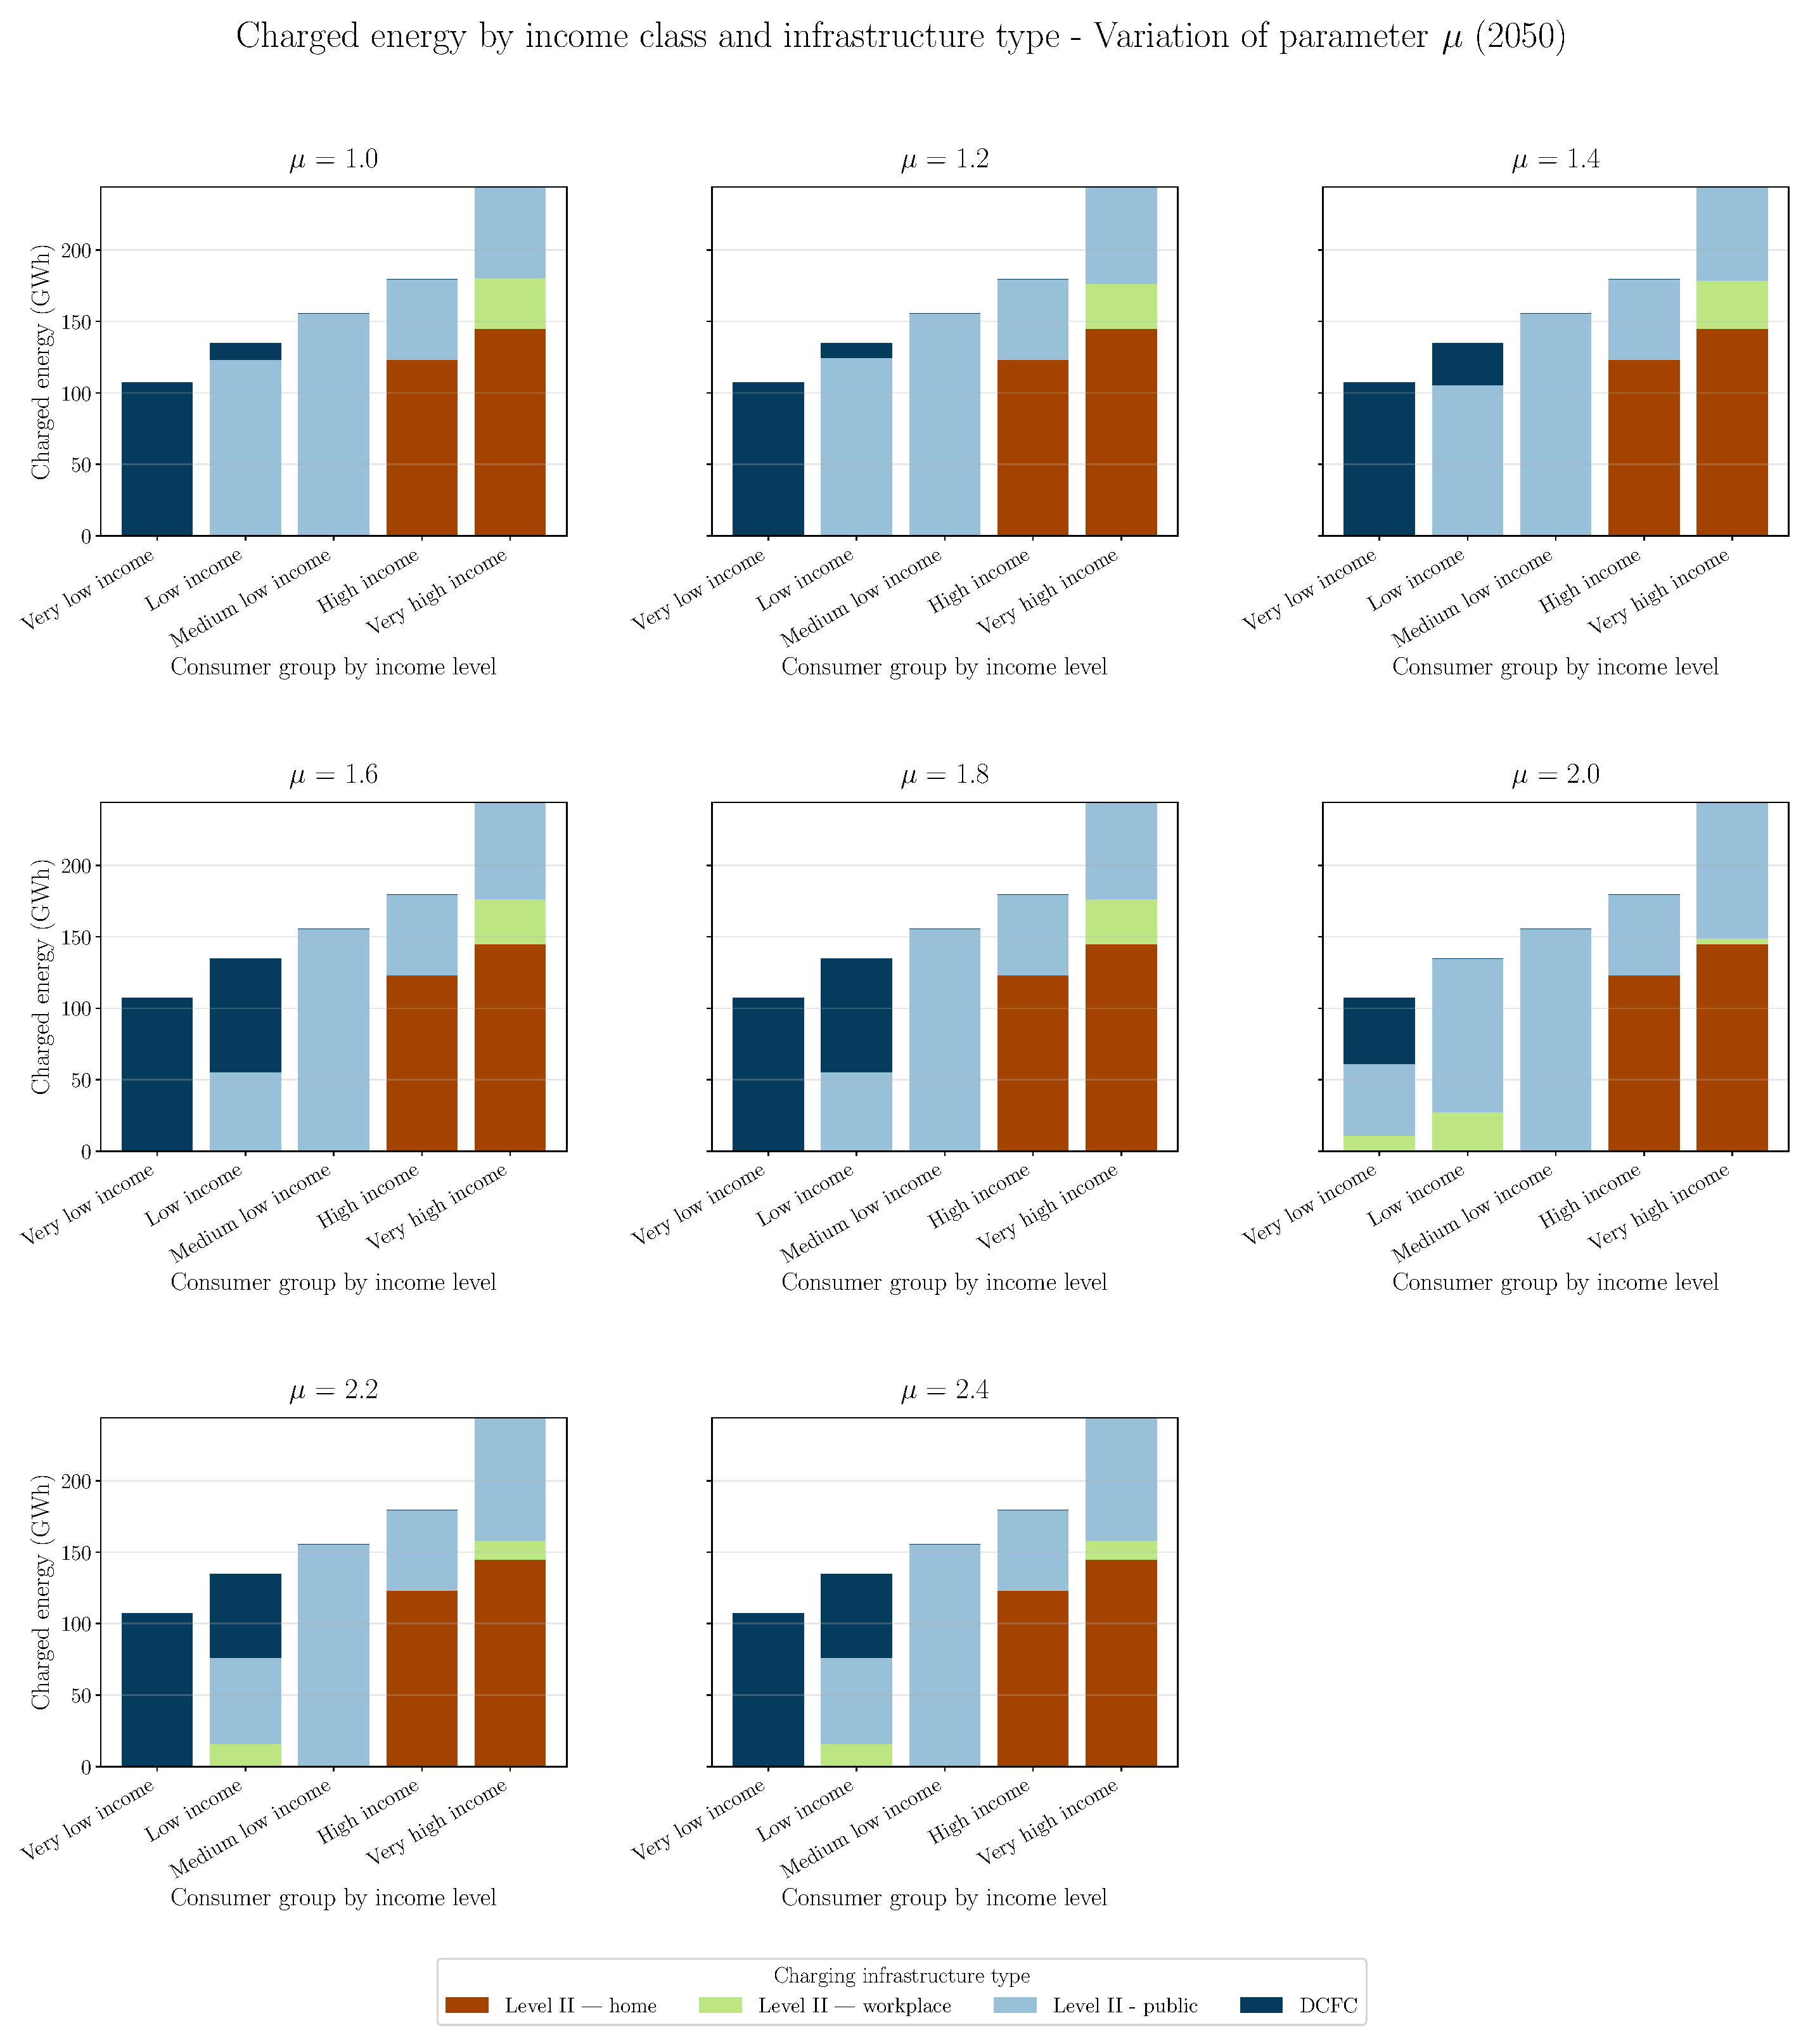
\includegraphics[width=\textwidth]{graphics/SA_alpha_charged_energy_by_income_infrastructure.pdf} 
    \caption{\added{Charger utilization in 2050 by passenger car fleet owned by consumer groups of different income levels for different values of circuity $\mu$.}} \label{fig: SA_alpha_charged_energy}
\end{figure} 



\begin{figure}[H]
\centering
    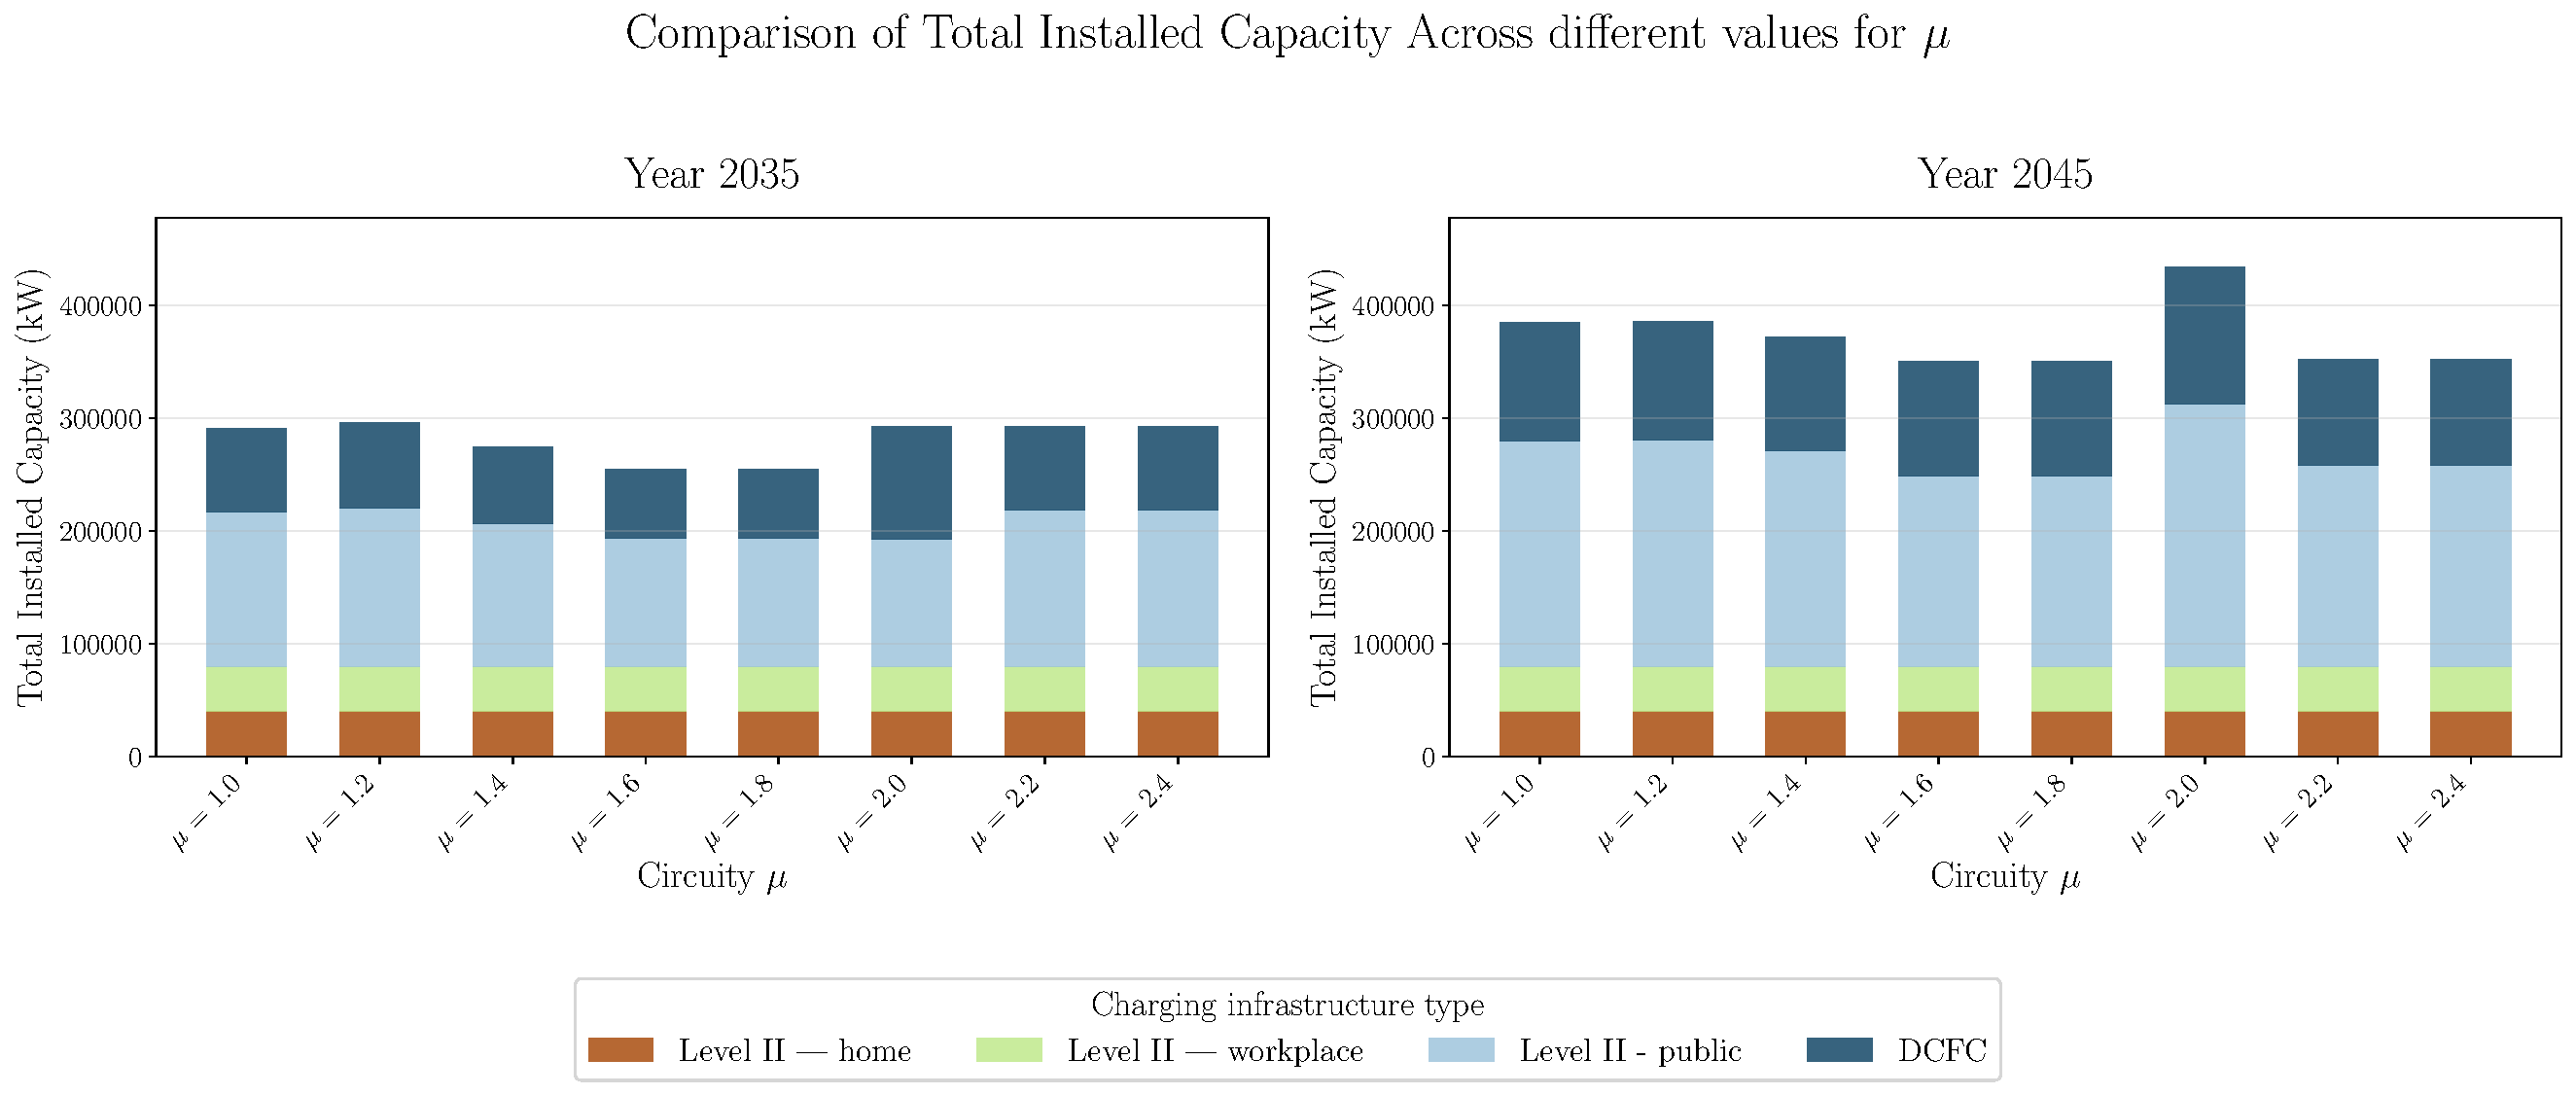
\includegraphics[width=\textwidth]{graphics/SA_alpha_capacity_comparison_2035_2045.pdf} 
    \caption{\added{Comparison for total installed charging infrastructure for different values of circuity $\mu$.}} \label{fig: infr_comparison}
\end{figure} 


\added{\subsection{Value of time}}
\added{The value of time (VoT) parameter reflects the subjective value of time for consumer groups of different income levels. We directly draw the values from \citet{TATTINI2018265} and adjust the values to the Spanish case study.}

\added{We conducted an additional sensitivity analysis to assess the potential impact of the parametrization of the VoT values. In the design of the sensitivity analysis, we tackle two aspects: Different absolute values and relative differences between the income classes. The following two figures display the tested VoT scenarios:}

\begin{figure}[H]
    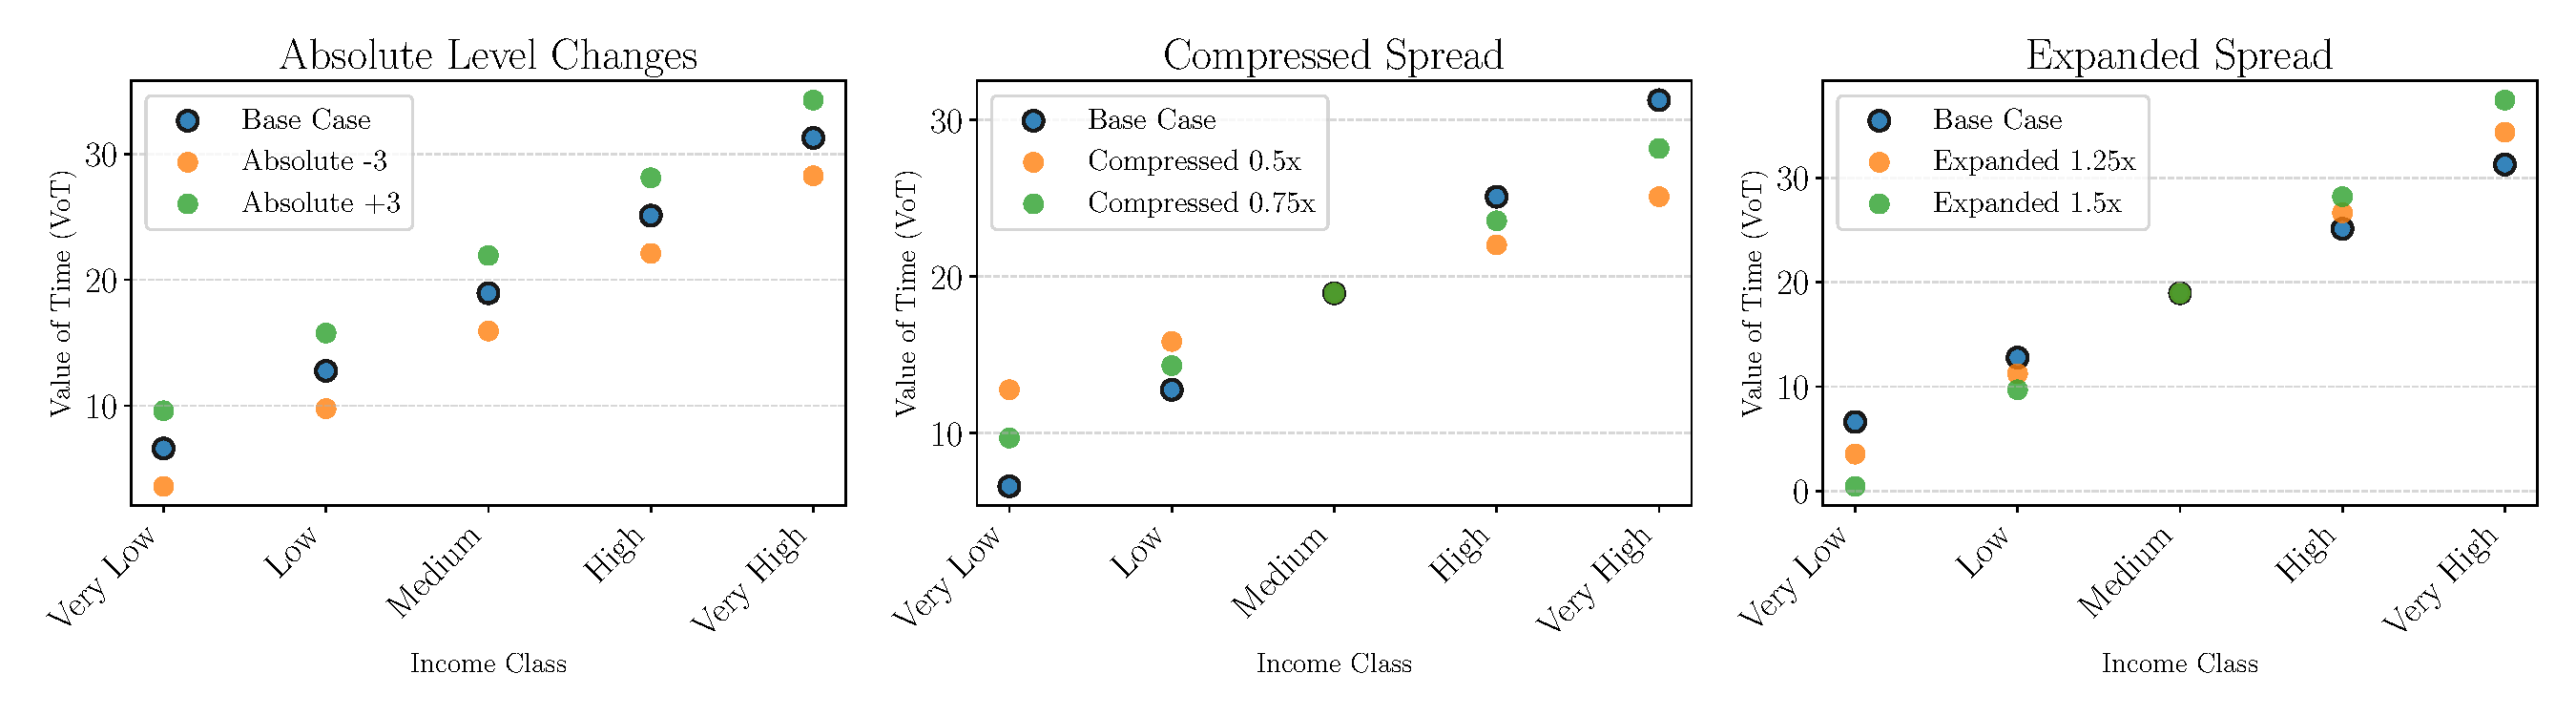
\includegraphics[width=\textwidth]{graphics/sensitivity_analysis_vot.pdf} 
    \caption{\added{The \textit{Base Case} displays the assumed VoT values for the Basque country. \textit{Left:} VoT values for absolute increase and decrease of the value of time. \textit{Center:} Two cases of smaller relative changes between the VoT per income class. \textit{Right:} Higher relative changes between the VoT per income class.}} \label{fig: VoT_tesing}
\end{figure} 

\added{The tested shifts of absolute levels are $\pm 3$ \euro/h which equal approximately absolute differences between the VoT values between inter-city vs. urban car trips in Spain \citep{WARDMAN201693}. As the \textit{Base Case} for this sensitivity analysis we use the densification scenario of $n^{\mathrm{points~per~site}} = 10$.}

\added{Figure \ref{fig: VOT_bevs} displays the distribution of electrification shares by the consumer groups for years 2030, 2035, 2040, and 2045. Overall, no significant outliers are observed. The highest impact of the VoT parameter is visible for the consumer group \textit{Medium low income}. This particularly becomes visible for the years 2035 and 2040, where the spread is up to around 45\%. The extreme values here are particularly given by \textit{Expanded 1.25x} and \textit{Expanded 1.5x}, and \textit{Compressed 0.5x} and  \textit{Compressed 0.75x}. The average VoT values of these scenarios are the same. Therefore, there is a particular sensitivity to the relative differences between the income-class-specific VoT parameters in the adoption of BEVs. }

\begin{figure}[H]
    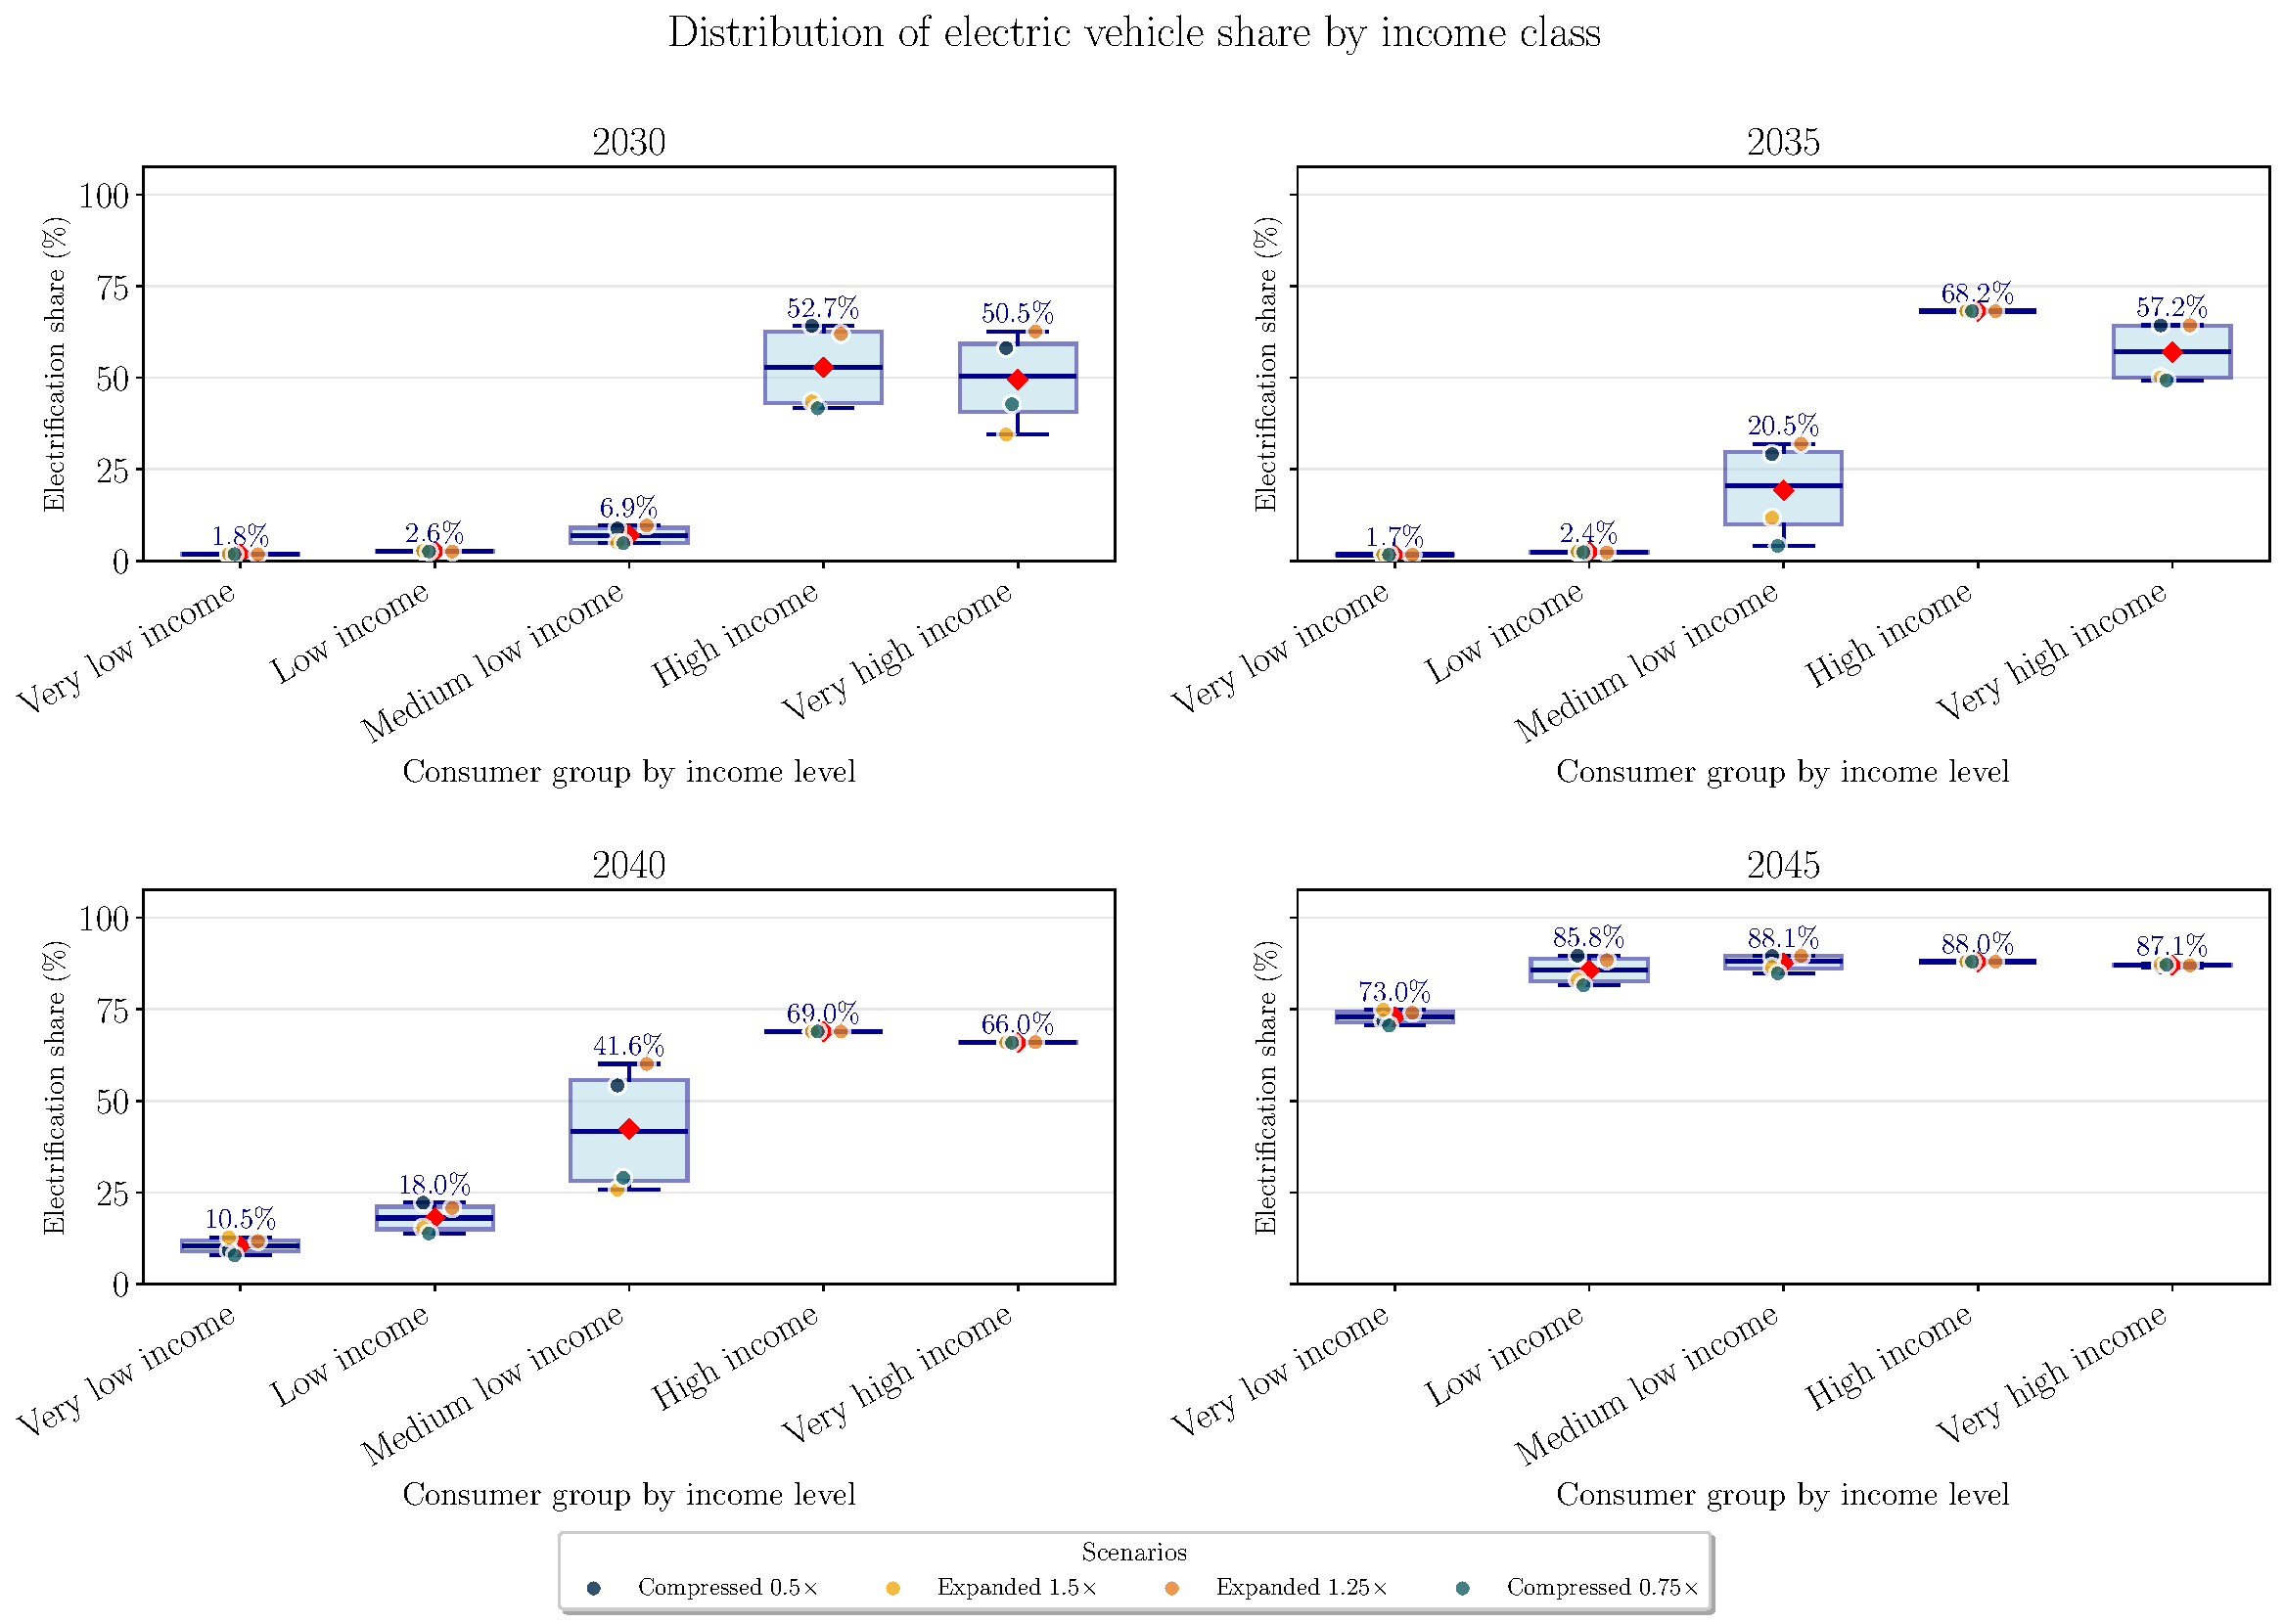
\includegraphics[width=\textwidth]{graphics/SA_boxplot_electric_vehicles_by_income.pdf} 
    \caption{\added{Distribution of the development of electrification of passenger car fleet owned by consumer groups of different income levels observed during sensitivity analysis of different VoT scenarios.}} \label{fig: VOT_bevs}
\end{figure} 

\added{We next examine the differences in charged energy across charger types (see Figure \ref{fig: VOT_charging_pat}). We show a snapshot for 2050 displaying the usage patterns by the 100\% electrified fleet for a selection of four different VoT scenarios. While there are no significant changes for consumer groups \textit{Very high income}, \textit{High income}, and \textit{Medium low income}, the amount of fast charging capacity being used by \textit{Very low income} and \textit{Low income} varies significantly between the VoT settings.}

\added{In Figure \ref{fig: VoT_fastcharg}, we take a closer look at the usage of fast charging capacities by  \textit{Very low income} and \textit{Low income} consumer groups. In the cases where these groups have higher VoT, i.e. the VoT scenarios of \textit{Compressed 0.5x},  \textit{Compressed 0.75x} and \textit{Absolute +3}, the amount of fast charging is zero for the \textit{Low income} class.}

\begin{figure}[H]
\centering

    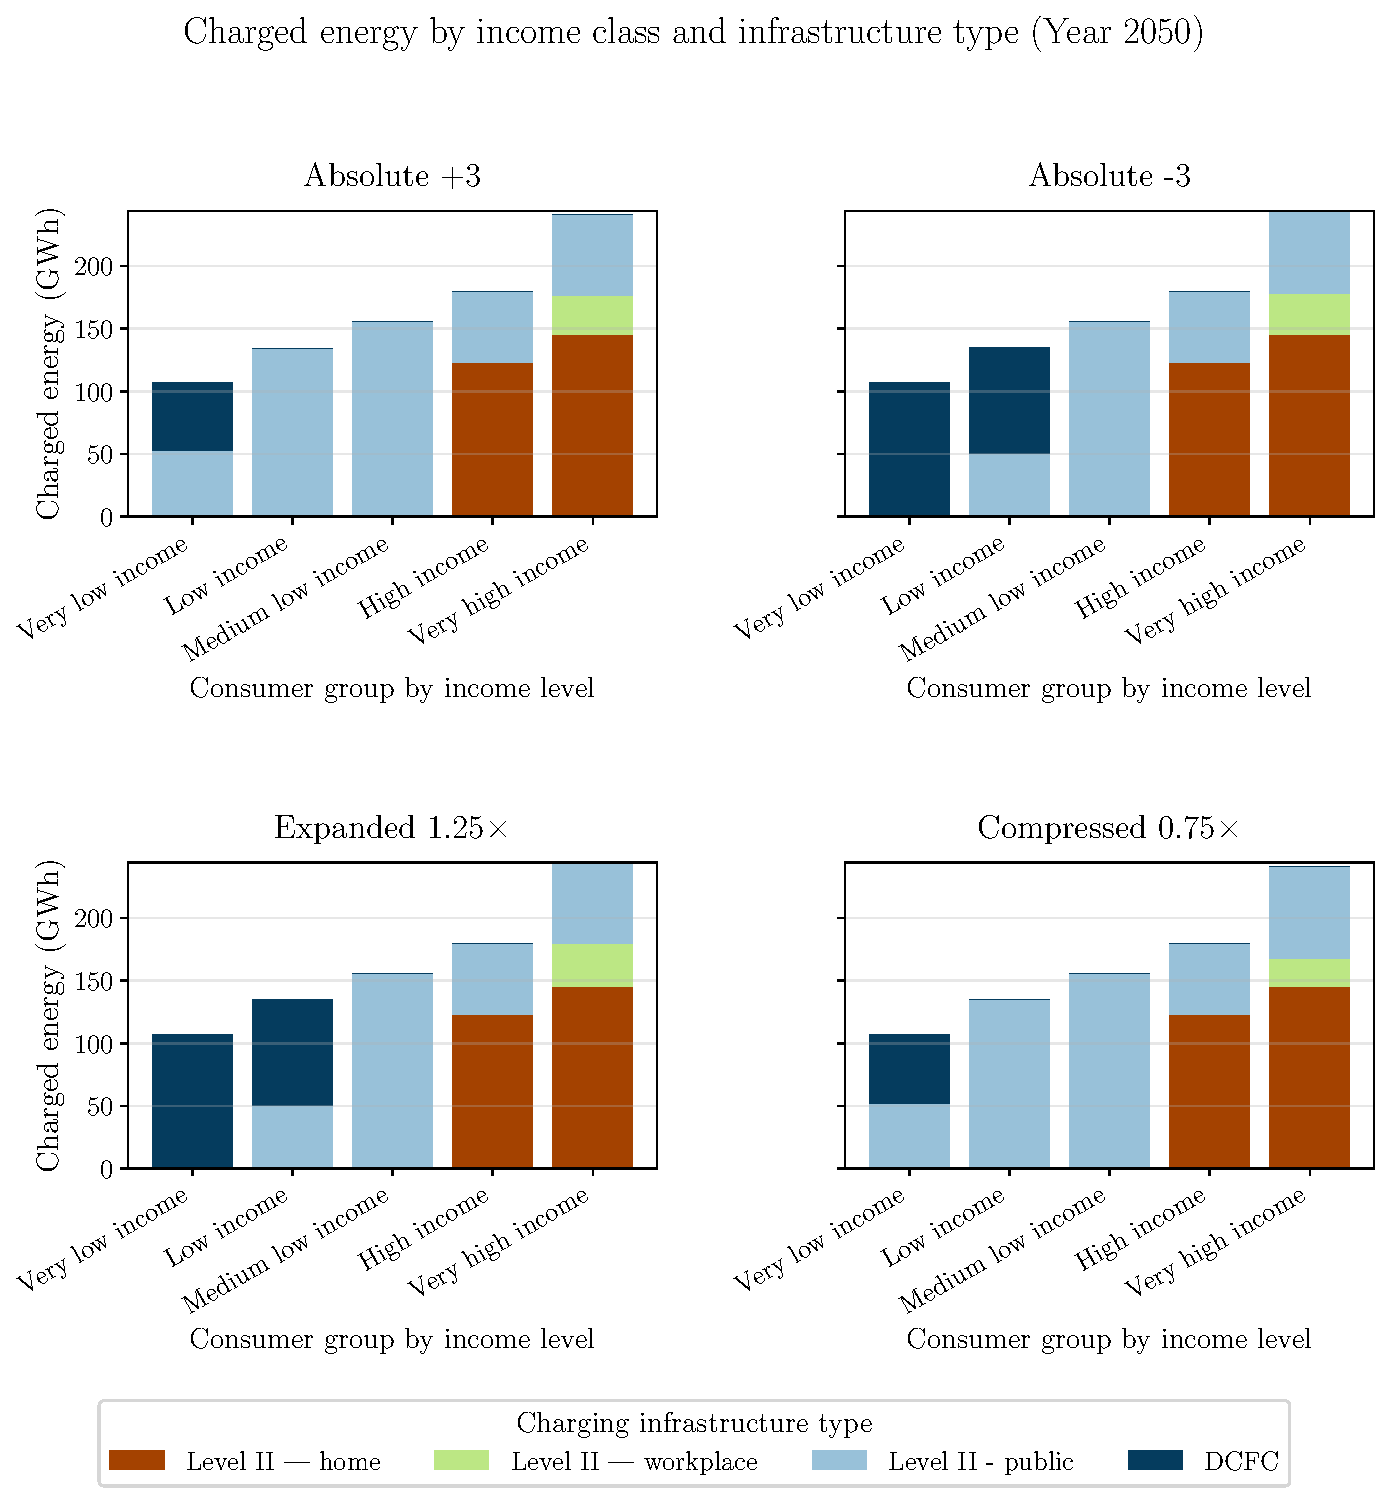
\includegraphics[width=\textwidth]{graphics/SA_charged_energy_by_income_infrastructure.pdf} 
    \caption{\added{Charged energy by charger type in 2050 for different VoT scenarios.}} \label{fig: VOT_charging_pat}
\end{figure} 

\begin{figure}[H]
\centering

    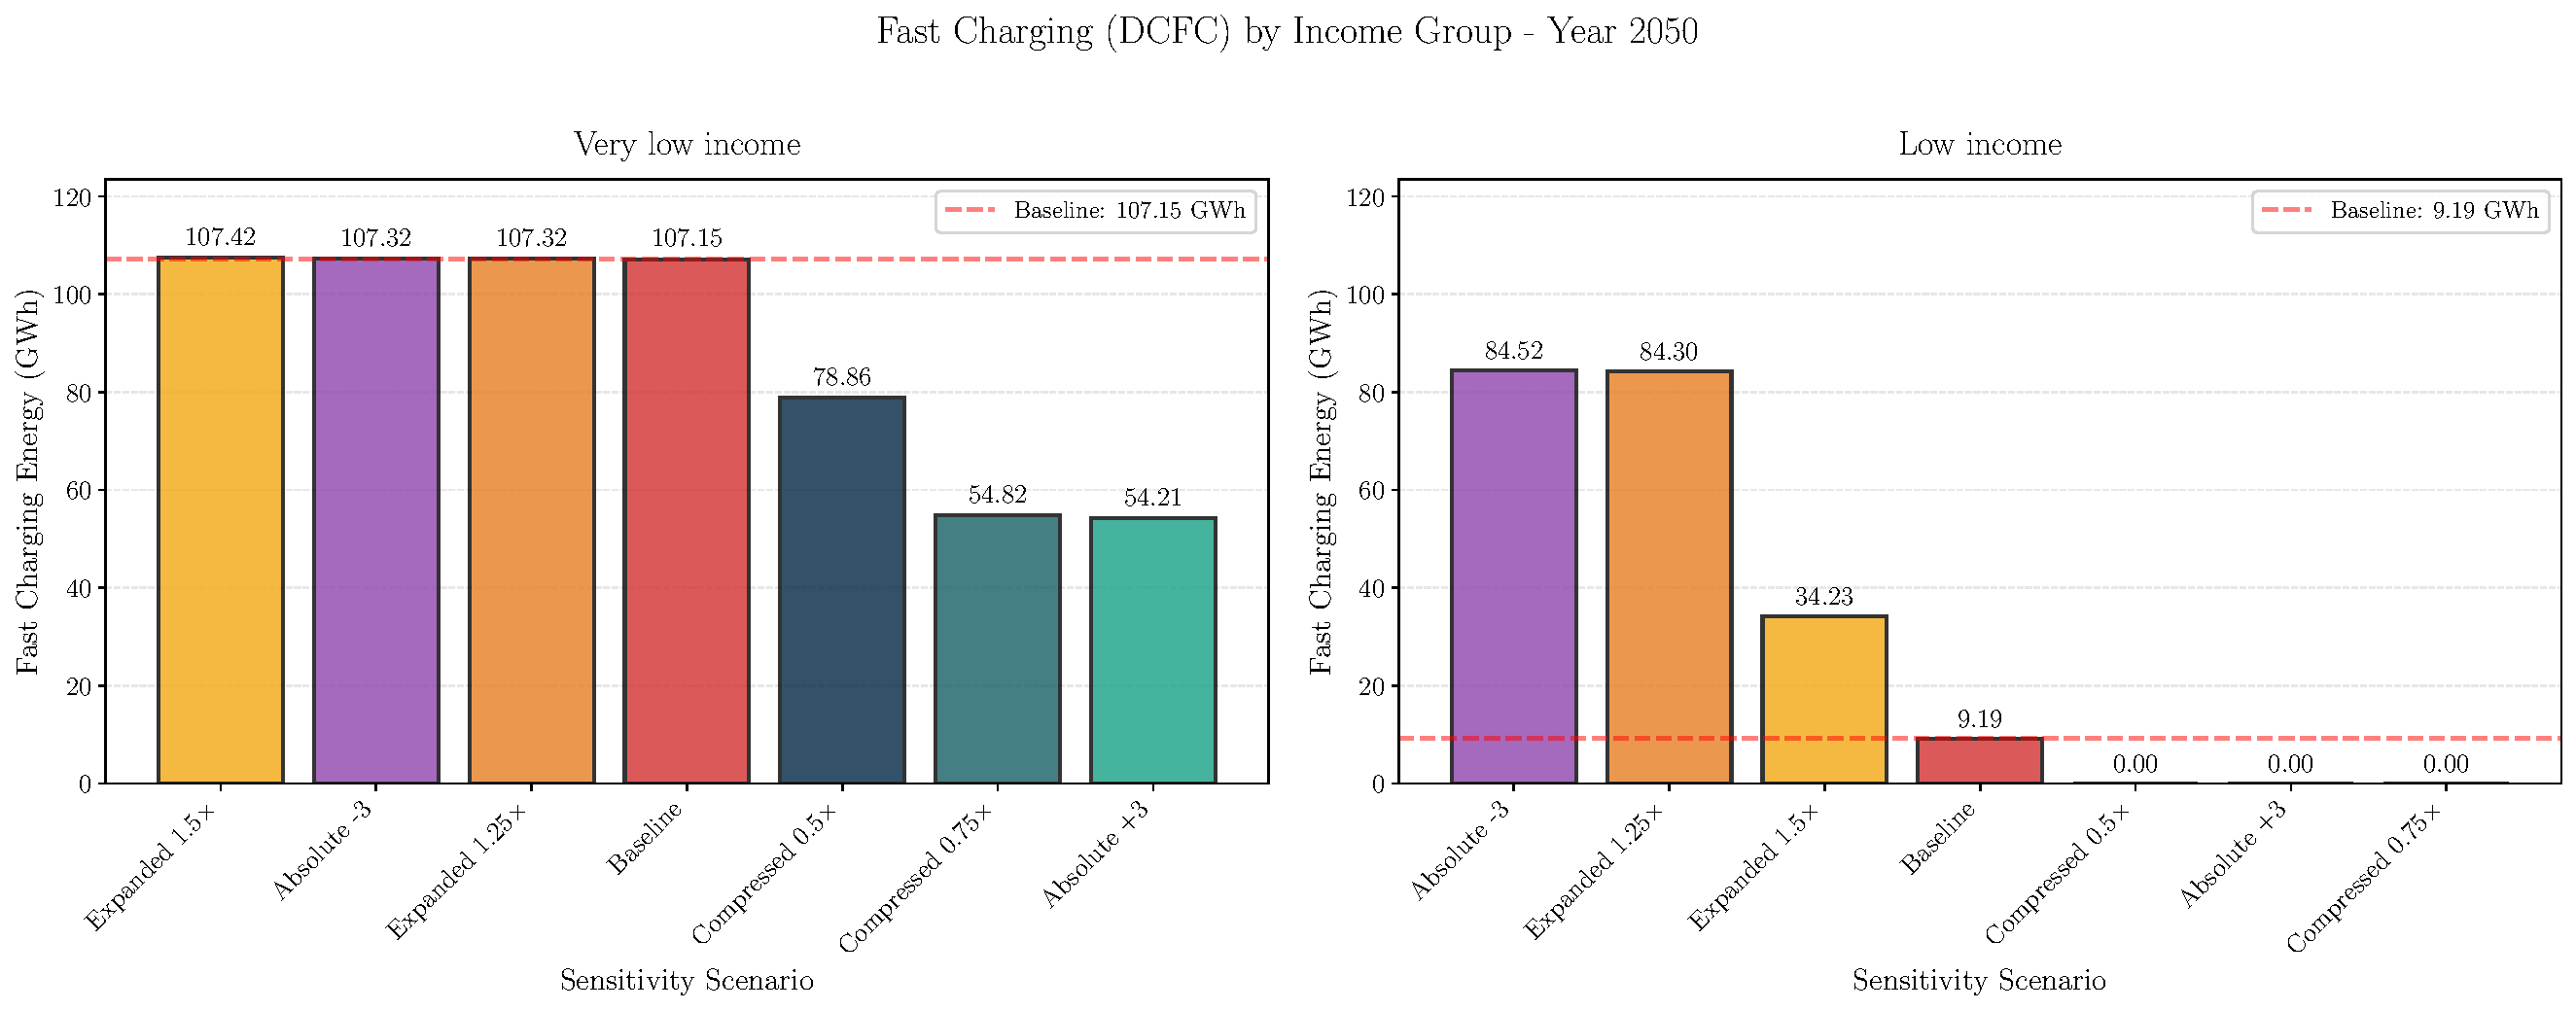
\includegraphics[width=\textwidth]{graphics/SA_fast_charging_low_income_comparison.pdf} 
    \caption{\added{Charged energy at fast chargers by consumer groups \textit{Very low income} and \textit{Low income} in 2050 for different VoT scenarios.}} \label{fig: VoT_fastcharg}
\end{figure} 

\added{This observation is consistent with observations presented in the \textit{Results} section, in particular, Section 4.1, where we show differences in fast charger utilization through variations in levels of service induced by charging infrastructure densification. There, as well as in these VoT scenarios, we observe how the term $\mathrm{VoT} \times \mathrm{level~of~service}$ influences charger-type utilization across income groups.} 


% \added{\subsection{Home charger capacities}}

% In the results presented in Section \ref{sec:res}, we observe that home charging capacities are not expanded beyond its initital availability. In the sensitivity analysis presented in the following, we impose exogeneously defined charging capacities for home charging to observe the adoption of battery-electric passenger cars and charging patterns by income classes at different scenarios of home charging capacity. 

% or this, we model expansions scenarios for home charging capacities. Based on the home ownership rates, as suggested in the comment, and number of maximum possible installation for home chargers, we determine maximum total capacities for each income class. Based on these, we draw linear expansion pathways.

% Figure \ref{fig: home_charging_exp_scenarios} displays the assumed home charging capacity expansions. The percentage value (20 - 100) represents the share of the maximum home charging capacities reached by 2050 and the pathways follow a linear development. We use here, again, the $n^{\mathrm{points per site}} = 10$ as the base scenario for the sensitivity analysis.

% \begin{figure}[H]
% \centering

%     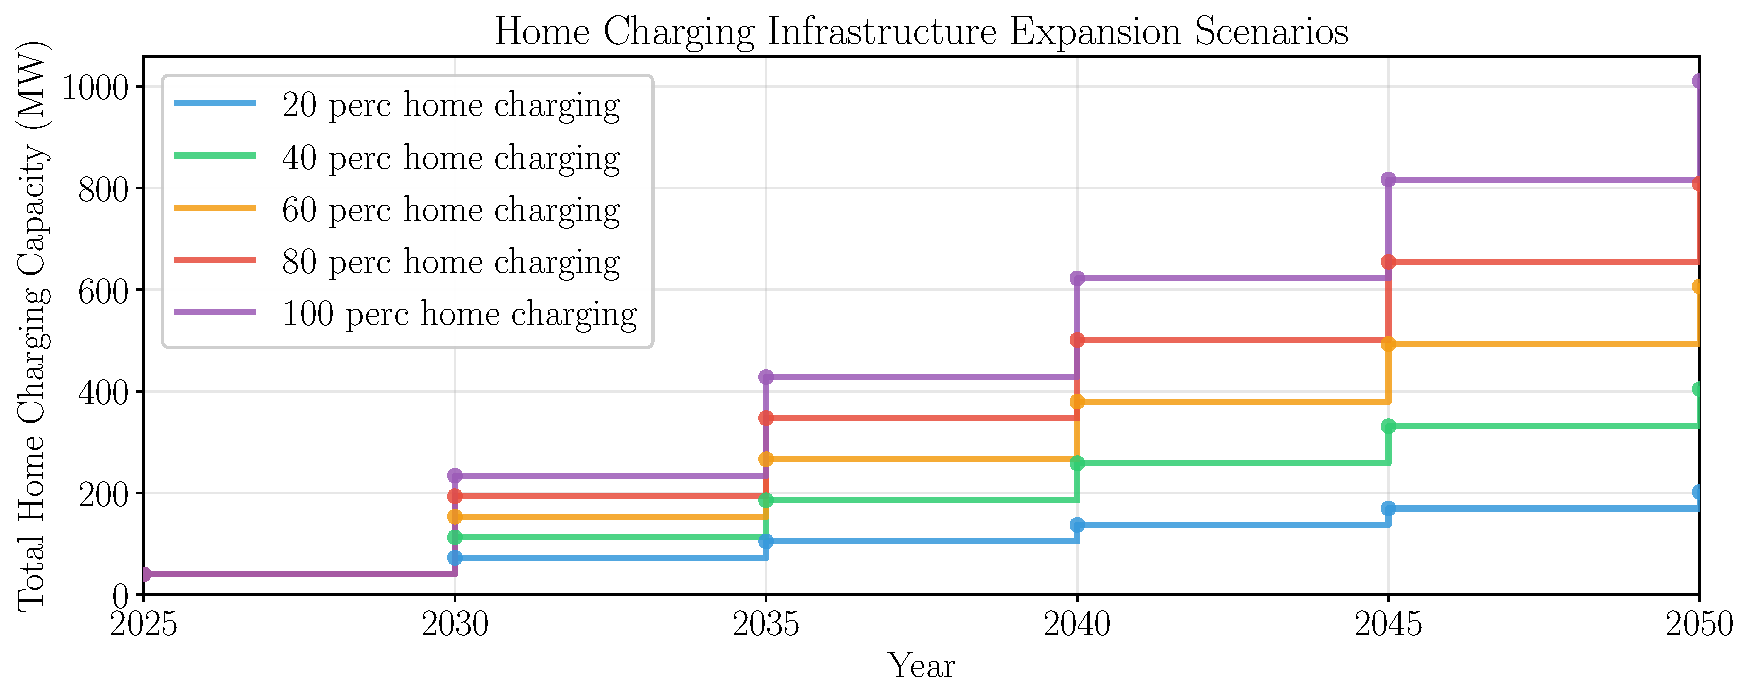
\includegraphics[width=0.9\textwidth]{graphics/home_charging_expansion_scenarios.pdf} 
%     \caption{Scenarios for expansion of home charging (exogenous).} \label{fig: home_charging_exp_scenarios}
% \end{figure} 

% Figure \ref{fig: SA_comp_cons} displays the impact of increased home charging capacities on the utilization of public charging infrastructure. The increased amount of home charger capacity shifts the charging utilization increasingly to home charging. With this, public charging plays a decreasing role in demand coverage. Though, there is no clear patterns visible in the reduction of fast charger utilization. Figure \ref{fig: SA_comp_final} shows capacity installations by charger type for two different years: 2035 and 2045. The increasing home charging capacity is clearly visible. Further, we see that in the case of no fast charger utilization (scenarios \textbf{20 perc home charging} and \textit{80 perc home charging}), the public charger capacities are expanded increasingly. 

% The unclear trend of fast charging utilization is most likely to stem from low differences between the objective function values between fast charger usage versus without fast charger usage. 

% \begin{figure}[H]
% \centering

%     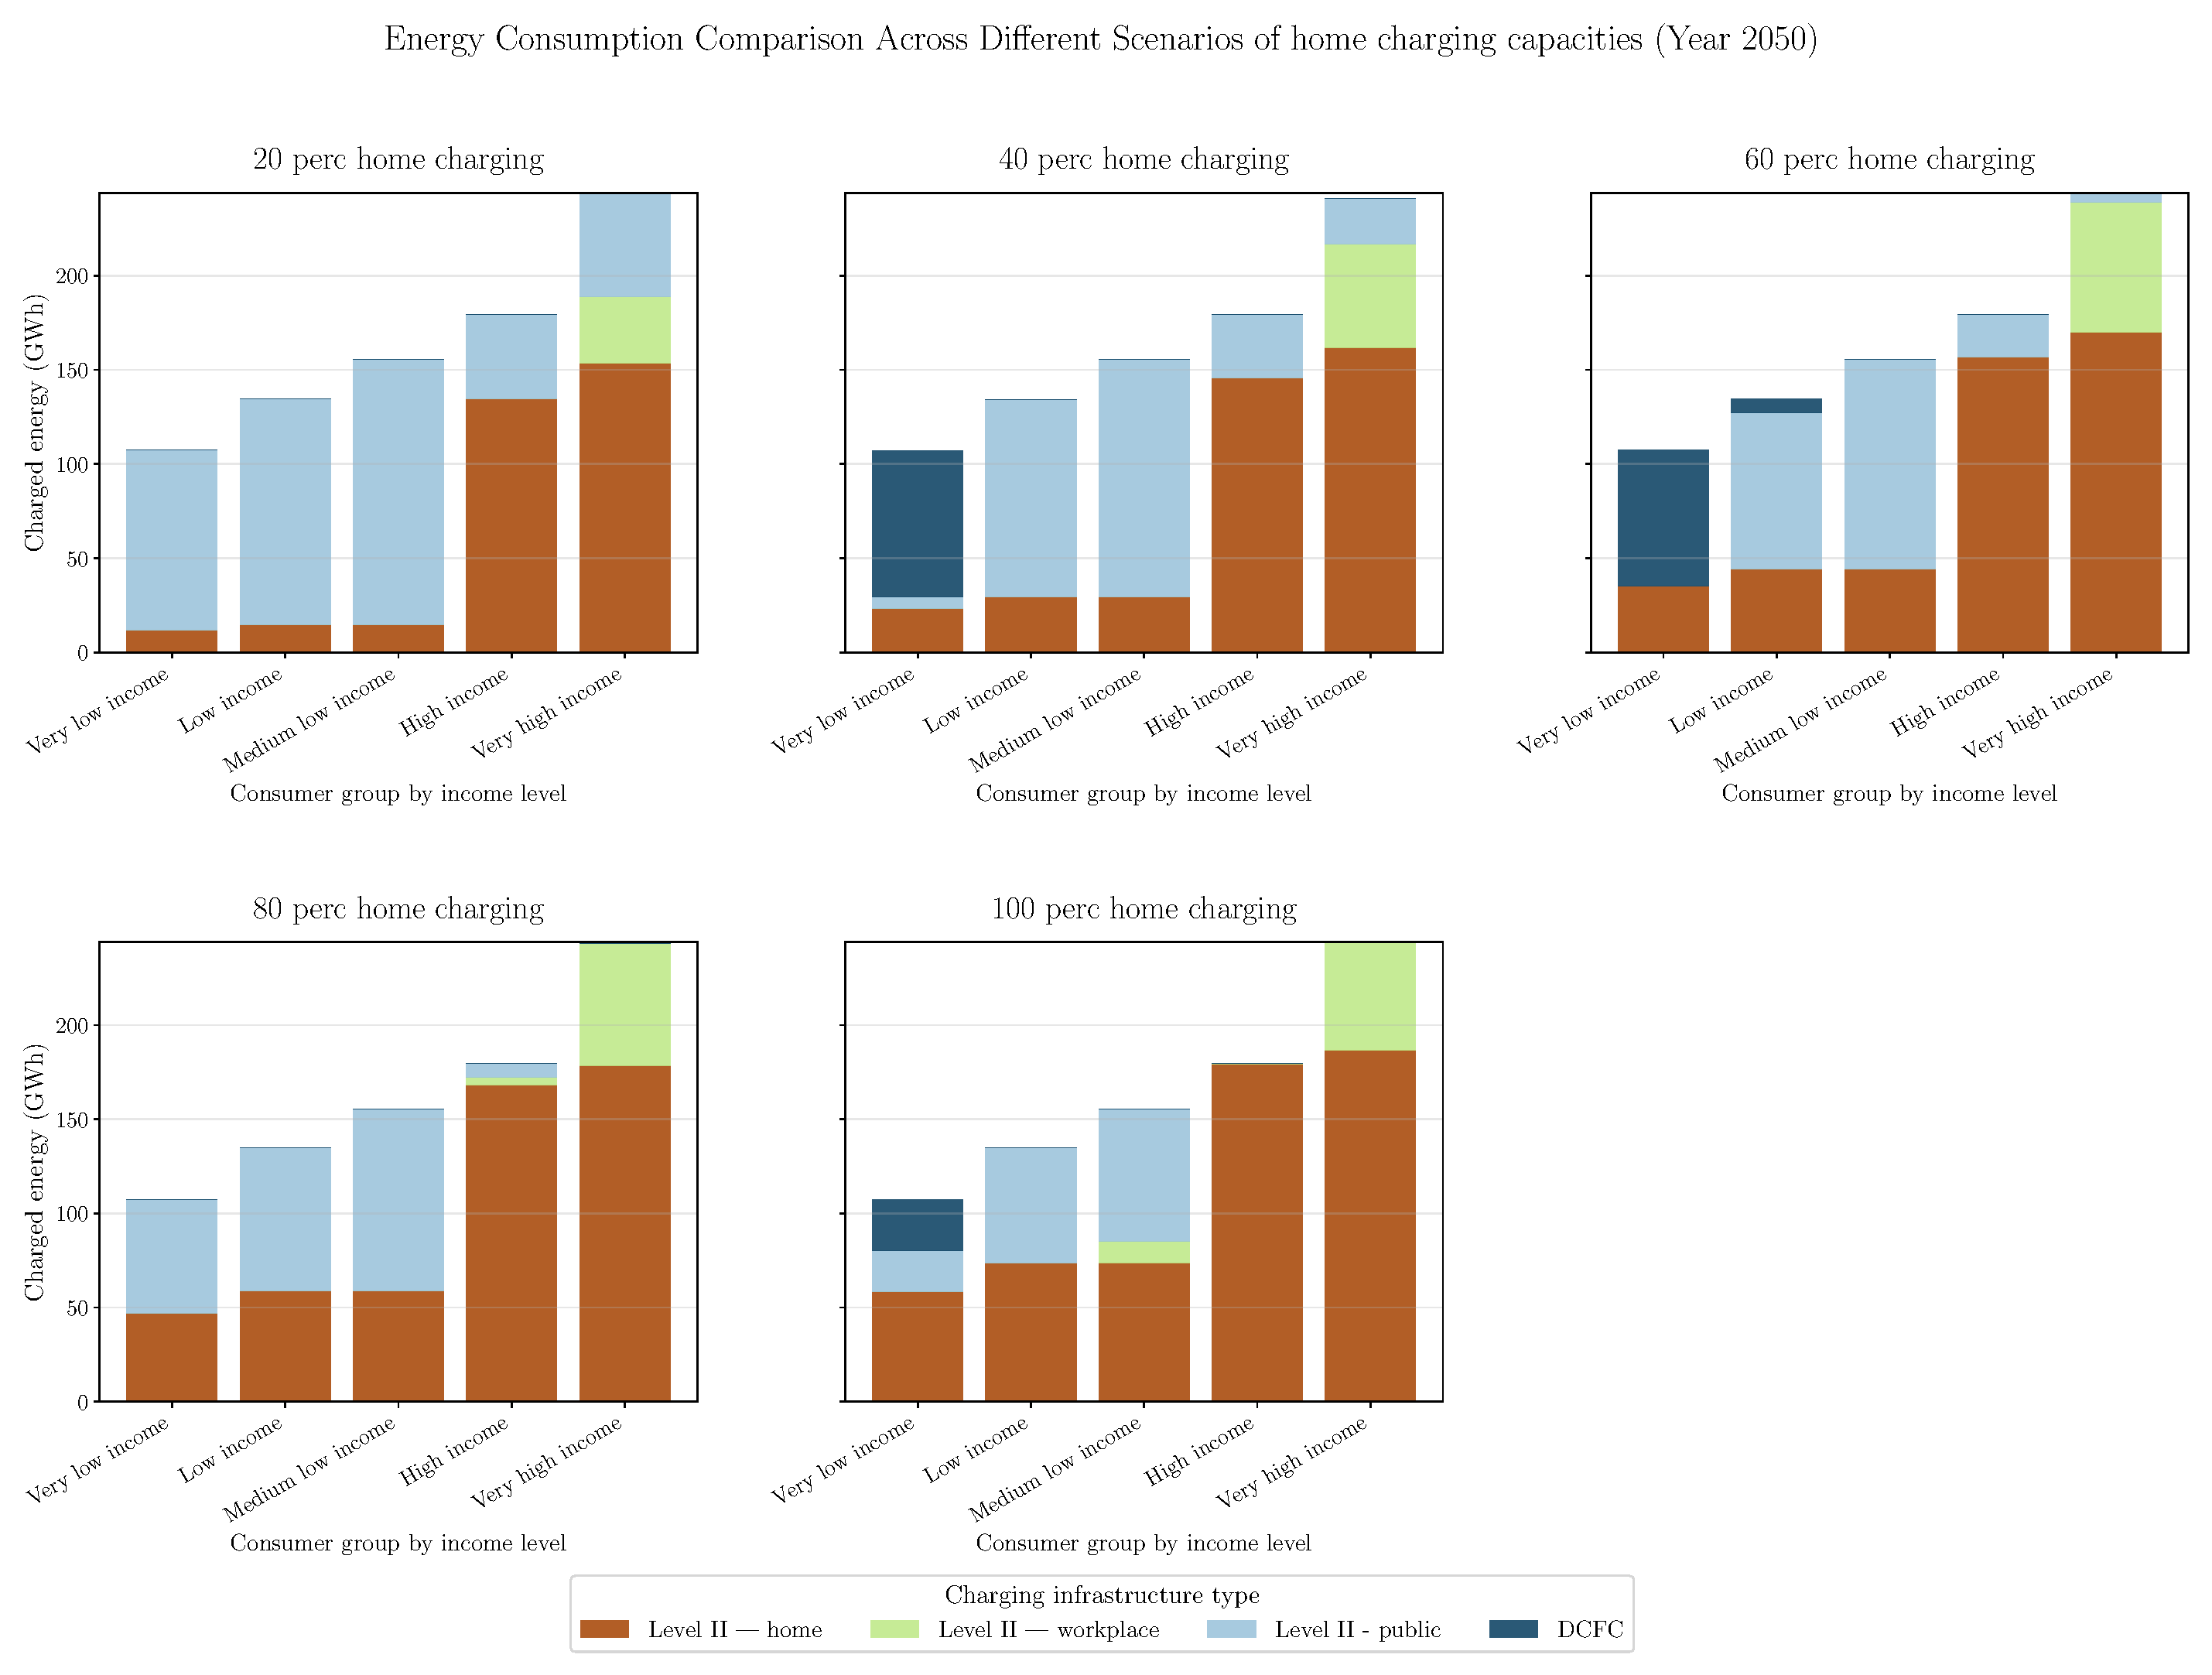
\includegraphics[width=0.9\textwidth]{graphics/SA_comparison_energy_consumption.pdf} 
%     \caption{Comparison of energy consumption patterns across income classes for different cases of exogenously defined home charging capacities.} \label{fig: SA_comp_cons}
% \end{figure} 

% \begin{figure}[H]

% \centering

%     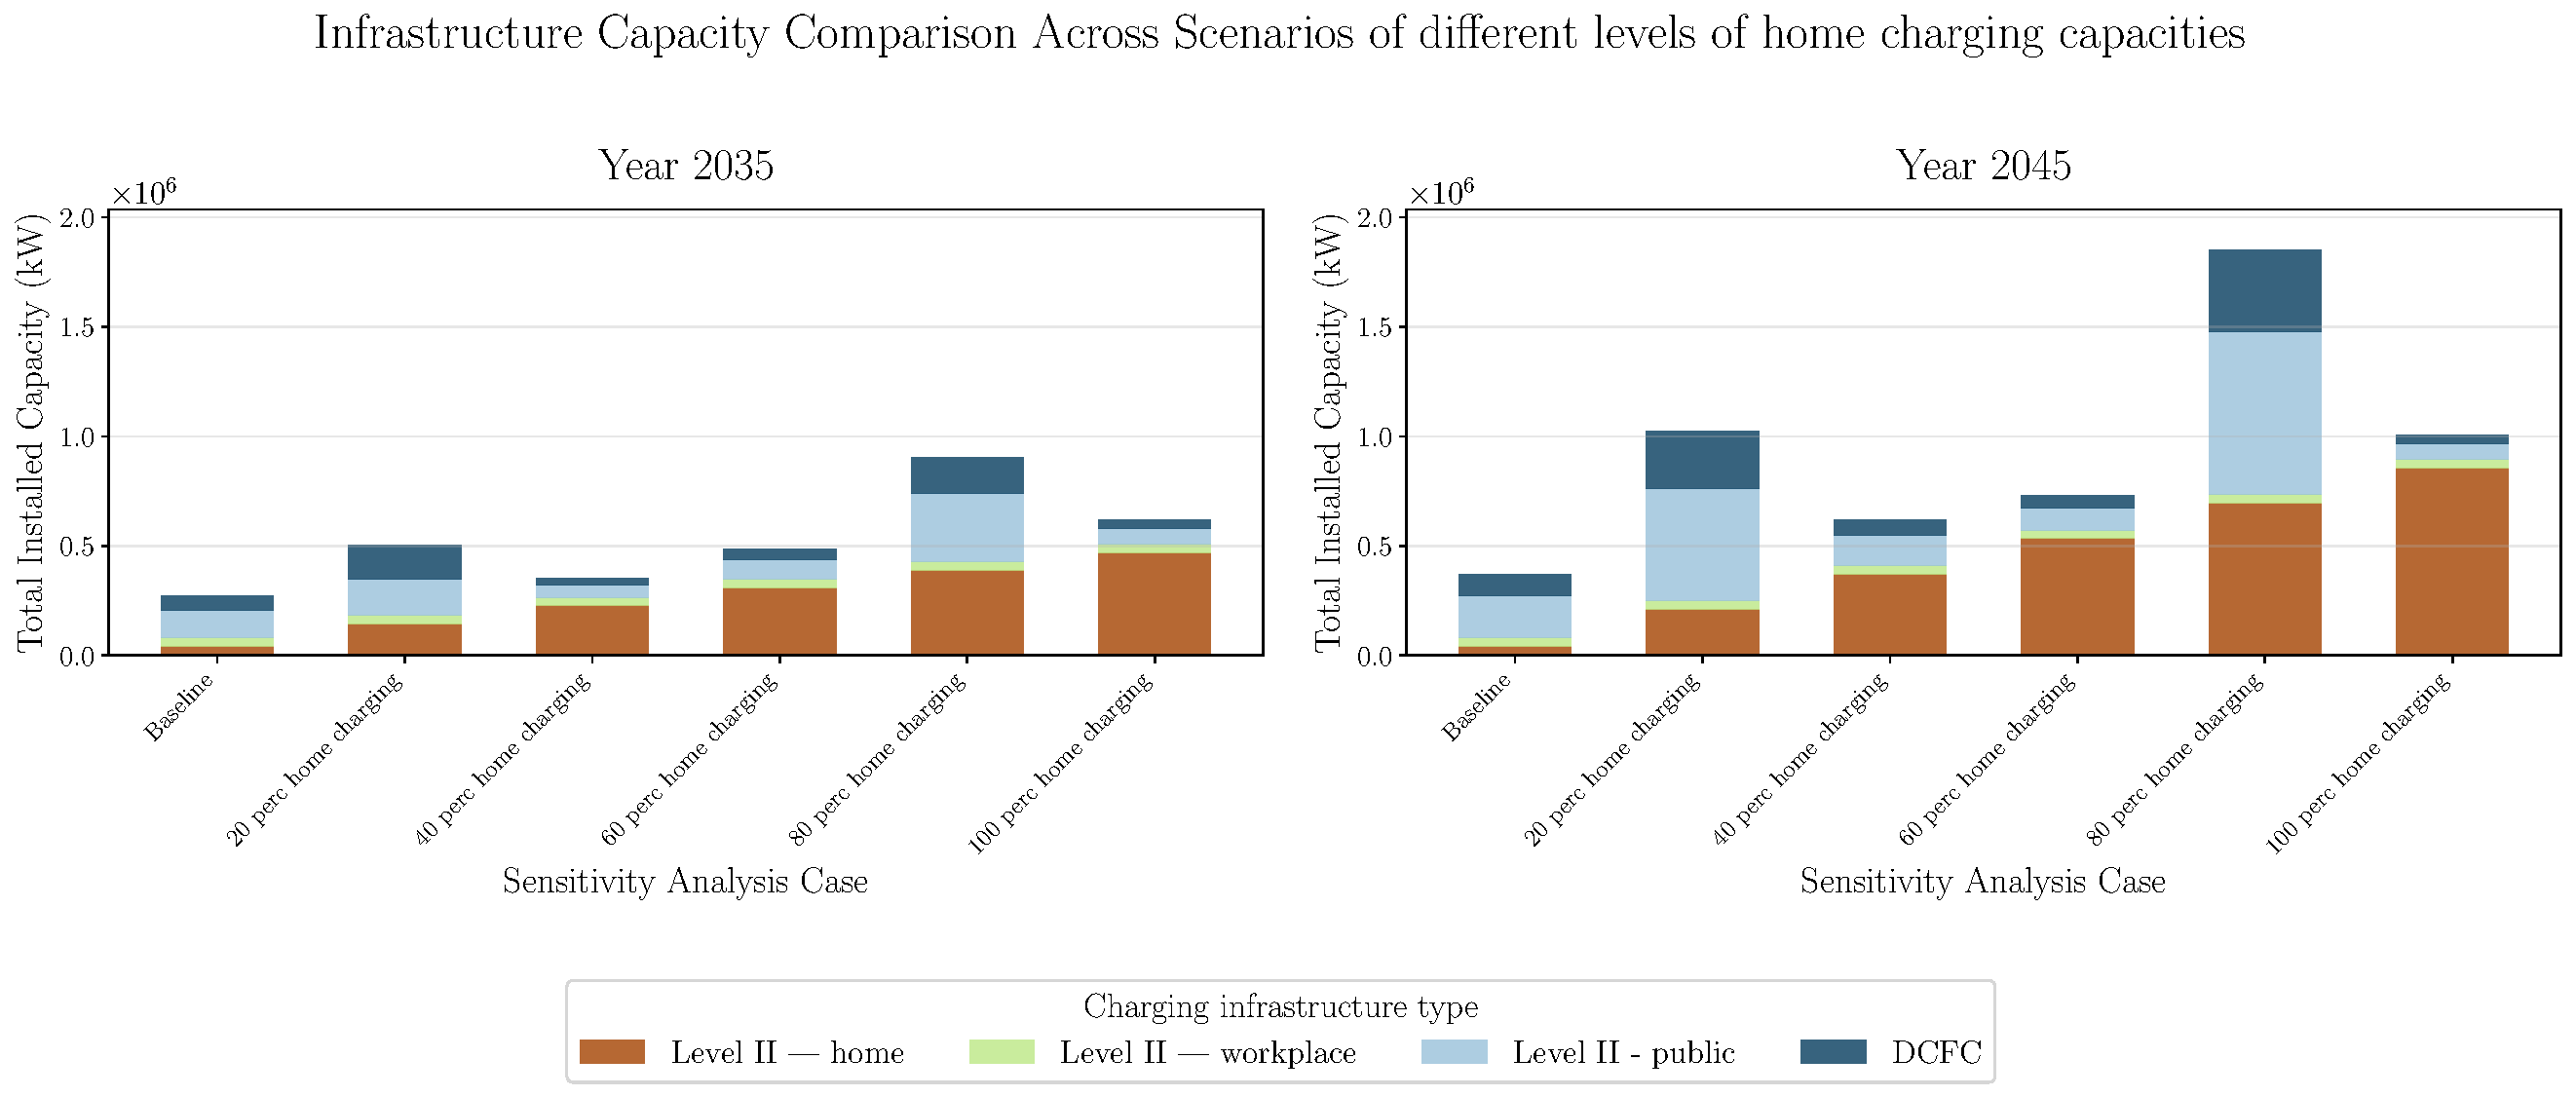
\includegraphics[width=0.9\textwidth]{graphics/SA_comparison_infrastructure_specific_years.pdf} 
%     \caption{\added{Charging infrastructure capacities by charger type installed by years 2035 and 2045 for different scenarios of home charging.}} \label{fig: SA_comp_final}
% \end{figure} 
\added{\subsection{Home charger capacities}} \label{sec:app_home}
\added{In the results presented in Section \ref{sec:res}, home charging capacities are not expanded beyond initial availability. In the following sensitivity analysis, we impose exogenously defined home charging capacities to observe the adoption of battery-electric passenger cars and charging patterns by income class under different home charging scenarios.}

\added{We model expansion scenarios for home charging capacities based on home ownership rates and maximum possible installations for home chargers, determining maximum total capacities for each income class. From these, we derive linear expansion pathways.}

\added{Figure \ref{fig: home_charging_exp_scenarios} displays the assumed home charging capacity expansions. The percentage values (20–100) represent the share of maximum home charging capacity to be reached by 2050, with linear expansion pathways. The sensitivity analysis uses the densification scenario $n^{\mathrm{points~per~site}} = 10$ as the baseline.}

\begin{figure}[H]
\centering
    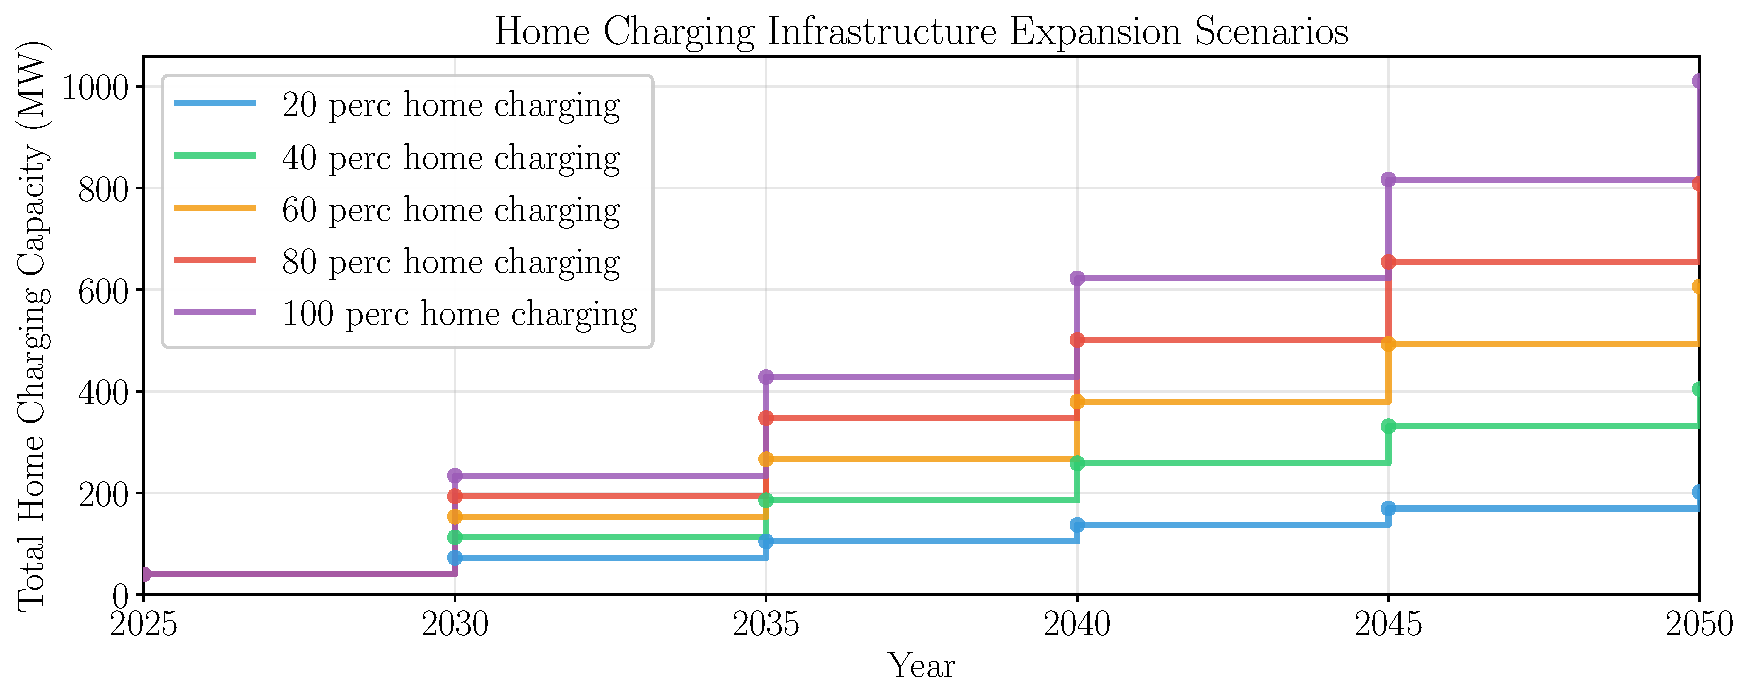
\includegraphics[width=\textwidth]{graphics/home_charging_expansion_scenarios.pdf} 
    \caption{\added{Exogenous home charging capacity expansion scenarios.}} \label{fig: home_charging_exp_scenarios}
\end{figure} 

\added{Figure \ref{fig: SA_comp_cons} displays the impact of increased home charging capacity on public charging infrastructure utilization. Higher home charging capacity shifts utilization toward home charging, reducing the role of public charging in demand coverage. However, no clear pattern is visible in fast charger utilization. Figure \ref{fig: SA_comp_final} shows capacity installations by charger type for 2035 and 2045. The increasing home charging capacity is clearly visible. In scenarios with low fast charger utilization (\textit{20 perc home charging} and \textit{80 perc home charging}), public charger capacities expand further.}

\added{The inconsistent pattern in fast charging utilization likely reflects near-indifference in the objective function between solutions with and without fast charging.}

\begin{figure}[H]
\centering
    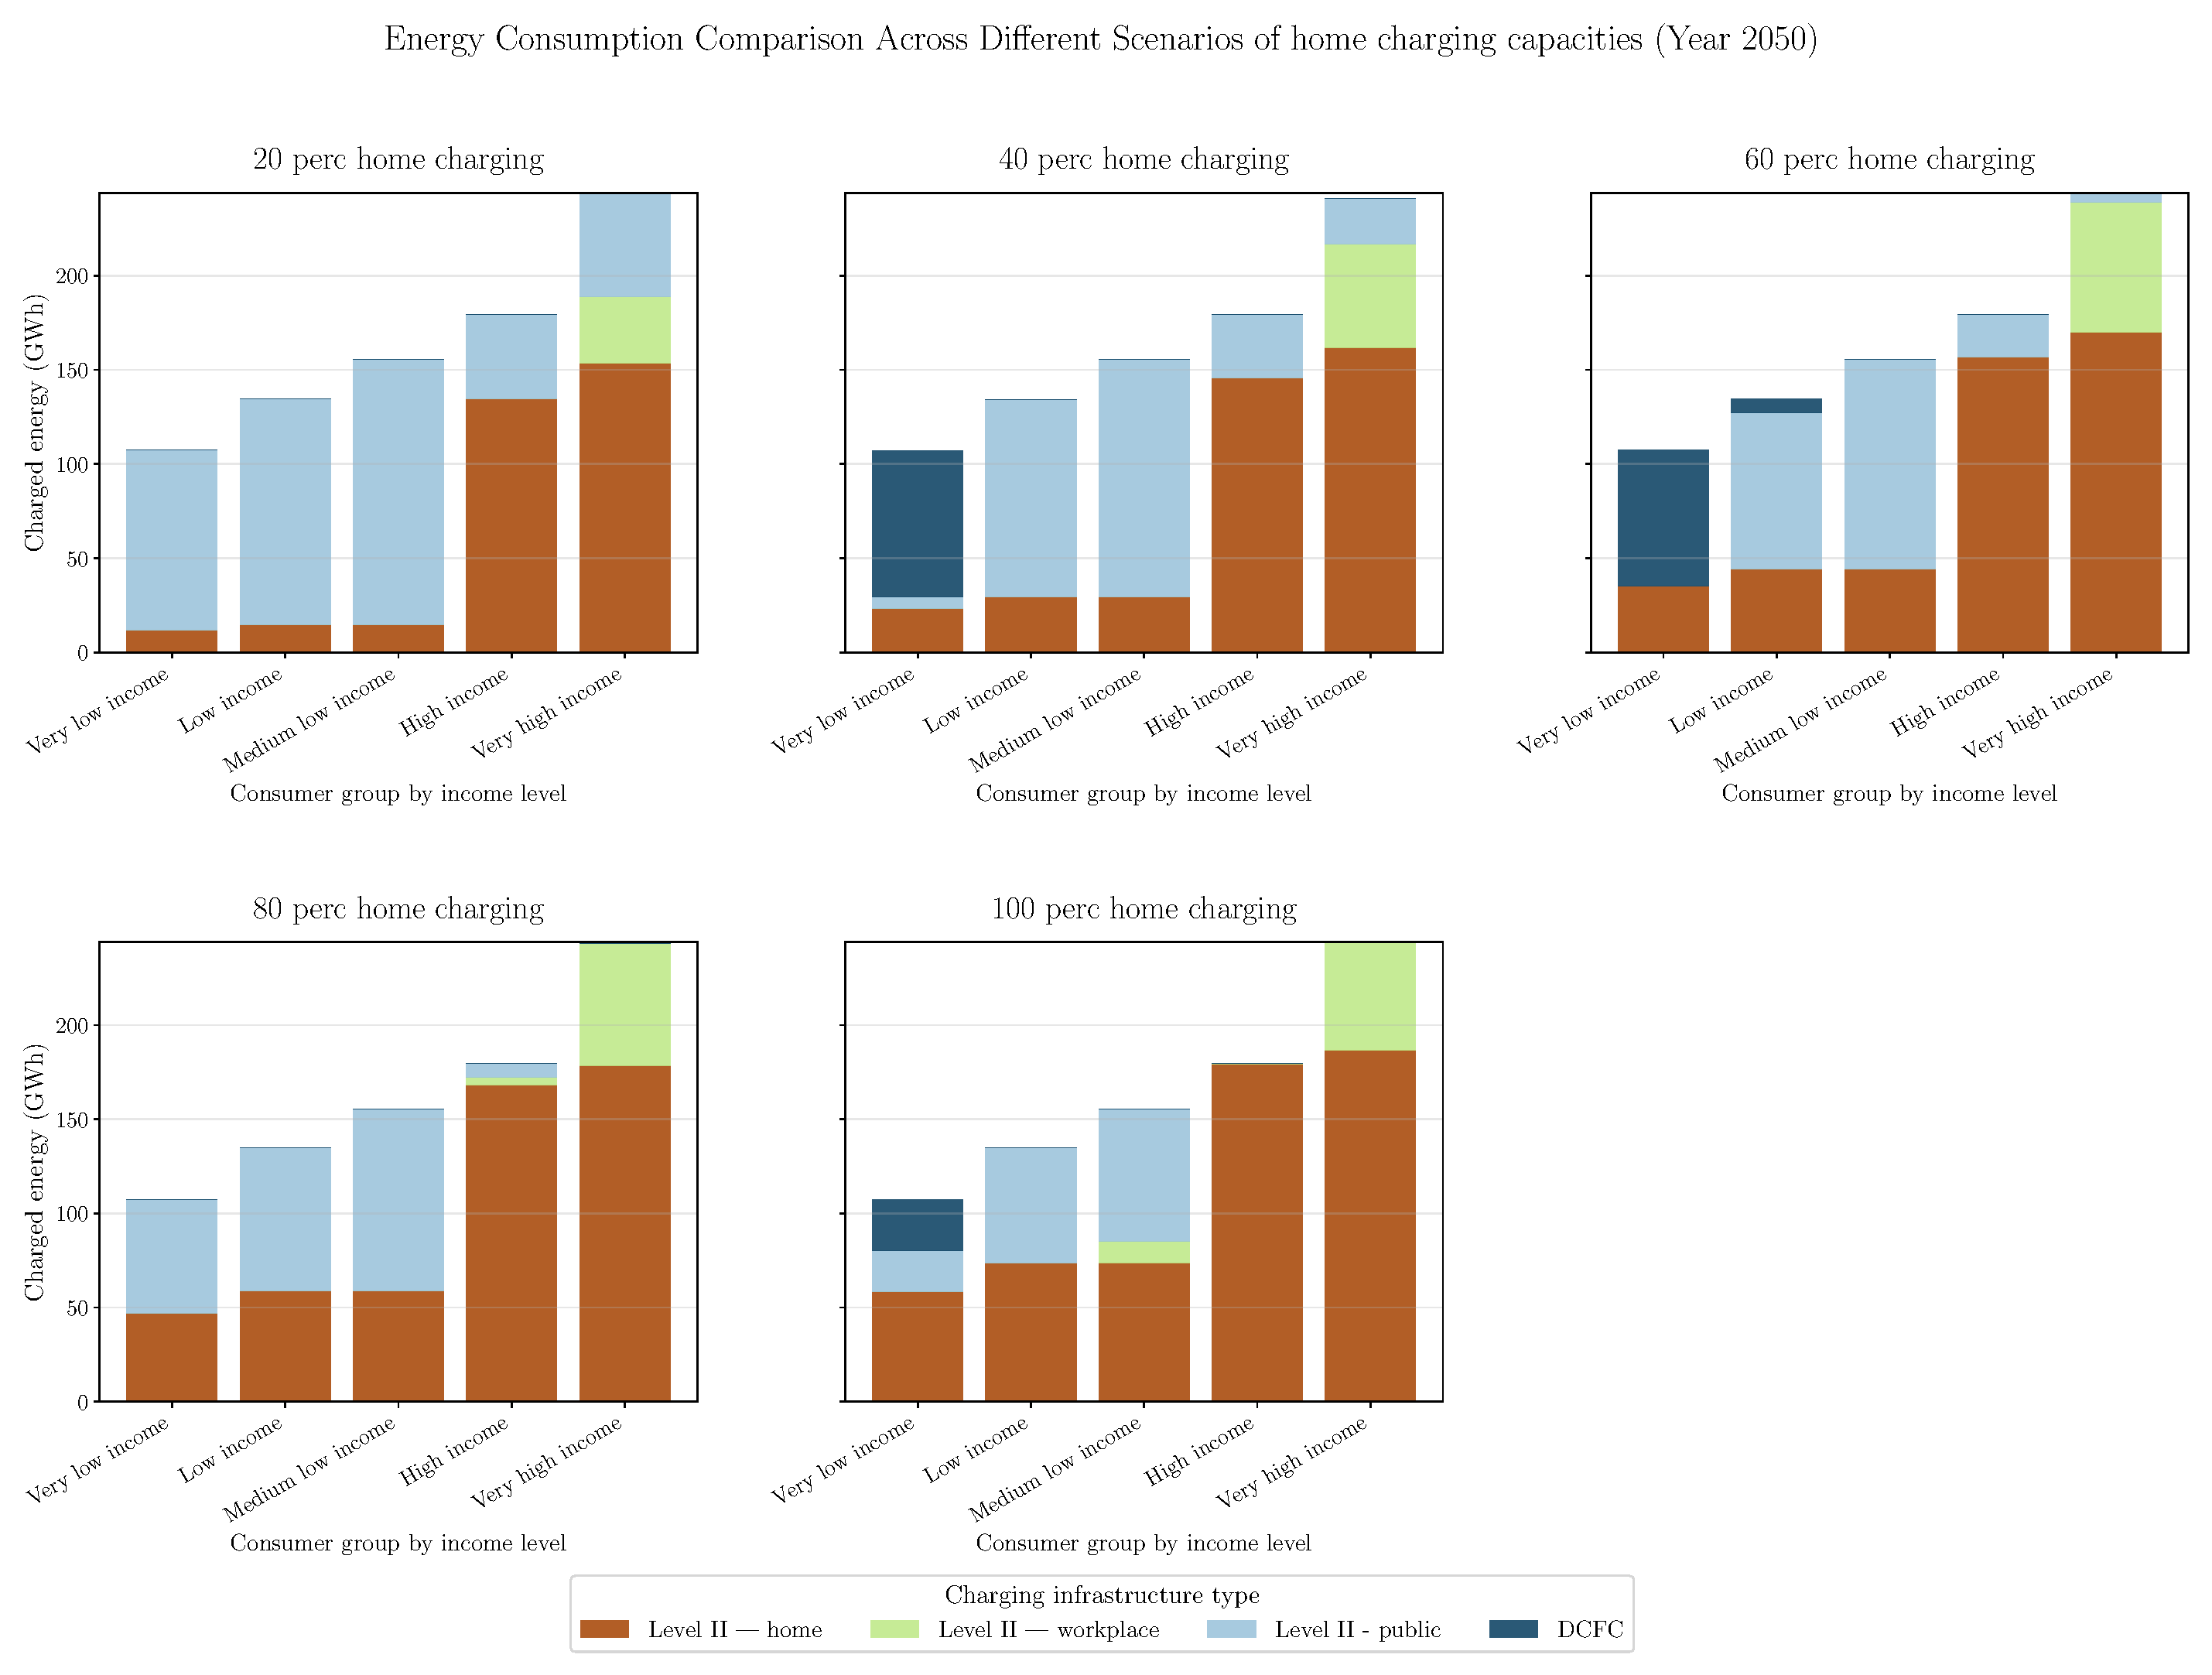
\includegraphics[width=\textwidth]{graphics/SA_comparison_energy_consumption.pdf} 
    \caption{\added{Energy consumption patterns across income classes for different exogenous home charging capacity scenarios.}} \label{fig: SA_comp_cons}
\end{figure} 

\begin{figure}[H]
\centering
    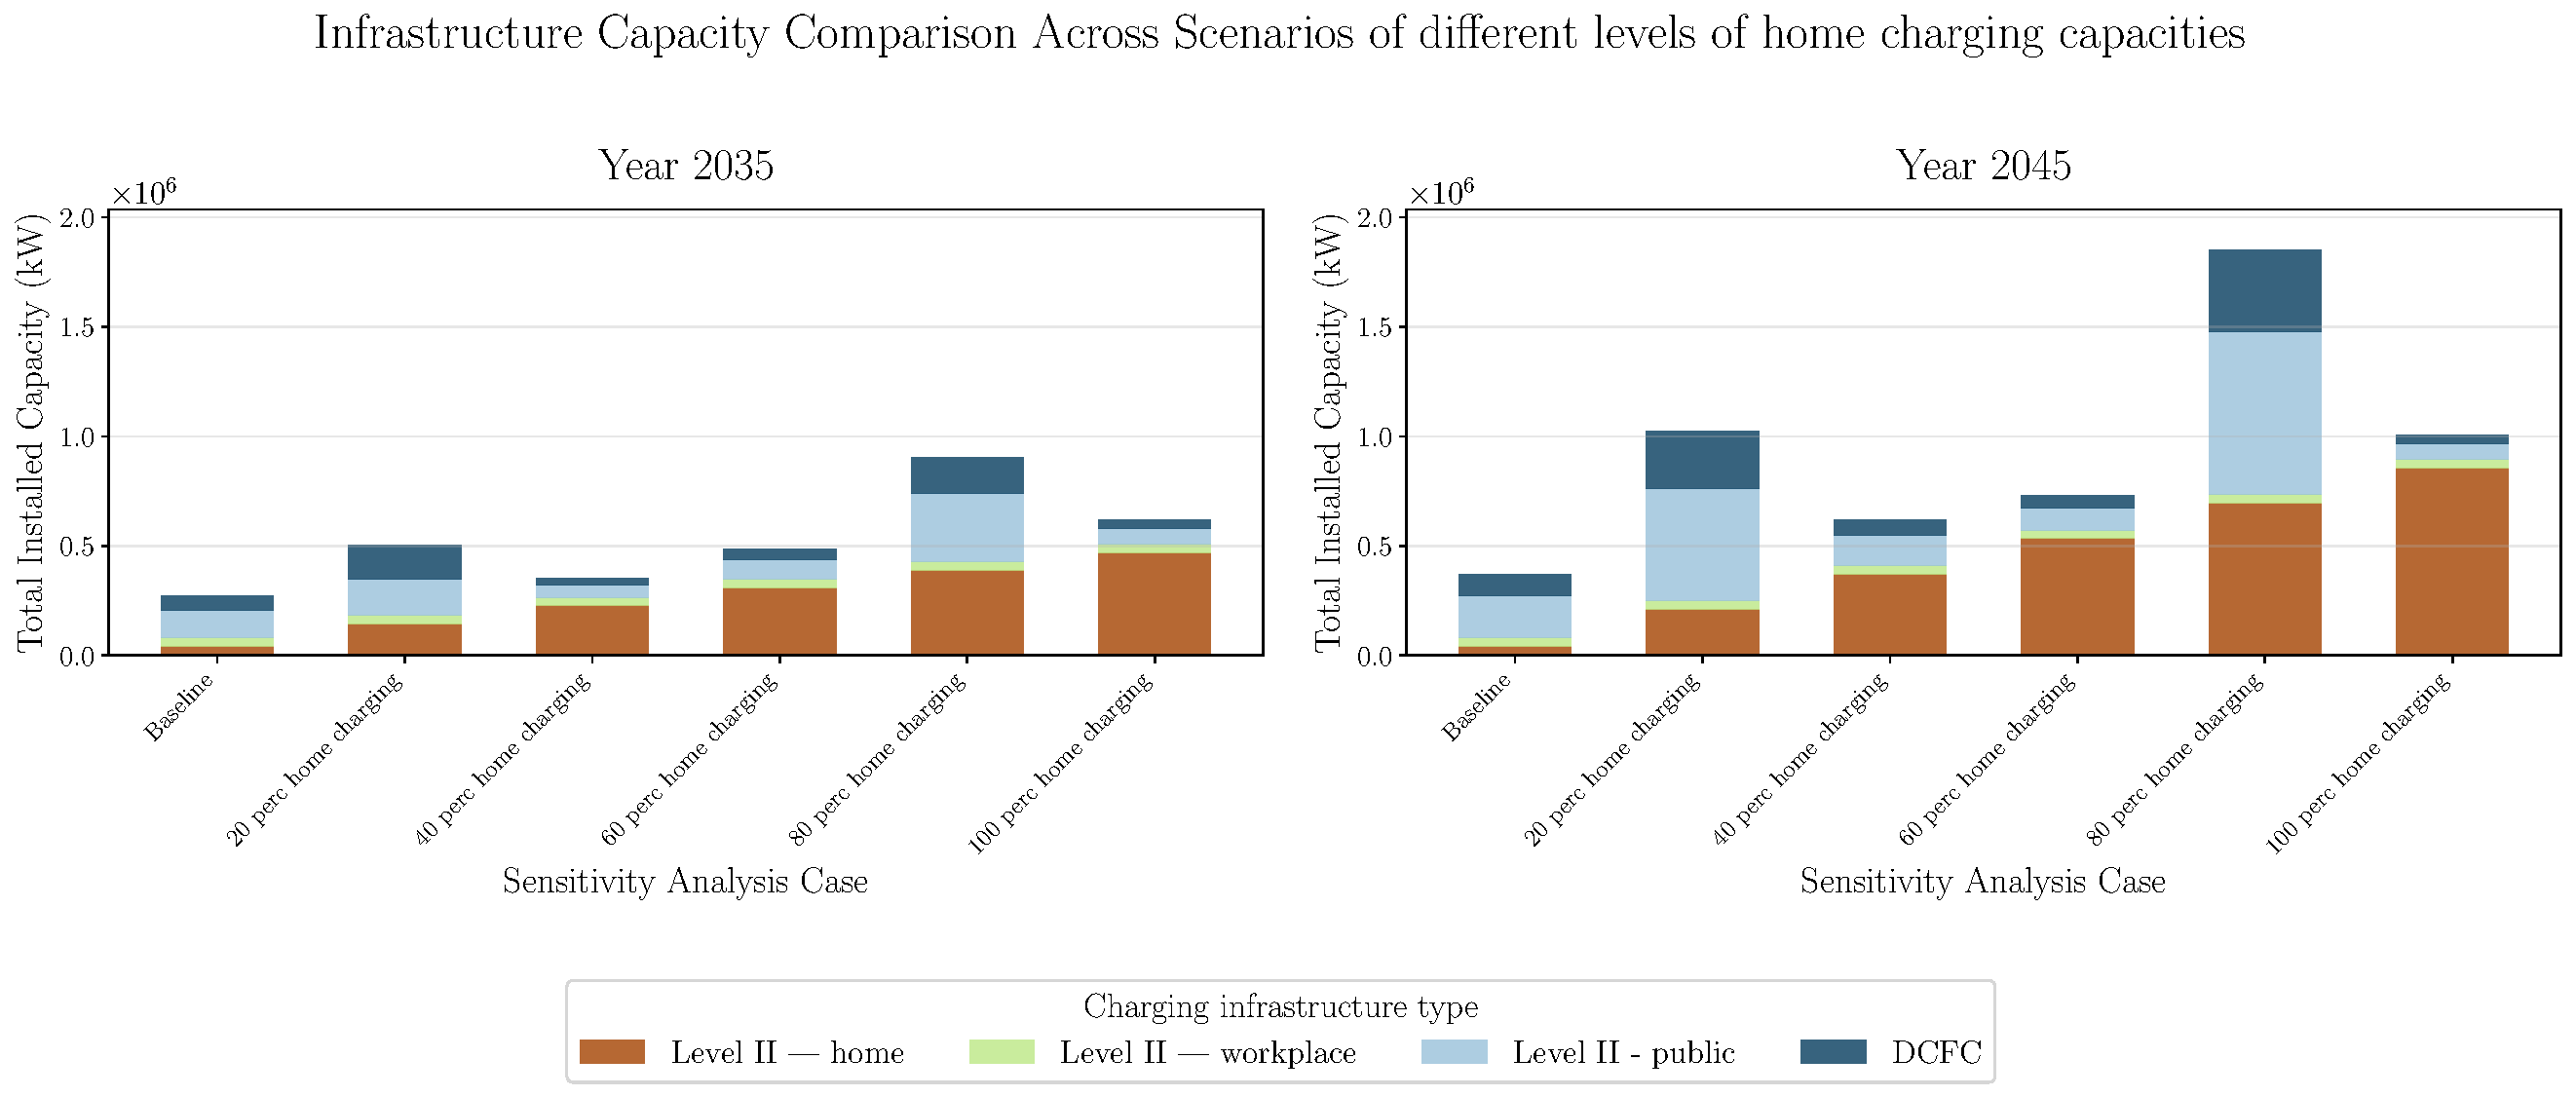
\includegraphics[width=\textwidth]{graphics/SA_comparison_infrastructure_specific_years.pdf} 
    \caption{\added{Charging infrastructure capacities by charger type for 2035 and 2045 across home charging scenarios.}} \label{fig: SA_comp_final}
\end{figure}

% \added{\subsection{Central accelerated roll-out}}

% \added{In the scenario design addressing \textit{RQ1} (described in Section \ref{sec:rq2_scendesign}), we test increased charging infrastructure in the \say{central} region Bizkaia to observe the impacct on Gipuzkoa and Araba. The public charging capacity is increased by $+30\%$. To gain better insights into other levels of increase of the charging infrastructure. }

% \added{We model two additional expansion scenarios: One with +15\% of centrally accelerated capacity expansion and one with +45\% expansion to observe how the spillover magnitude scales. Figure \ref{fig: comp_maximum_diff} displays the results indicating the peak of absolute maximum differences between the scenarios \textit{Baseline Roll-out} and \textit{Central Acc. Roll-out}. The increase impact of increased charging capacity in Bizkaia has a increasingly higher impact on the BEV adotion in Gipuzkoa than Araba. Overall, there is an increasing spillover effect with larger charging capacities in Bizkaia in similar modest extend as the results of the manuscript demonstrate.
% }
        
% \begin{figure}[H]
% \centering
%     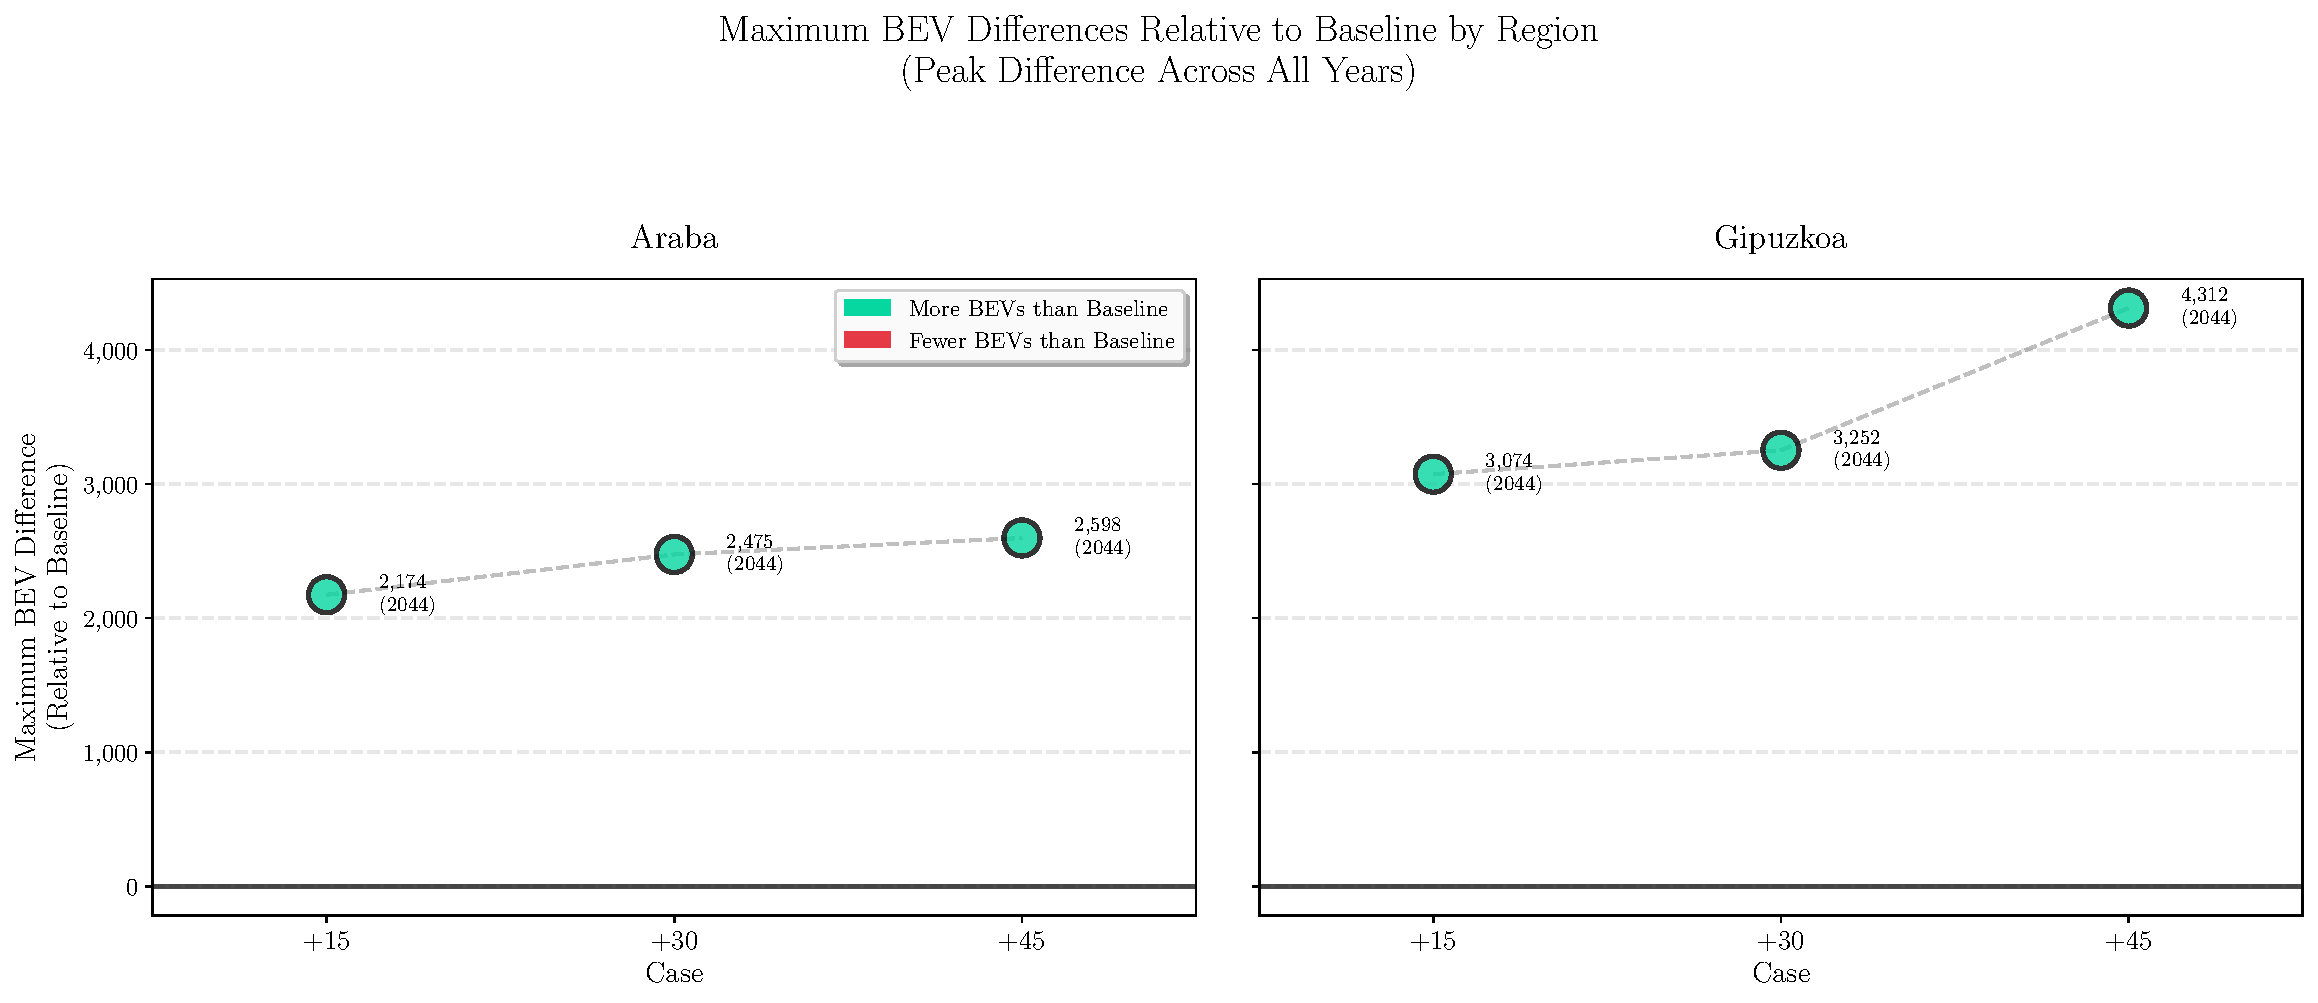
\includegraphics[width=\textwidth]{graphics/h_comparison_maximum_bev_differences_by_region.pdf} 
%     \caption{\added{Charging infrastructure capacities by charger type installed by years 2035 and 2045 for different scenarios of home charging.}} \label{fig: comp_maximum_diff}
% \end{figure} 
\added{\subsection{Central accelerated roll-out}} \label{sec:app_spillover}
\added{In the scenario design addressing \textit{RQ2} (described in Section \ref{sec:rq2_scendesign}), we test increased charging infrastructure in the central region Bizkaia to observe the impact on Gipuzkoa and Araba. In the main analysis, public charging capacity is increased by +30\%. To gain better insights into other levels of capacity increase, we model two additional expansion scenarios: +15\% and +45\% centrally accelerated capacity expansion.}

\added{Figure \ref{fig: comp_maximum_diff} displays the peak absolute differences in BEV adoption between the \textit{Baseline Roll-out} and \textit{Central Acc. Roll-out} scenarios. The impact of increased charging capacity in Bizkaia on BEV adoption is higher in Gipuzkoa than in Araba. Overall, the spillover effect increases with larger charging capacities in Bizkaia, though the magnitude remains modest, consistent with the main results.}

\begin{figure}[H]
\centering
    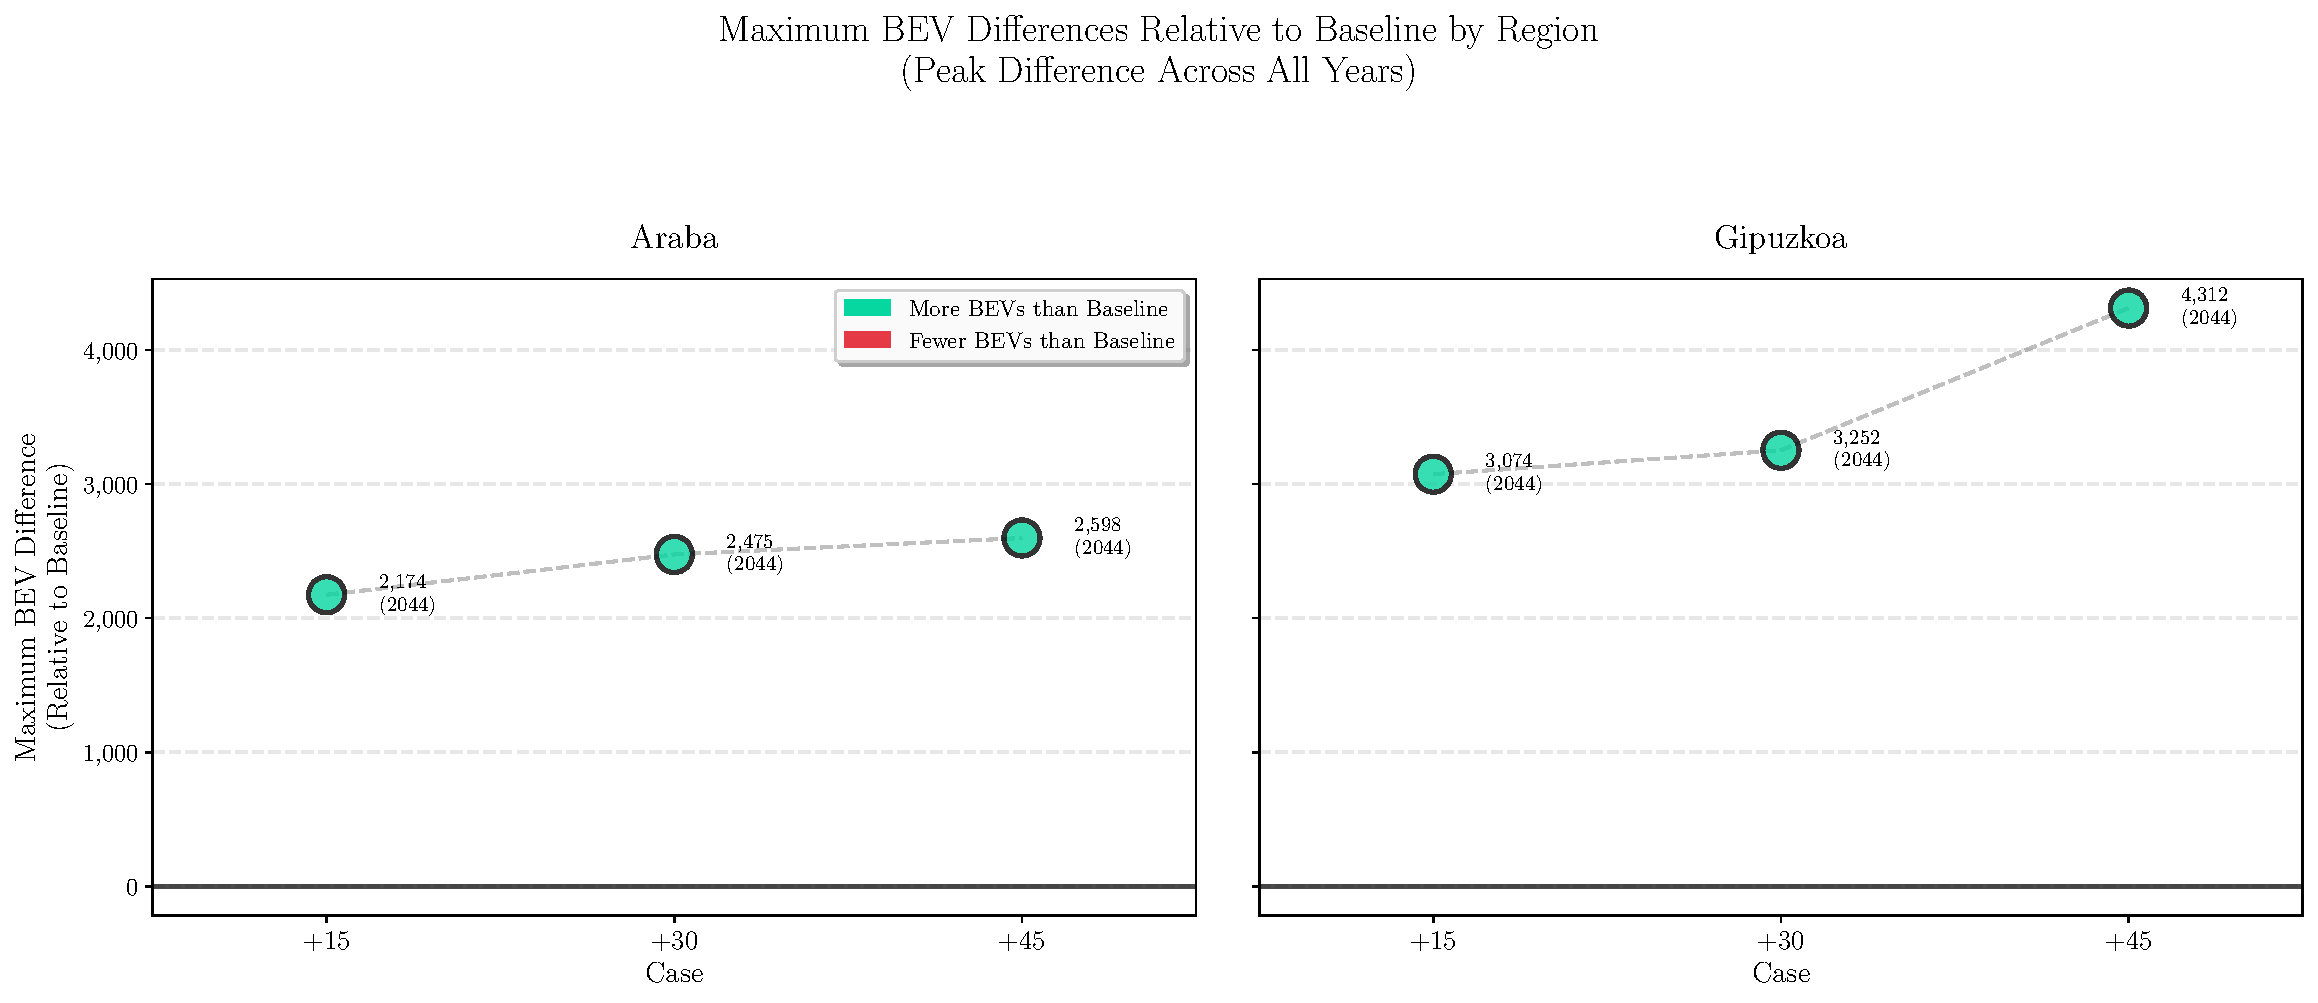
\includegraphics[width=\textwidth]{graphics/h_comparison_maximum_bev_differences_by_region.pdf} 
    \caption{\added{Peak absolute differences in BEV adoption between \textit{Baseline Roll-out} and \textit{Central Acc. Roll-out} scenarios across capacity expansion levels (+15\%, +30\%, +45\%).}} \label{fig: comp_maximum_diff}
\end{figure}





\end{document}

%%
%% End of file `elsarticle-template-num.tex'.
